% Copyright (C) 2014-2017 by Thomas Auzinger <thomas@auzinger.name>

\documentclass[draft,final]{vutinfth} % Remove option 'final' to obtain debug information.

% Load packages to allow in- and output of non-ASCII characters.
\usepackage{lmodern}        % Use an extension of the original Computer Modern font to minimize the use of bitmapped letters.
\usepackage[T1]{fontenc}    % Determines font encoding of the output. Font packages have to be included before this line.
\usepackage[utf8]{inputenc} % Determines encoding of the input. All input files have to use UTF8 encoding.

% Extended LaTeX functionality is enables by including packages with \usepackage{...}.
\usepackage{amsmath}    % Extended typesetting of mathematical expression.
\usepackage{amssymb}    % Provides a multitude of mathematical symbols.
\usepackage{mathtools}  % Further extensions of mathematical typesetting.
\usepackage{microtype}  % Small-scale typographic enhancements.
\usepackage[inline]{enumitem} % User control over the layout of lists (itemize, enumerate, description).
\usepackage{multirow}   % Allows table elements to span several rows.
\usepackage{booktabs}   % Improves the typesettings of tables.
\usepackage{subcaption} % Allows the use of subfigures and enables their referencing.
\usepackage[ruled,linesnumbered,algochapter]{algorithm2e} % Enables the writing of pseudo code.
\usepackage[usenames,dvipsnames,table]{xcolor} % Allows the definition and use of colors. This package has to be included before tikz.
\usepackage{nag}       % Issues warnings when best practices in writing LaTeX documents are violated.
\usepackage{todonotes} % Provides tooltip-like todo notes.
\usepackage{hyperref}  % Enables cross linking in the electronic document version. This package has to be included second to last.
\usepackage[acronym,toc]{glossaries} % Enables the generation of glossaries and lists fo acronyms. This package has to be included last.
\usepackage{appendix}
\usepackage{rotating}
\usepackage{float}
\usepackage{afterpage}
% Define convenience functions to use the author name and the thesis title in the PDF document properties.
\newcommand{\authorname}{Rebeka Koszticsak} % The author name without titles.
\newcommand{\thesistitle}{Enhancement of Footwear Impressions} % The title of the thesis. The English version should be used, if it exists.

% Set PDF document properties
\hypersetup{
    pdfpagelayout   = TwoPageRight,           % How the document is shown in PDF viewers (optional).
    linkbordercolor = {Melon},                % The color of the borders of boxes around crosslinks (optional).
    pdfauthor       = {\authorname},          % The author's name in the document properties (optional).
    pdftitle        = {\thesistitle},         % The document's title in the document properties (optional).
    pdfsubject      = {Subject},              % The document's subject in the document properties (optional).
    pdfkeywords     = {a, list, of, keywords} % The document's keywords in the document properties (optional).
}

\setpnumwidth{2.5em}        % Avoid overfull hboxes in the table of contents (see memoir manual).
\setsecnumdepth{subsection} % Enumerate subsections.

\nonzeroparskip             % Create space between paragraphs (optional).
\setlength{\parindent}{0pt} % Remove paragraph identation (optional).

\makeindex      % Use an optional index.
\makeglossaries % Use an optional glossary.
%\glstocfalse   % Remove the glossaries from the table of contents.

% Set persons with 4 arguments:
%  {title before name}{name}{title after name}{gender}
%  where both titles are optional (i.e. can be given as empty brackets {}).
\setauthor{}{\authorname}{Bsc}{male}
\setadvisor{Ao.Univ.Prof. Dipl.-Ing. Dr.techn.}{Robert  Sablatnig}{}{male}

% For bachelor and master theses:
\setfirstassistant{Associate Prof.}{Hideki Nakayama}{Ph.D.}{male}
\setsecondassistant{Projektass. Dipl.-Ing.}{Manuel  Keglevic}{}{male}
%\setthirdassistant{Pretitle}{Forename Surname}{Posttitle}{male}

% For dissertations:
%\setfirstreviewer{Pretitle}{Forename Surname}{Posttitle}{male}
%\setsecondreviewer{Pretitle}{Forename Surname}{Posttitle}{male}

% For dissertations at the PhD School and optionally for dissertations:
%\setsecondadvisor{Pretitle}{Forename Surname}{Posttitle}{male} % Comment to remove.

% Required data.
\setaddress{Address}
\setregnumber{01325492}
\setdate{04}{01}{2020} % Set date with 3 arguments: {day}{month}{year}.
\settitle{\thesistitle}{Enhancement of Footwear Impressions} % Sets English and German version of the title (both can be English or German). If your title contains commas, enclose it with additional curvy brackets (i.e., {{your title}}) or define it as a macro as done with \thesistitle.
%\setsubtitle{Optional Subtitle of the Thesis}{Optionaler Untertitel der Arbeit} % Sets English and German version of the subtitle (both can be English or German).

% Select the thesis type: bachelor / master / doctor / phd-school.
% Bachelor:
%\setthesis{bachelor}
%
% Master:
\setthesis{master}
\setmasterdegree{dipl.} % dipl. / rer.nat. / rer.soc.oec. / master
%
% Doctor:
%\setthesis{doctor}
%\setdoctordegree{rer.soc.oec.}% rer.nat. / techn. / rer.soc.oec.
%
% Doctor at the PhD School
%\setthesis{phd-school} % Deactivate non-English title pages (see below)

% For bachelor and master:
\setcurriculum{Visual Computing}{Visual Computing} % Sets the English and German name of the curriculum.

% For dissertations at the PhD School:
%\setfirstreviewerdata{Affiliation, Country}
%\setsecondreviewerdata{Affiliation, Country}


\begin{document}

\frontmatter % Switches to roman numbering.
% The structure of the thesis has to conform to
%  http://www.informatik.tuwien.ac.at/dekanat

\addtitlepage{naustrian} % German title page (not for dissertations at the PhD School).
\addtitlepage{english} % English title page.
\addstatementpage

\begin{danksagung*}
\todo{Ihr Text hier.}
\end{danksagung*}

\begin{acknowledgements*}
\todo{Enter your text here.}
\end{acknowledgements*}

\begin{kurzfassung}
\todo{Ihr Text hier.}
\end{kurzfassung}

\begin{abstract}
\par
Shoeprint images are evidences secured on crime scenes.
Even though automatic shoeprint processing is a highly researched topic, the final identification is usually done by human forensic experts.
\par
This thesis investigates the possibilities for enhancement of shoeprint samples from a real-life dataset, for which three prototypical approaches are presented and evaluated.
The main challenge of this task is to correctly filter the pattern of the shoeprint regardless of the versatile, possibly heavily structured and cluttered noise on the samples.
Among fully automated methods, a semi-automated technique is also tested, where user input is required for noise separation.
\par
The aim of this work is to give an overview about the current state of the art and to define an approach which is able to filter and enhance the shoeprint data despite the presence of noise and varying image quality.
Along two fully-automated algorithms a semi-automated noise-suppression and enhancement pipeline for shoeprint images is introduced. 
The noisy pixels are identified based on the Fourier-Mellin features of a background pixel selected by the user.
At the same time a noise model is calculated to eliminate that structure on the shoeprint pattern as well.
Additionally, the pixels are clustered based on their gradients and the non-local means approach is applied.
The experimental results show that the processed images are clearer, the pattern is sharper, the noise is masked in the detected background area and suppressed in the foreground region.
Furthermore besides qualitative evaluation also a quantitative evaluation is performed using three basic image descriptor features and the results show that the enhanced images achieve higher accuracy than the original images.


\end{abstract}

% Select the language of the thesis, e.g., english or naustrian.
\selectlanguage{english}

% Add a table of contents (toc).
\tableofcontents % Starred version, i.e., \tableofcontents*, removes the self-entry.

% Switch to arabic numbering and start the enumeration of chapters in the table of content.
\mainmatter

\chapter{Introduction}

\par
Shoeprints found on crime scenes are important clues or evidences during criminal investigation \cite{kong2014novel}.
Even though at one third of the crime scenes usable shoe patterns are secured \cite{alexandre1996computerized}, human input is required to recognize and analyze the found patterns  \cite{wang2014automatic}.
The work of forensic experts is not only time consuming and expensive, but there is no guarantee about the objectivness of the final outcome\cite{gueham2008automatic}.
Furthermore, the stages of the human matching process are not necessarily reproducible considering the opinions of multiple experts.
\par
There is an excessive amount of research already done in order to help or replace the work of forensic experts \cite{rida2019forensic}.
However this task is challanging because of the versatility of conditions, the features and properties of the pattern on the shoe, like age, material, etc., the characteristics of the ground where the shoeprint is left and environmental conditions, for example weather, highly influence the overall appearance of the acquired sample.
Figure \ref{fig:int:varying} shows samples of the same shoe captured under different conditions from the FID-300 \cite{kortylewski2014unsupervised} dataset.
Such high amount of factors results in changing appearance causing high intra-class variance while searching for common features of the same shoeprint pattern.
To make the features more robust and to lower the influence of those factors sheprint enhancement is proposed.
\par
In 2014 a new dataset called FID-300 \cite{kortylewski2014unsupervised} was released that consists shoeprint samples collected by the police. 
It contains over 1000 reference shoeprint patterns acquired in a laboratory.
Moreover, the database introduces 300 new real-life shoeprint samples providing an insight to images forensic experts work with on a daily basis.

\begin{figure}[h]
  \centering
  \begin{subfigure}[t]{0.13\columnwidth}
    \centering
    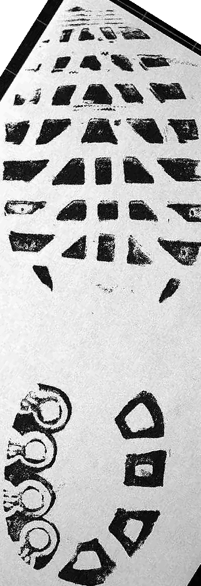
\includegraphics[width=\textwidth]{1/00003.jpg}
	\caption{}
	\label{fig:int:varying:3}
  \end{subfigure}
   \begin{subfigure}[t]{0.13\columnwidth}
    \centering
    \includegraphics[width=\textwidth]{1/00009.jpg}
	\caption{}
	\label{fig:int:varying:9}
  \end{subfigure}
 \begin{subfigure}[t]{0.13\columnwidth}
    \centering
    \includegraphics[width=\textwidth]{1/00017.jpg}
	\caption{}
	\label{fig:int:varying:17}
  \end{subfigure}
 \begin{subfigure}[t]{0.13\columnwidth}
    \centering
    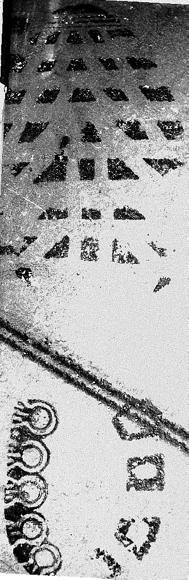
\includegraphics[width=\textwidth]{1/00020.jpg}
	\caption{}
	\label{fig:int:varying:20}
  \end{subfigure}
 \begin{subfigure}[t]{0.13\columnwidth}
    \centering
    \includegraphics[width=\textwidth]{1/00021.jpg}
	\caption{}
	\label{fig:int:varying:21}
  \end{subfigure}
 \begin{subfigure}[t]{0.13\columnwidth}
    \centering
    \includegraphics[width=\textwidth]{1/00025.jpg}
	\caption{}
	\label{fig:int:varying:25}
  \end{subfigure}
 \begin{subfigure}[t]{0.13\columnwidth}
    \centering
    \includegraphics[width=\textwidth]{1/00066.jpg}
	\caption{}
	\label{fig:int:varying:66}
  \end{subfigure}
  \caption{Example images from the FID-300 \cite{kortylewski2014unsupervised} dataset, where the soheprint is captured under different conditions.}
  \label{fig:int:varying}
\end{figure}

\section{Problem Definition}
\par
This work focuses on the ways of increasing the sample quality in terms of the amount of noise on the image and the intensity difference between the fore- and the background.
Since the already available methods are evaluated on different datasets a comparison between them is a challenging task.
Furthermore, they focus on the definition of robust descriptor and a powerful matching algorithm to overcome the problem of versatile appearance of the shoeprints.
In this thesis three prototypical preprocessing techniques are developed and tested to enhance the shoeprint samples and to make the extracted features more accurate. 
\par
For evaluation and testing the FID-300 database is used.
The dataset contains both reference prints as well as on a crime secured, real shoeprint patterns.
Additionally, the Ground Truth about every real sample and its belonging reference print is also available.
The goal of this work is to define an image processing pipeline which correctly identifies and enhances the shoe patterns and eliminates or suppresses the noise on the pattern samples regardless of the quality of the image.
A secondary objective is to gain an overview about the preformance of the algorithms, and make an estimation which methods are applicable in real-life scenarios based on their performance on the FID-300 database. 

\begin{figure}[h]
  \centering
  \begin{subfigure}[t]{0.45\columnwidth}
    \centering
    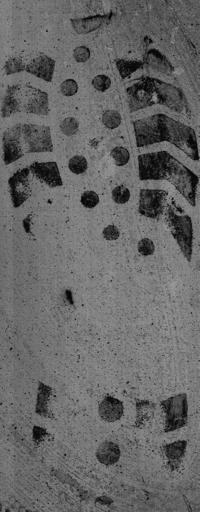
\includegraphics[width=\textwidth]{1/00219.jpg}
	\caption{}
	\label{fig:int:cap:pos}
  \end{subfigure}
  \begin{subfigure}[t]{0.45\columnwidth}
    \centering
    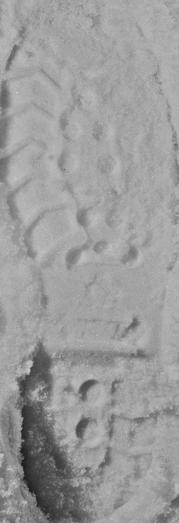
\includegraphics[width=\textwidth]{1/00217.jpg}
	\caption{}
	\label{fig:int:cap:neg}
  \end{subfigure}
  \caption{Example shoeprint impressions from FID-300 where the positive and the negative image of the same shoeprint is captured}
  \label{fig:int:cap}
\end{figure}


\afterpage{
\begin{figure}[H]
  \centering
  \begin{subfigure}[t]{0.45\columnwidth}
    \centering
    \includegraphics[width=\textwidth]{1/00182.jpg}
    \subcaption{Example image from the FID-300 database}
    \label{fig:intro:orig}
  \end{subfigure}
  \begin{subfigure}[t]{0.45\columnwidth}
    \centering
    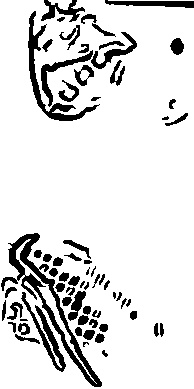
\includegraphics[width=\textwidth]{1/00182_filtered.jpg}
    \subcaption{Enhanced image}
    \label{fig:intro:enhanced}
  \end{subfigure}
  \caption{Result of the proposed algorithm. The background is correctly masked and the contrast between fore- and background is increased. On the bottom right area a weakness of the algorithms is shown, where small pattern structures were wrongly eliminated.  }
  \label{fig:example}
\end{figure}
}

\section{Challenges}
\par
An obstacles in the topic of shoeprint enhancement and in automatic shoeprint matching in general is the versatile image quality and appearance.
There are approaches available which build models for given structures of the shoeprint \cite{tang2010footwear}, \cite{alizadeh2017automatic}, but they are limited to given parts of the shoesole and are tested on a restricted database.
Moreover, there is an inference from noise of multiple sources.
Firstly, the produced shoeprint and its background depends on the properties of the ground where the impression was made, the roughness and unevenness of a given type of surface distorts the original shoe sole pattern and those features on the ground appear as noise on the final sample.
The impressions of Figure \ref{fig:int:varying:3} and \ref{fig:int:varying:20} were made on an even surface whereas on Figure \ref{fig:int:varying:17} and \ref{fig:int:varying:25} cluttered background is visible caused by the surface properties.
Furthermore, objects on the surface, above or behind the left shoeprint potentially cover or distort the original pattern, or prevent to secure the complete area of the original shoe sole.
On Figures \ref{fig:int:varying:9} and \ref{fig:int:varying:66} only partial shoeprints were secured, on the left side of Figure \ref{fig:int:varying:66} the structures of the shoe sole pattern are hardly visible because of the additional noise.
Other than that illumination changes occur as well \ref{fig:int:varying:20}.
Besides, the pattern on the original shoe can also be distorted or modified.
These alterations possibly contain valuable information about the owner, however, they make it more difficult to match the pattern with the reference prints captured on unused shoes.
Additionally, there are multiple shoeprint securing methods producing different results for the same print \cite{katireddy2017novel}. 
The shoeprint securing technique used depends on the properties of the ground. 
The securing method and the additional properties of the floor, for example if it was clean or dusty when making an impression, also determine if the positive \ref{fig:int:cap:pos} or the negative \ref{fig:int:cap:neg}, the pattern or the space between them, image is captured.
Furthermore, the majority of the publications focus on the development of robust feature sets and matching algorithms and not on the preprocessing of the shoeprint samples, therefore there  is limited knowledge available about the specific domain of shoeprint enhnacement.
Proposed methods for forensic shoeprint matching are discussed in the following chapter.

\par
As mentioned previously the already published methods were tested and evaluated on different datasets, thus a comparison between them is difficult.
Moreover, the used dataset is not necessarily public \cite{katireddy2017novel}, \cite{dardi2009texture} making it impossible to reproduce the result in such cases.
Additionally, the handcrafted databases can be biased, and allow such restrictions and modifications that do not correlate with real-life scenarios \cite{rida2019forensic}.
The used samples are either synthetically generated, they are secured in a laboratory for the purpose of evaluating forensic image processing algorithms, and computationally distorted \cite{de2005automated}, \cite{gueham2008automatic} or exclude images by a given criteria, for example quality and noise \cite{dardi2009texture}, \cite{tang2010footwear}.
The time consuming approach of re-implementation of the available algorithms and testing them on the FID-300 is also impossible in the cases, where the original dataset of the publication is not accessible.
Thus it is challenging to plan a new algorithm based on the published results because the lack of a uniform baseline.

\section{Contribution}
\par
In this thesis an overview about shoeprint enhancement methods is given.
Multiple approaches are implemented, discussed and evaluated.
Two ways to increase the quality, defined as the contrast between the fore- and the background, of a given shoeprint sample are to enhance the pattern regardless of the noise and to suppress or eliminate the noise without losing any pattern information.
Along fully-automated methods semi-automated algorithms are also considered.
Three different approaches are introduced and examined in respect to their performance on real-life image samples.
\par
Finally, a semi-automated framework is presented which is evaluated on the FID-300 database.
In the first step user input specifying the noise is required.
The input is separated into tiles, and the subparts are compared based on the Fourier-Mellin features of the given region and of the neighborhood selected by the user.
In that way the background is separated from the foreground and a noise model based on the background is determined.
Since noise appears on the pattern as well, those parts are corrected according to the calculated noise model.
After that, the pixels are classified based on their gradients and the non-local means algorithm is applied.
According to the amount of members of each class shoeprint and noise classes are determined.
Finally, candidates of the latter are eliminated.
The final image is thresholded to create a binary image, where the shoeprint is recognizable because the clutter is suppressed on the pattern and masked on the background.
Throughout the whole processing pipeline morphological operations and small structure elimination are applied multiple times. 
First when a mask for background is built, and also in the end of the pipeline to eliminate small inconsistencies on the determined foreground and detected lines. 
The noise elimination is based on two assumptions.
First the area selected by the user is representative for the entire image and there is a high contrast between background and shoeprint areas.
Second, the edges of the shoeprint impression share similar properties, such as gradient information, frequency as well as overall area and length, and are different from those deriving from cluster of the image.
Figure \ref{fig:example} shows an example from the FID-300 database \ref{fig:intro:orig} and the enhanced image \ref{fig:intro:enhanced} using the above algorithm.
The background of the algorithm is masked successfully and the contrast between the shoeprint impression and the background is increased.
However, in the bottom right corner of the image the weakness of the enhancement method is also shown.
Small line structures of the original shoe sole pattern resemble the short and fine edges of the noise on the sample and are wrongly eliminated.
The detailed evaluation of the proposed algorithm is presented in Chapter 4.
Experimental results show that the enhanced images are clearer, the background is successfully separated and the shoeprint pattern is less noisy than on the original images.
Moreover, the improved images have a better matching rate than their original version according to the experiments conducted on the enhanced images, on the original samples and on the reference images using three common image features such as Fourier-Mellin, SIFT and SURF.

\section{Structure of the Work}
\par
To gain an overview about the research already done the following section, Chapter 2, gives a review of the literature. 
Along papers published on the topic of shoeprint identification, matching and enhancement, research on similar domains is presented as well.
Consequently, fields of fingerprint processing and tattoo identification is also overviewed for possibilities of utilizing their solutions in the given problem space.
Furthermore, natural image enhancement and denoising techniques are revised as well.
\par
In Chapter 3 the approaches for enhancement are given.
The first section presents and reviews an algorithm for detecting shoe pattern on varying conditions.
The second one describes an automated noise suppression pipeline.
In the last section an algorithm for enhancing real-life crime scene shoeprint impressions from FID-300 is proposed.
Details on implementation are given as well.
\par
In Chapter 4 experimental results are shown and the proposed algorithms are evaluated whether they are applicable for real-life forensic images.
In Chapters 5 prospective future work is discussed and the final conclusion is given. 

\chapter{Related Work}
\par
In order to find and develop an effective algorithm for shoeprint enhancement, an overview about relevant research is made first.
Along the literature of image enhancement and noise removal, a related topic, discriminative image descriptors, is also considered to gain better insight and to define an approach which is optimized for the rest of the shoeprint identification pipeline.
In this chapter the research on the domain of shoeprint identification is reviewed.
Other than that publications from similar domains such as fingerprint and palmprint detection as well as tattoo identification are described.
Research for fingerprint identification and tattoo recognition have been chosen for review because of their similar goal of edge structure and minimal image structure recognition.
Moreover, an overview of techniques from the field of natural image enhancement and description along with general image denoising is also given.
This chapter is separated into three parts, first, Image Enhancement techniques are described, after that algorithms developed for Noise Removal specifically are discussed, and lastly, proposed Image Descriptors are reviewed.


\section{Image Enhancement}
\label{sec:rw:ImageENhancement}

In this section image enhancement techniques from four specific domains are discussed, these are shoe- and fingerprint identification, tattoo recognition and natural image enhancement.

\section*{Shoeprint Enhancement}

\par
There is an extensive research done in the field of enhancing shoeprint images \cite{rida2019forensic}.
However,  the problem definition and the use-case of the different publications varies strongly.
Because of the absence of a common database, the discussed algorithms are separated into two groups, techniques tested on synthetic samples, on shoeprint impressions generated for the purpose of evaluation of shoeprint identification algorithms, and on real-life impressions.
In a synthetic dataset the noise derives from scanning artifacts and computationally added distortions and modification.
Furthermore, a group of algorithms developed for real crime-scene data makes restrictions about the input image and exclude images by a predefined criteria, for example noise and quality.
Figure \ref{fig:rw:database} shows example images from a synthetic \ref{fig:rw:synthetic}, from a restricted \ref{fig:rw:restricted} and high \ref{fig:rw:highFID} and low quality samples \ref{fig:rw:lowFID} from the FID-300 dataset.
In the following discussion it is noticed repeatedly, which kind of dataset the proposed approach was tested on.

\begin{figure}[h]
  \centering
  \begin{subfigure}[t]{0.24\columnwidth}
    \centering
    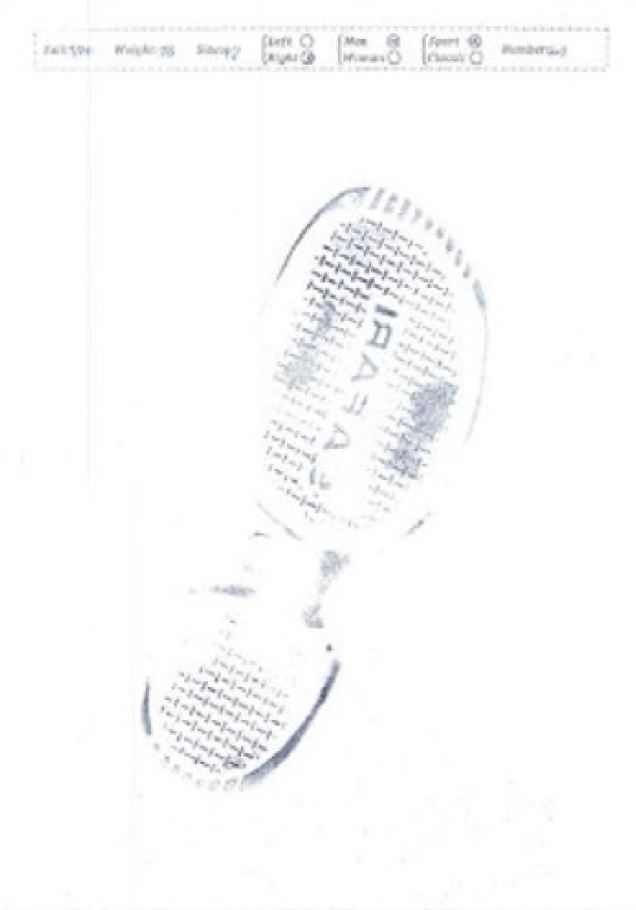
\includegraphics[width=\textwidth]{2/synthetic.jpg}
    \subcaption{Example image from a synthetic dataset}
    \label{fig:rw:synthetic}
  \end{subfigure}
  \begin{subfigure}[t]{0.24\columnwidth}
    \centering
    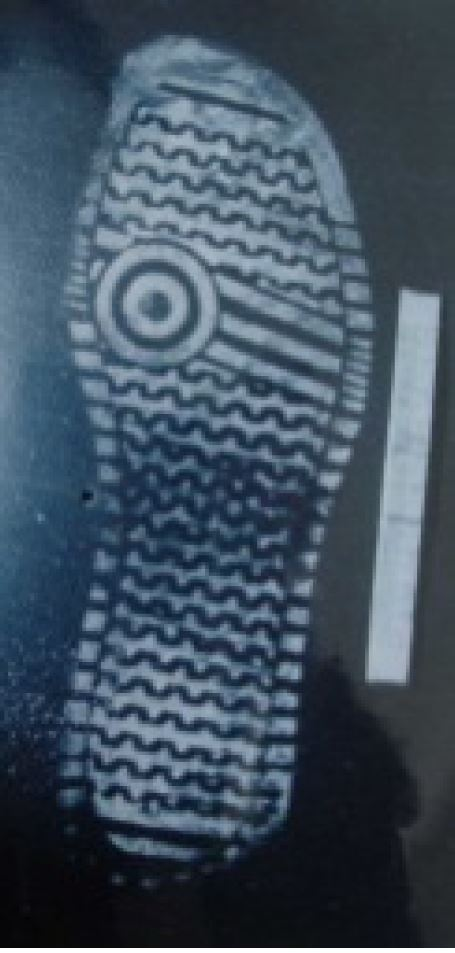
\includegraphics[width=\textwidth]{2/restricted.jpg}
    \subcaption{Example image from a real crime scene dataset excluding low quality images}
    \label{fig:rw:restricted}
  \end{subfigure}
  \begin{subfigure}[t]{0.24\columnwidth}
    \centering
    \includegraphics[width=\textwidth]{2/00025.jpg}
    \subcaption{Example high quality image from the FID-300 database}
    \label{fig:rw:highFID}
  \end{subfigure}
  \begin{subfigure}[t]{0.24\columnwidth}
    \centering
    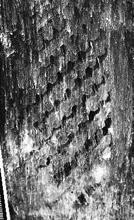
\includegraphics[width=\textwidth]{2/00174.jpg}
    \subcaption{Example low quality image from the FID-300 database}
    \label{fig:rw:lowFID}
  \end{subfigure}
  \caption{Example images of a synthetic \cite{alizadeh2017automatic}, of a restricted \cite{li2014retrieval} and of the FID-300 \cite{kortylewski2014unsupervised} dataset}
  \label{fig:rw:database}
\end{figure}

\par
Morphological Operations, Thresholding and Image Filtering are popular techniques for improving the quality of both kind, realistic and synthetic, of input data.
Morphological Operations, especially Opening and Closing, is used in many cases \cite{wang2014automatic}, \cite{kong2014novel}, \cite{li2014retrieval}, \cite{tang2010footwear}, \cite{wu2019crime}, where Wang et al. \cite{wang2014automatic} uses a synthetic dataset, and other than Wu et al. \cite{wu2019crime} the forensic images are restricted to high quality data.
Wang et al. \cite{wang2014automatic}, Kong et al.  \cite{kong2014novel} and Li et al. \cite{li2014retrieval} use the Morphological Operations to correct inconsistencies after thresholding.
Similar to the previous approaches Wu et al. \cite{wu2019crime} applies the same pipeline on a real forensic dataset.
Tang et al. \cite{tang2010footwear} follow the same principle but instead of thresholding, after Canny edge detection Opening and Closing is used.
\par
To create a binary image and eliminate noise various thresholding techniques are used.
Otsu  \cite{wu2019crime}, \cite{algarni2008novel}, \cite{alizadeh2017automatic}, \cite{kong2014novel} and adaptive thresholding \cite{wang2014automatic}, \cite{li2014retrieval} are two popular algorithms.
Algarni et al. \cite{algarni2008novel} and Alizedah et al. \cite{alizadeh2017automatic} along with Wang et al. \cite{wang2014automatic} published their algorithms for synthetic datasets.
Kong et al. \cite{kong2014novel} and Li et al. \cite{li2014retrieval} tested on restricted, whereas Wu et al. \cite{wu2019crime} developed their approach for real forensic database.
Wang et al. \cite{wang2014automatic} and Wu et al. \cite{wu2019crime} combine thresholding with a grid based approach to calculate exact thresholds for every subarea of the picture.
\par
Another way to eliminate noise is image filtering.
Alizadeh et al. \cite{alizadeh2017automatic} uses a simple Median filter on a synthetic dataset.
Zhang et al. \cite{zhang2005automatic} test on synthetic database as well, and they take advantage of the Partial Differential Equations approach.
In this way the edges are preserved while the background is smoothed according to a controlled curvature motion criteria. 
Katireddy et al. \cite{katireddy2017novel} uses Successive Mean Quantization Transform (SMQT) \cite{nilsson2013smqt} as an only step to enhance the real-life database.
Figure \ref{fig:rw:SMQT} shows the output of the SMQT algorithm on an example image.

\begin{figure}[h]
  \centering
  \begin{subfigure}[t]{0.4\columnwidth}
    \centering
    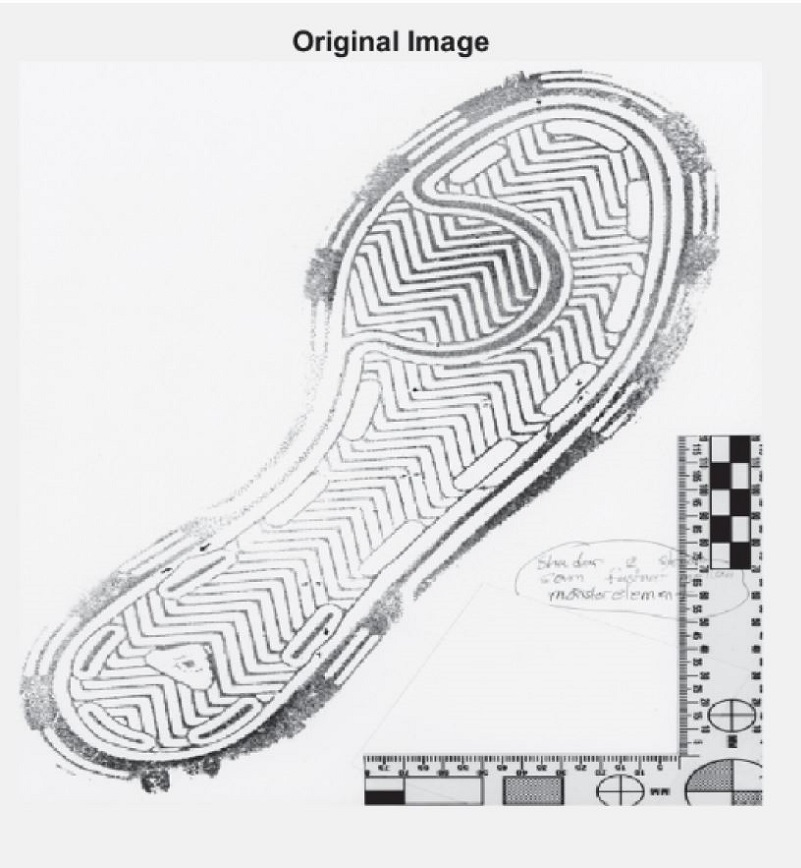
\includegraphics[width=\textwidth]{2/SMQTorig.jpg}
    \subcaption{Example shoeprint impression}
    \label{fig:rw:SMQTin}
  \end{subfigure}
  \begin{subfigure}[t]{0.4\columnwidth}
    \centering
    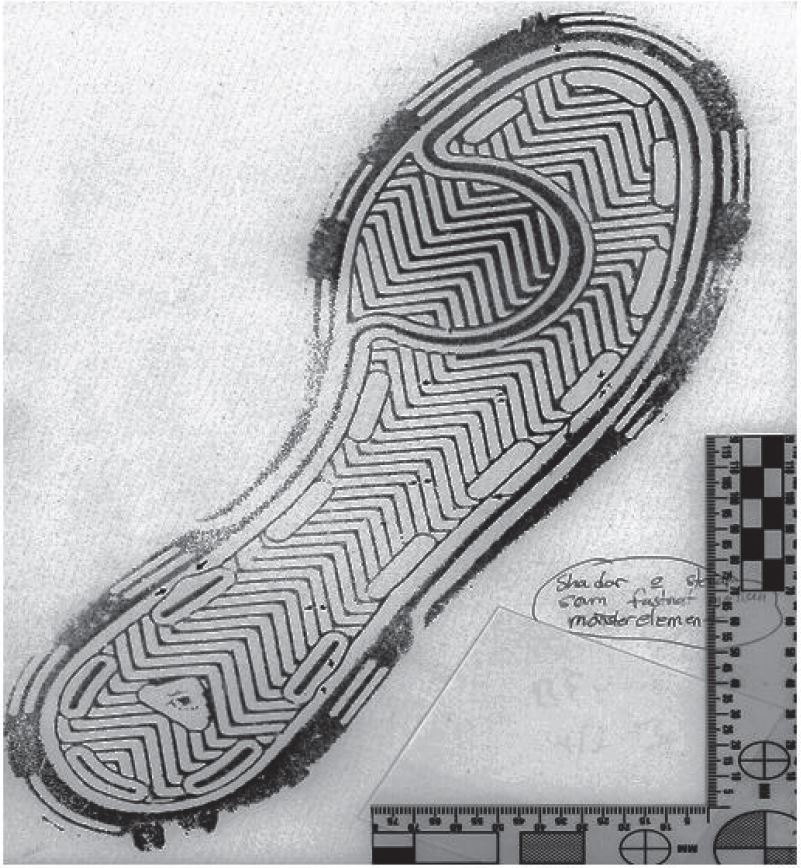
\includegraphics[width=\textwidth]{2/SMQT.jpg}
    \subcaption{Enhanced image with the SMQT algorithm}
    \label{fig:rw:SMQTout}
  \end{subfigure}
  \caption{Example image presenting the enhancement feature of the SMQT algorithm \cite{katireddy2017novel} }
  \label{fig:rw:SMQT} % \label has to be placed AFTER \caption (or \subcaption) to produce correct cross-references.
\end{figure}

\par
Bandpass operators are also used for noise suppression.
The images are converted to the frequency domain where high and low frequencies are eliminated.
Gueham et al. \cite{gueham2007automatic} and Richetelli et al. \cite{richetelli2017classification} utilize this method on a synthetic database.
Li et al. \cite{li2014retrieval} work with a restricted real dataset, where only the lower frequencies are eliminated.
Another frequency based approach was proposed by Katireddy et al. \cite{katireddy2017novel} for real dataset based on Daubechies wavelets
After SMQT enhancement the Daubechies wavelets are used to separate the fore- and background and to remove the noise in the latter.

\section*{Fingerprint Enhancement}

Bandpass and general image filtering is popular in the field of fingerprint enhancement as well.
Zhou et al. \cite{zhou2011adaptive} uses a low- and a highpass filter to eliminate striking frequencies. 
Baig et al. \cite{baig2015enhancement} apply Directional Hilbert transform of Butterworth bandpass to collect the different phase shifts and eliminate the artifacts created by previously thresholding the input.
Wang et al. \cite{wang2014enhanced} decompose the image into four subbands and process them separately, calculating the noise for every subband respectively.
Li et al. \cite{li2012texture} use Fourier transformation combined with Scale Invariant Feature Transform (SIFT) \cite{lowe1999object} to enhance the fingerprint images. 
With SIFT the interesting points in the Fourier domain are found and secured, while the image is filtered to suppress noise and eliminate other inconsistencies.
Jahan et al. \cite{jahan2017robust} apply Fuzzy filtering followed by thinning.
Fuzzy filter is a local method to preserve the edge information and fine line structures while suppressing the noisy background of the input.

\section*{Tattoo Enhancement}

For tattoo enhancement an algorithm from Han et al. \cite{han2013tattoo} was proposed which combines Gaussian filtering with Hysteresis thresholding. 
Hysteresis thresholding is a neighborhood-aware approach where a pixel is labelled when it is above a given low threshold and simultaneously connected to other pixels meeting a higher thresholding criteria.
Acton et al. \cite{acton2008matching} propose to use Active Contour Model to find the boundaries of tattoo images and apply Opening and Closing as well to eliminate small inconsistencies.

\section*{Natural Image Enhnacement}
\par
Along with Signal, especially Bandpass, Filtering, general Image Filtering and Thresholding, Histogram and Color Operations are frequently used for natural image enhancement as well.
Maini et al. \cite{maini2010comprehensive} published a review about natural image enhancing algorithms and defined two main groups of algorithms, Frequency and Spatial Domain Methods.
First, publications utilizing techniques from the former group are discussed, followed by a review of Spatial Domain Methods. 
\par
Xu et al. \cite{xu2016image} combines Bandpass filtering with adaptive thresholding.
Similar to Wang et al. \cite{wang2014enhanced} the image is separated into four subbands, and the threshold is calculated for every image separately.
Sugamya et al. \cite{sugamya2016image} applies Subband Decomposition with two staged Histogram Equalization.
The histogram of the input is equalized globally first, after that it is decomposed into subbands to equalize the values locally for every four generated subimage.
\par
Median Filters are used not only in the domain of shoeprint enhancement \cite{alizadeh2017automatic}, but also for natural image noise suppression.
Apart from Median Filter, Li et al. \cite{li2014rapid} utilize Average and Wiener Filter as well to suppress the occurring noise and to prepare the input for neighborhood based feature extraction.
Feng et al. \cite{feng2011bag} proposed a Bag-of-Words algorithm based on the Gabor wavelets of the input. 
For preprocessing, the Watershed Transform is used.
\par
Histogram Operations are combined apart from Bandpass filtering, like Sugamya et al. \cite{sugamya2016image} propose, also with Thresholding as suggested by Yao et al. \cite{yao2016image}. 
Their approach first separates the histogram of the input into two parts using the Otsu\'s method, then equalizes the histogram of the generated subimages. 
Figure \ref{fig:rw:BHNMT} shows the results of the above algorithm on an example image.

\begin{figure}[h]
  \centering
  \begin{subfigure}[t]{0.4\columnwidth}
    \centering
    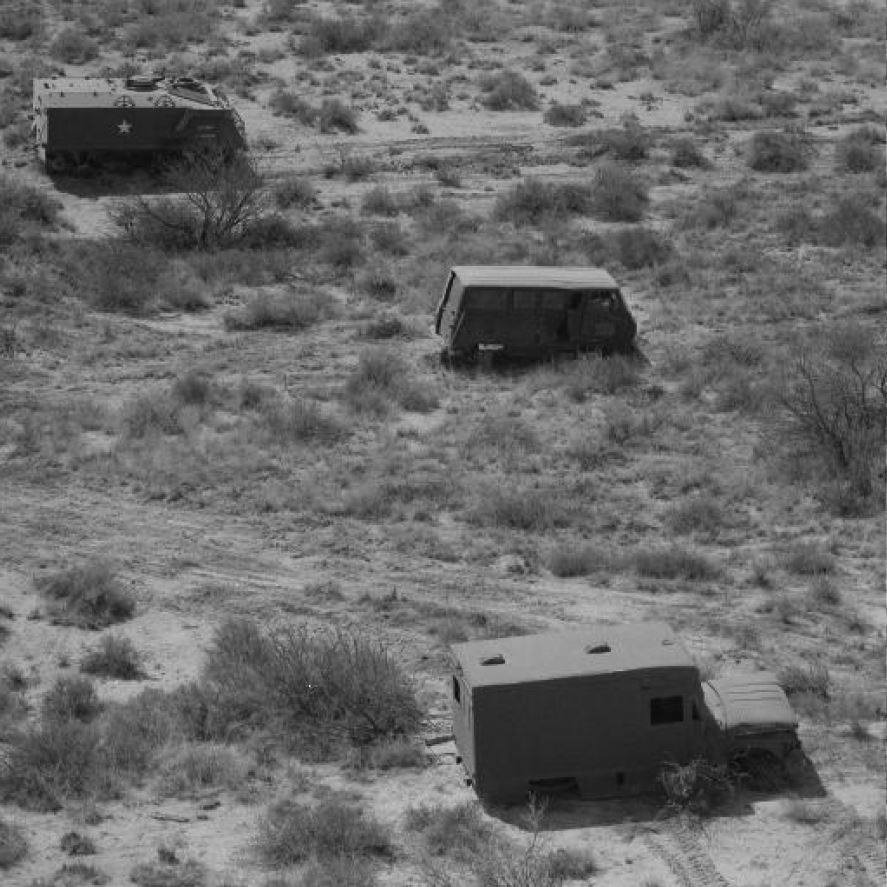
\includegraphics[width=\textwidth]{2/BHNMTorig.jpg}
    \subcaption{Example low-contrast image}
    \label{fig:rw:BHNMTin}
  \end{subfigure}
  \begin{subfigure}[t]{0.4\columnwidth}
    \centering
    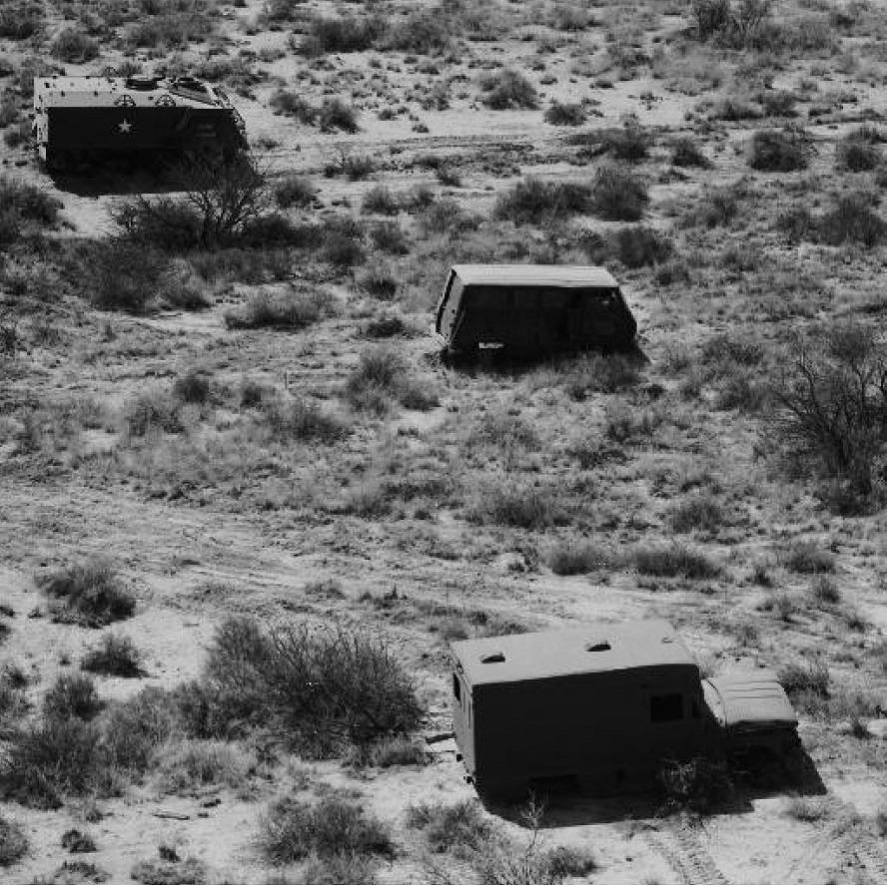
\includegraphics[width=\textwidth]{2/BHNMT.jpg}
    \subcaption{Enhanced image with the histogram thresholding algorithm}
    \label{fig:rw:BHNMTout}
  \end{subfigure}
  \caption{Example image of the enhancement feature of the algorithm proposed by Yao et al. \cite{yao2016image} }
  \label{fig:rw:BHNMT} % \label has to be placed AFTER \caption (or \subcaption) to produce correct cross-references.
\end{figure}

\par
Color processing techniques are widely used for natural image enhancement.
It is applied for image dehazing at low contrast images, \cite{singh2018dehazing} and also for regular noise removal \cite{ren2018joint}, \cite{zhang2016simultaneous}. 
Bhairannawar et al. \cite{bhairannawar2017color} switch from RGB to HSV and use Laplace filter to detect regions with intensity changes. 
During processing the H channel is not modified to prevent color distortion artifacts.
Although color processing is a well researched field with promising solutions, no wider overview of this topic is given in this thesis, since the here used FID-300 dataset provides only grayscale images. 
An example of a shoeprint impression dataset with colored samples is find at \cite{katireddy2017novel}. 

\section{Noise Removal}

Noise Removal methods reviewed in this section are based on estimating the original image and eliminating the deviating features of the data.
One way is denoising through gradient histogram preservation \cite{zuo2013texture}.
The distribution of gradients is estimated on the original image, and the noisy image is adjusted to the calculated values.
An alternative way is to decompose a single image and based on the clear parts, approximate the noisy regions.
Huang et al. \cite{huang2013self} propose a self-learning algorithm that only considers the high frequency parts of the decomposed image.
In \cite{xu2015patch}, \cite{talebi2013global}, \cite{chatterjee2011patch} and \cite{guo2015efficient} images  are separated spatially instead of on the frequency domain, the techniques are based on the idea of non-local means, where the pixels are clkustered according to a given criteria and they are set to the mean of the members belonging to the same cluster.
The difference between the previous algorithms is how they classify the pixels or regions into different classes.
Taleby et al. \cite{talebi2013global} uses an iterative shrinkage strategy. 
Chatterjee et al.  \cite{chatterjee2011patch} group the geometrically similar regions and estimate the noise for every class separately with the Wiener filter, whereas Guo et al. \cite{guo2015efficient} utilize Block Matching to determine cluster memberships. 
Additionally the spatial location is also considered while calculating the mean value in a given class.
The members are weighted according to their distance to the current region.

\section{Image Description}

Similar to the previous Image Enhancement section \ref{sec:rw:ImageENhancement} this part is also subdivided into four domains offering solutions for image description in different areas.
Similar topics are reviewed to gain insight about the powerful descriptors and to consider whether they can be used in the domain of shoeprint enhancement.
Shoeprint descriptors are described first, followed by the fingerprint features.
Finally, at the end of the section tattoo and natural texture descriptors are also reviewed. 

\section*{Shoeprint Descriptors}
\par
Shoeprint Description in varying datasets is an issue in the research of Shoeprint Identification, therefore the properties of the database the given approach was tested on is highlighted for each case.
Signal or frequency domain based image features are popular in both groups of algorithms using synthetic or real samples for testing.
Gabor Transform is used in several applications tested on synthetic \cite{patil2009rotation}, on restricted \cite{kong2014novel}, \cite{li2014retrieval} and on real forensic data \cite{wu2019crime} as well.
Patil et al. \cite{patil2009rotation} propose to use the Radon Transform to determine the dominant direction of structures on the print and to process the aligned image with Gabor Transform.
Kong et al.  \cite{kong2014novel} combined the Gabor features of the sample with Zernike features to describe the shapes in the pattern.
Li et al. \cite{li2014retrieval} suggest to use the histogram extracted in the Gabor transformed domain as descriptors.
In the approach published by Wu et al.  \cite{wu2019crime}, Gabor Filters are combined with Haar Wavelets and Fourier-Mellin Transform to get an integrated, multi-level descriptor. 
There are other publications along that where Fourier-Mellin Transform is proposed for feature description.
Gueham et al. \cite{gueham2008automatic} use the classical Fourier-Mellin pipeline to compare samples of a synthetic dataset.
As Wang et al. \cite{wang2014automatic} state, Fourier-Mellin Transform allow multiresolution matching, so they apply it successfully on synthetic data.
Richetelli et al. \cite{richetelli2017classification} classify synthetic shoeprint impressions by applying Fourier-Mellin Transform following the calculation of Phase Only Correlation (POC) to determine the translative difference between two images in the frequency domain.
Gueham et al. \cite{gueham2007automatic} in another paper suggest to use the basic Fourier Transform before calculating the POC.
Unlike the approach of Gueham et al. \cite{gueham2007automatic}, which were only tested on synthetic images, Kortylewsky et al. \cite{kortylewski2014unsupervised} propose a Fourier Transformation based method for real forensic images.
It is an unsupervised learning approach, where the periodic structures of a shoeprint are compared in the Fourier domain.
Richetelli et al. \cite{richetelli2017quantitative} compares Randomly Acquired Characteristics of shoeprints, e.g. small damages, modifications and stuck objects on or in the shoesole pattern, examining their Fourier descriptor.
Other than Fourier-like transformations, the use of Power Spectral Density was also proposed for a restricted dataset \cite{dardi2009texture}.
It is a descriptor for random, broadbrand signals based on the the frequency and power.
\par
In high quality, so synthetic or restricted datasets shape descriptors are a popular choice for feature extraction.
Algarni et al. \cite{algarni2008novel} suggest to use Hu moments because of its robustness against noise, rotation and resolution.
For restricted databases it is proposed to combine the feature descriptors, Kong et al. \cite{kong2014novel} incorporate Zernike and Gabor features whereas Tang et al. \cite{tang2010footwear} define their own fundamental shapes based on common basic structures on a shoe sole through Hough Line Transform. 
The extracted features are then stored in an Attributed Relational Graph to represent the entire shoeprint image.
\par
SIFT and Harris Detector are popular point descriptors for matching shoeprint images.
Nibouce et al. \cite{nibouche2009rotation} propose to use a four-level Harris and combine it with SIFT on a synthetic database.
Almaadeed et al. \cite{almaadeed2015partial} use the same combination and uses the Hessian Detector additionally for the same purpose in case of restricted real-life datasets.
Another publication \cite{richetelli2017classification} extract the SIFT features from the frequency domain after applying Fourier-Mellin Transformation and POC on the input image.
\par
Kong et al. \cite{kong2017cross}, \cite{kong2019cross} define a descriptor for real database extracting the mid-level features from a Convolutional Neural Network.
Wu et al .\cite{wu2019losgsr} also use machine learning to calculate opinion scores for given matching pairs from real forensic data.
In the learning process manifold ranking is used where he opinions of human experts as well as feature similarities are both incorporated.
Kortylewsky et al. \cite{kortylewski2016probabilistic} developed hierarchical composition for Active Basis Models for the same real database, FID-300, as used in this thesis, and also extended for natural image environments \cite{kortylewski2019greedy}.
Sparse representation was also proposed in \cite{alizadeh2017automatic}, this method, however, was only tested on synthetic data and not on a real forensic dataset.

\section*{Fingerprint Descriptors}
\par
Signal domain representations, because of their robustness against rotation, are attractive not only for shoeprint but also for fingerprint description.
Multi-resolution representation through Gabor expansion was proposed by Bolle et al. \cite{bolle2012fingerprint} to achieve a localized texture descriptor.
Van et al. \cite{van2016fingerprint} use Adaptively Adjusted Modified Finite Radon Transform after Gabor filtering to connect edges and eliminate inconsistencies.
Rida et al. \cite{rida2018palmprint} propose an ensemble descriptor consisting of Gabor filter, Local Binary Pattern, Histogram of Oriented Gradient and Line detector to represent a palmprint impression.
Other than that, Li et al. \cite{li2012texture} suggest to use Directional Filter Banks, where the image is separated into eight directions and every subimage is decomposed into two frequencies via Wavelet Transform. 
\par 
Unlike at shoeprint image representation, in case of fingerprint images several point feature descriptors were proposed.
In \cite{zhou2011adaptive} SIFT features were fused with Hough Transform and Minutiae Information of the fingerprint.
Chen et al. \cite{chen2013hierarchical} also use the Hough Transform and extend it with a hierarchical voting score to improve the matching information available. 
Along  \cite{rida2018palmprint} Ghandehari et al. \cite{ghandehari2012palmprint} recommend to use HOG in a 3-level Gaussian pyramid to estimate the local strength of different types of edges on the image.
Jahan et al. \cite{jahan2017robust} suggest to combine the Minutiae Information with Speeded Up Robust Features and compare them with a Neural Network to find the matching pairs.
\par
According to the following publications, Local Binary Patterns (LBP) are also suitable for fingerprint description.
As mentioned previously, Rida et al. \cite{rida2018palmprint} published a combined feature vector that LBP is also a part of.
Wang et al. \cite{wang2013pixel} modify the usual LBP pipeline with Pixel to Patch sampling to increase the quality of the descriptor without slowing down the calculation.
At Pixel to Patch sampling,  instead of interpolation the weighted average of the neighboring pixels in a given radius is calculated. 
Additionally, the Local Neighboring Intensity Relationships subtracted from their grey-scale information are also considered.
\par
Sparse representations are also used for fingerprint description.
Rida et al. \cite{rida2018palmprint} stores the hybrid features in that way, whereas Shao et al. \cite{shao2013fingerprint} represents predefined fingerprint patches, called dictionary atoms, in a sparse way.

\section*{Tattoo Descriptors}
\par
For tattoo description, three methods are overviewed, which are signal domain features, point descriptors, especially SIFT, and shape features, whereas Kim et al. \cite{kim2015robust} fuses all three of them. 
For local descriptor, the Shape Context Features are used, whereas for global descriptor multi-level SIFT and the Fourier Transform is utilized. 
Acton et al. \cite{acton2008matching} built an Active Contour Model which consists of Haar Wavelet, an HSV histogram and a Fourier Shape Descriptor.
\par
Other than  \cite{kim2015robust}, there are multiple publications available, such as \cite{duangphasuk2013tattoo}, that take advantage of SIFT features for tattoo image description.
It is common to combine them with other shape descriptor to have a more detailed representation.
Han et al. \cite{han2013tattoo} fuse Active Shape Models with SIFT, in \cite{yi2015impact} SURF is added and in \cite{kim2016tattoo} SIFT is extended with the Local Self Similarity measure.
Duangphasuk et al. \cite{duangphasuk2013tattoo} base their approach mainly on shape description and similar to  \cite{kim2015robust} use Shape Context Features for tattoo representation.

\section*{Natural Texture Descriptors}
\par
For natural texture description signal domain features and LBPs are frequently used.
Mistry et al. \cite{mistry2017content}  mix multiple features, mainly color and texture descriptors.
For texture description, Gabor Wavelet and Binarized Statistical Images  \cite{kannala2012bsif} are used simultaneously.
Hatipoglu et al. \cite{hatipoglu2000image} suggest applying Dual Tree Complex Wavelet transform instead of Gabor Wavelet.
Quevedo et al. \cite{quevedo2002description} and Xu et al. \cite{xu2009viewpoint} propose Fractal features, because they are invariant to intensity and scale changes.
Xu et al. \cite{xu2009viewpoint} recommend to use additional multifractal spectrum to achieve robustness against viewpoint changes and non-rigid deformations  
Hayati et al. \cite{hayati2018wirif} and Ahonen et al. \cite{ahonen2009rotation} follow the same principle by incorporating LBP-like features with the frequency domain representation.
Ahonen et al. \cite{ahonen2009rotation} calculate the LBP of the Fourier features of the image, whereas Hayati et al. \cite{hayati2018wirif} use Wave Inference, where the information of multiple different-sized asymmetric neighborhoods is added respectively. 
\par
There are several publications available which use LBPs for texture description, e.g. \cite{guo2012discriminative}, \cite{hong2014combining}, \cite{ahonen2009rotation}, or for texture classification, e.g. \cite{khellah2011texture}, \cite{guo2010rotation}, \cite{zhang2017learning}.
LBP is frequently used also in combination with other techniques. 
In \cite{hong2014combining} based on the covariance matrix additional discriminative features are calculated. 
As mentioned previously, Ahonen et al. \cite{ahonen2009rotation} use the LBP features of the Fourier domain, similarly, in \cite{guo2010completed} LBPs are calculated twice, after separating the input into two components first, into signs and magnitudes, to make the basic LBP rotation invariant as well.
Zhang et al.  \cite{zhang2017learning} propose a learning strategy for adaptively weighting the sign and magnitude LBPs to estimate their contribution in the given area. 
Along the sign and magnitude LBPs, a third modified LBP is also defined, where the local difference vector is determined, in this way robustness against illumination changes is achieved.
In \cite{khellah2011texture}, LBP is calculated on multiple levels.
Another solution for rotation invariance is proposed by Davarzany et al. \cite{davarzani2015scale}. 
In their approach additional circular neighboring radius and a dominant orientation is stored so that scale invariance is also granted.
Li et al. \cite{li2014rapid} process the neighborhood with Rapid Transform, which is robust against cyclic permutation, to achieve the same robustness.
Wang et al. \cite{wang2017local} suggest solving this problem by storing the radial and tangential information instead of the intensity values.
Guo et al. \cite{guo2010rotation} defines "LBPV" instead of LBP, where V stands for variance. 
In their approach the LBP features with high variance are chosen as discriminative, because they indicate high frequency in the related region.
In \cite{bala2016local} it is proposed to calculate Local Texton Patterns, where the Value channel of the HSV input is subdivided into overlapping subblocks according to its content, and the modified LBP is then determined based on those subregions.
Fadaei et al. \cite{fadaei2017local} published a similar approach called Local Derivative Radial Patterns.
Instead of binary coding, a multi-level coding is used in four directions, and the differences between neighbors are weighted additionally.
Chahi et al. \cite{chahi2018local} define Local Ternary Patterns which store the directional patterns explicitly.
\par
In \cite{kannala2012bsif}, a new LBP similar descriptor is defined called Binary Statistical Image Feature (BSIF) which is also proposed to use by Crossier et al. \cite{crosier2010using}. %REVIEW. 
In BSIF, pre-learnt filters are used and the responses are stored in the feature.
It can handle large intra-class variance when used for classification, however, it varies greatly when the scale changes. 
For this reason, Crossier et al. \cite{crosier2010using} suggest calculating the features on multiple resolutions in order to gain scale invariance as well.
\par
Varied Local Edge Pattern Descriptors (VLEP) \cite{yan2016edge} are used to represent edge information.
Every pixel of an edge is described by the angle and by the magnitude of the gradient, which stand for edge direction and strength, respectively. 
Wang et al. \cite{wang2018using} extend the feature to be scale invariant by combining two or more modified VLEPs, one calculated on a different scale and another calculated on different scale and resolution.

\chapter{Methodology}

\par
In this chapter three different algorithms for shoeprint enhancement are introduced, the first one is based on feature learning, the second one uses image filtering and the third one builds a Fourie-Mellin based noise model and applies the non-local means algorithm as well.
As mentioned earlier the testing data of already published algorithms varies, thus it is difficult to make an estimation about their performance on the FID-300  \cite{kortylewski2014unsupervised} dataset.
For that reason three prototypical application are developed and evaluated in this thesis, and the one with most promising results is further analyzed.
The goal of this chapter is to give an overview about possible directions of development and to present the working pipeline and the implementation details of the proposed methods.
\par
A measure for image quality is the signal to noise ratio, a high value indicates high quality image, where the content is clearly visible, a lower value stands for low quality where the noise suppresses the content of the image.
In case of forensic images, the outlines of the shoeprint pattern represent the content, the information of the image, and clutter or additional objects in the background cause noise. 
The three proposed algorithms attempt to enhance the shoeprint impressions by increasing the signal to noise ratio of the input, thus increasing the contrast between the fore- and the background of the image.
Two ways are considered to increase the quality of a given input, namely, first, to find and enhance the information regardless of the properties and presence of noise, or second, to suppress any kind of noise preserving the information. 
The first algorithm focuses on finding the shoeprint pattern in varying conditions, the second one filters noise and the last one combines both of them by suppressing the noise with the calculated noise model and enhancing shoeprint pattern information using the non-local means method.

\section{Feature Learning for Shoeprint Detection}

\par
To find the shoeprint pattern in an input regardless the noise a robust and discriminative descriptor is defined.
Since the noise and other inference is highly variable in real-life settings, the impressions from the same shoe differ depending on the circumstances causing high intra-class variance.
Because of that a discriminative feature learning algorithm is proposed based on the work of Guo et al. \cite{guo2012discriminative}.
With the proposed adaptive feature selection, it is possible to learn the discriminative features of a texture and to adjust the selection process according to a given set of reference images of the same texture, according to the versatile appearance of impressions deriving from the same shoe sole.
While training multiple samples of the same texture captured in different circumstances are processed and the features selected on the single images are summarized in the feature pool.
\par
The feature learning algorithm proposed in \cite{guo2012discriminative} was developed originally to find a discriminative feature set for several texture images from a wide database, from \cite{ojala2002outex}, \cite{dana1999reflectance}, \cite{boland2001neural}, \cite{jantzen2005pap} and \cite{brahnam2007introduction}, but in this project no such dataset is available since only a subset of samples from FID-300 are used for learning. 
The FID-300 \cite{kortylewski2014unsupervised} dataset consists of 300 real-life forensic samples and 1175 reference samples, thus not every reference sample has a corresponding real impression, and the majority of reference images with existing corresponding real samples have only one or two examples for real impression in the database.
Since the feature learning algorithm requires multiple representations for the same texture a shoe sole with the highest amount of real-life samples is chosen as training set.
It contains six real-life shoeprint impressions and their reference image. 
Since there is no pixel wise labeled data in the FID-300 dataset available, the samples chosen for training were labeled manually by comparing the sample images to their reference and marking all pixels which are part of the shoeprint pattern.
Figure \ref{fig:pe:mask} shows two example images. 
The black regions of the mask show the shoeprint information whereas the white pixels indicate the background.

\begin{figure}[h]
  \centering
  \begin{subfigure}[t]{0.24\columnwidth}
    \centering
    \includegraphics[width=\textwidth]{3/00009.jpg}
  \end{subfigure}
  \begin{subfigure}[t]{0.24\columnwidth}
    \centering
    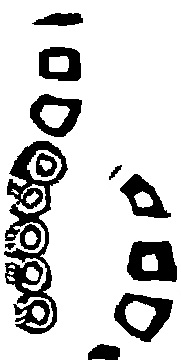
\includegraphics[width=\textwidth]{3/00009_mask.jpg}
  \end{subfigure}
  \begin{subfigure}[t]{0.24\columnwidth}
    \centering
    \includegraphics[width=\textwidth]{3/00025.jpg}
  \end{subfigure}
  \begin{subfigure}[t]{0.24\columnwidth}
    \centering
    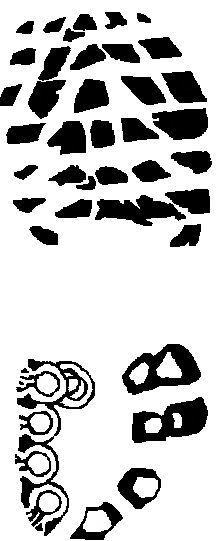
\includegraphics[width=\textwidth]{3/00025_mask.jpg}
  \end{subfigure}
  \caption{Examples from FID-300 \cite{kortylewski2014unsupervised} dataset chosen for three-layered learning and their corresponding manually labelled masks.}
  \label{fig:pe:mask}
\end{figure}

\par
In the work of Guo et al. \cite{guo2012discriminative} a three-layered Local Binary Pattern (LBP) feature learning algorithm is introduced for natural texture description, the schematic workflow the algorithm is shown on Figure \ref{fig:pe:workflow}
They utilize on feature selection where only the discriminative descriptors are chosen and propagated further.
In the first layer the samples of the same textures are examined separately.
Robustness is granted by selecting those features that describe the majority of a texture on the given sample.
This is done by finding the frequently appearing descriptors and ignoring the rare ones since they are more sensitive to noise.
The descriptors of the given texture are selected in the order of their frequencies, starting with the most frequent one.
If the already selected descriptors cover a bigger region of the original texture than a given threshold, the selection process terminates and the chosen descriptors are propagated for the next level.

\begin{figure}[h]
  \centering
  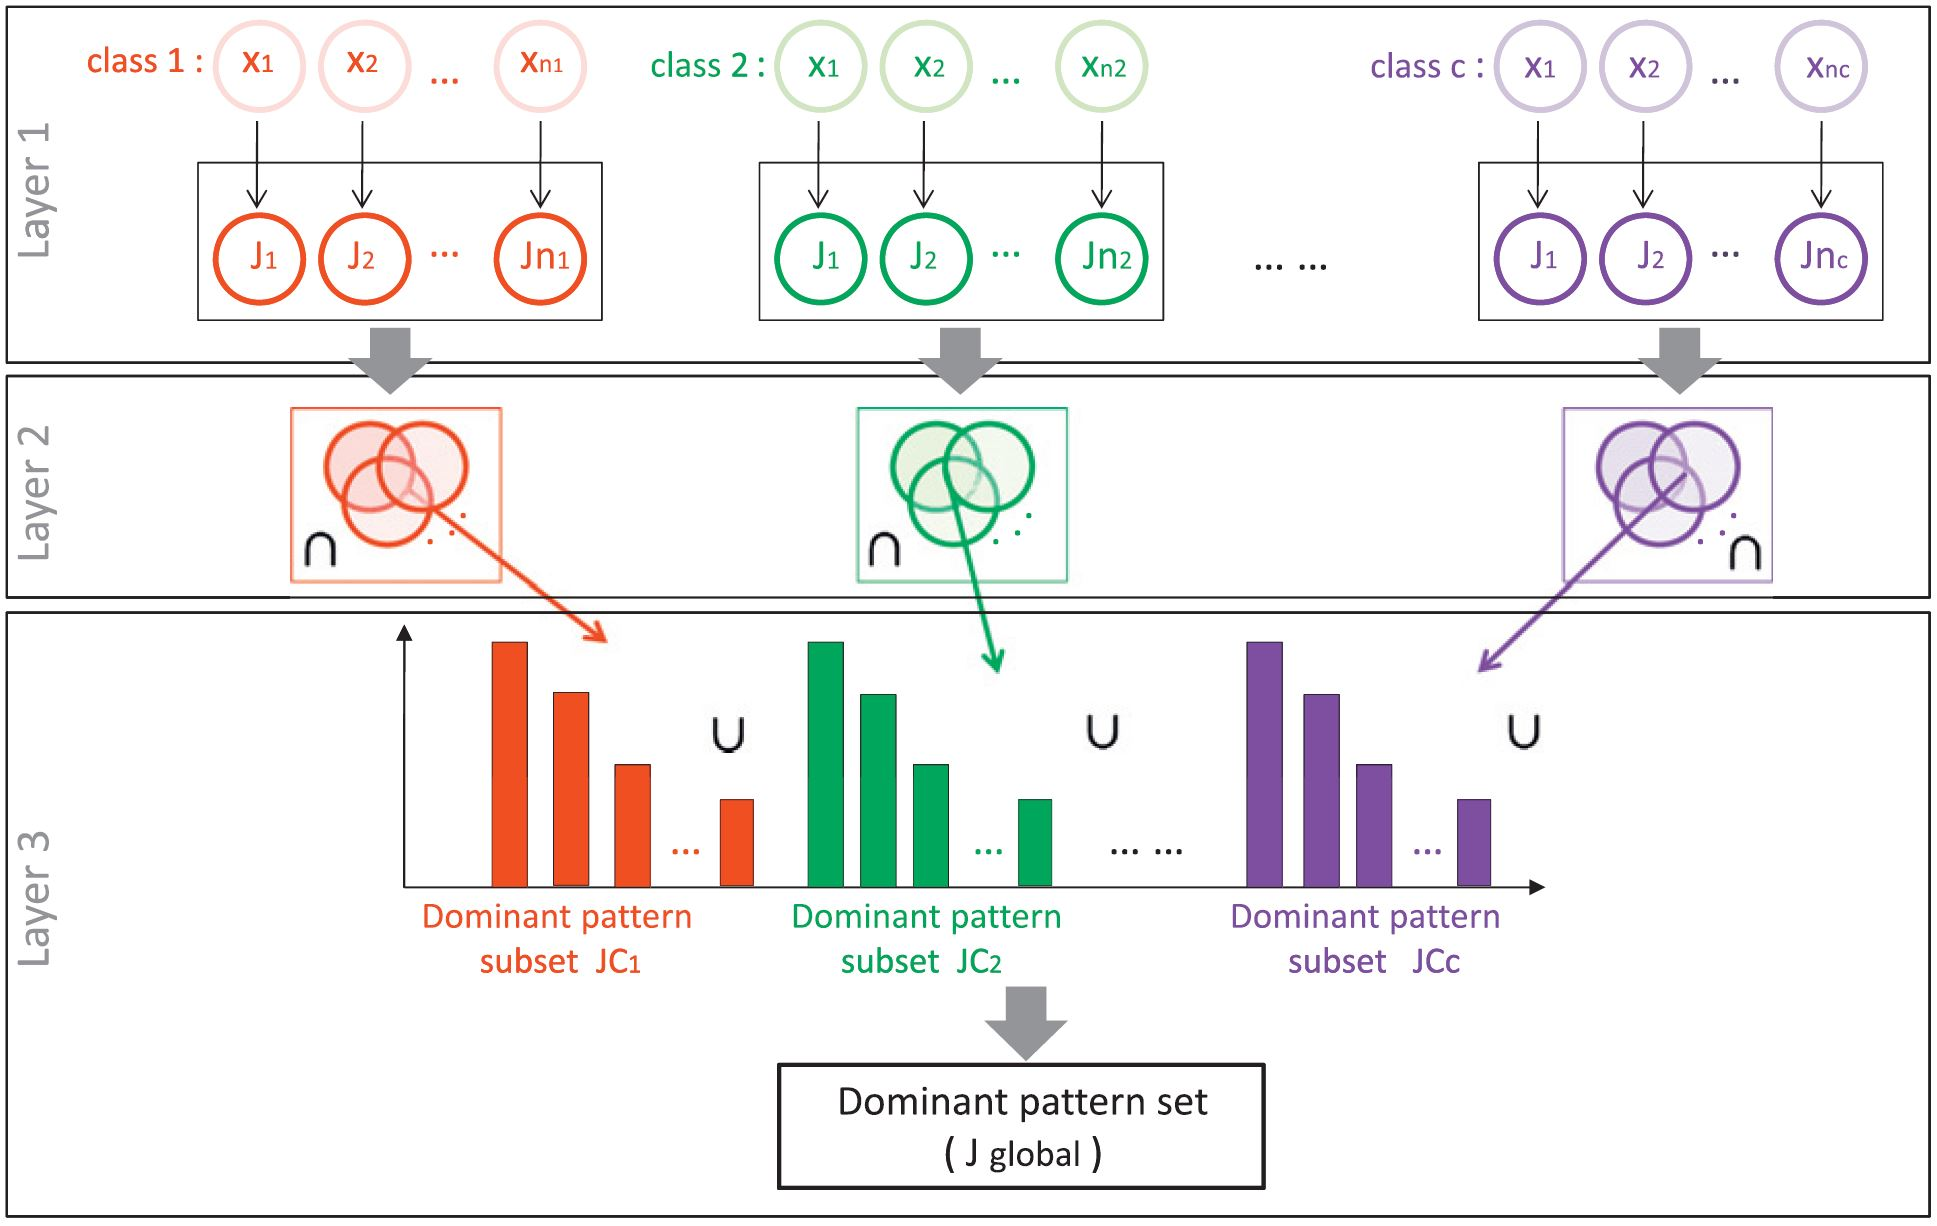
\includegraphics[width=\textwidth]{3/workflow.jpg}
  \caption{The workflow of the three-layered feature learning algorithm  \cite{guo2012discriminative}.}
  \label{fig:pe:workflow} % \label has to be placed AFTER \caption (or \subcaption) to produce correct cross-references.
\end{figure}


\par
Guo et al. \cite{guo2012discriminative} proposed their algorithm for LBP features, and since it is a popular descriptor for natural textures \cite{hong2014combining}, \cite{ahonen2009rotation} and fingerprints \cite{wang2013pixel}, \cite{rida2018palmprint}, LBP is chosen to be a candidate descriptor for shoeprint detection.
In the research of shoeprint identification both frequency based feature descriptors, such as Fourier-Mellin Transform \cite{wu2019crime}, \cite{gueham2008automatic}, and SIFT \cite{nibouche2009rotation}, \cite{richetelli2017classification} were already proposed, thus these are also selected for feature learning.
Therefore along LBP, the feature learning algorithm is also implemented for Fourier-Mellin and SIFT, but the selection process follows the same steps as proposed by Guo et al. \cite{guo2012discriminative}.
For the Fourier-Mellin calculation the descriptors are extended by mirroring the edges to have a uniform-sized, 5x5, descriptor in all cases.
For LBP features two different settings are considered, one with a radius of 3 and 12 sample points and one with a radius of 5 and 24 sample points.
These parameter settings were determined experimentally and their performance is discussed in the following chapter.
\par
An easy way to determine the frequency  of one descriptor is to count the number of complete matches with every other descriptor within one sample.
This method, however, results in high amount of descriptors with little number of occurrence.
Consequently, a similarity measure is used for all three candidate features. 
As similarity measure histogram correlation is used for LBP, matcher called Brute-Force is applied for SIFT and the Fourier-Mellin features are evaluated using the correlation coefficient proposed  in \cite{gueham2008automatic}.
Brute-Force compares one feature to every other features of the image and sets the closest one as match storing the distance value between them.
The correlation coefficient proposed by Gueham et al. \cite{gueham2008automatic} is given as follows:
\[ corr(FM_{1},FM_{2}) = \frac{\sum\limits_{m}\sum\limits_{n}(FM_{1mn}-\overline{FM_{1}})(FM_{2mn}-\overline{FM_{2}})}{\sqrt{(\sum\limits_{m}\sum\limits_{n}(FM_{1mn}-\overline{FM_{1}})^2)(\sum\limits_{m}\sum\limits_{n}(FM_{2mn}-\overline{FM_{2}})^2)}}  \]
\label{FMcorr}
where $FM_{1}$ and $FM_{2}$ are two Fourier-Mellin Features to compare and $\overline{FM_{1}}$ and $\overline{FM_{2}}$ are the mean values of the corresponding features.
If the similarity value reaches a predefined threshold the two descriptors are considered the same and the counter for the frequency of the given feature is increased.
The experimentally determined threshold for similarity is  90\% for LBP histogram correlation, 300 for the maximal distance of two SIFT features and higher correlation than 1.4 between two Fourier-Mellin descriptors.
\par
Guo et al. \cite{guo2012discriminative} suggest a threshold based on the area the selected features cover on the original image.
The selection of threshold is crucial; if it is too high, less robust descriptors with low frequency are also selected, when the threshold is too low, only the most frequent descriptors are considered and valuable details of the texture are ignored.
The parameter settings are determined experimentally and every Fourier-Mellin feature is propagated which occures at least 10 times on the shoeprint pattern.
However, this criteria is altered in the case of LBP and SIFT to eliminate by noise distorted descriptors as follows.
Features are firstly extracted both from the fore- and the background of the samples, where the foreground contains the exact shoeprint pattern and the background is the noisy ground where the shoeprint is lying. 
After this, to achieve high inter-class distance between shoeprint pattern and noise, frequent descriptors of the noise are determined and all of them are eliminated from the pattern descriptors.
The same similarity measures defined above are utilized to determine the frequency of the noise descriptors and to eliminate them from the pattern descriptors.
If the histogram correlation between two LBP noise features is higher than 90\% or the matching distance between two SIFT descriptors is lower than 300 the counter for frequency of the given noise feature is increased.
These thresholds and the following parameter setting are determined experimentally and the noise similarity criteria is set to be the same as the required similarity between descriptors of the shoeprint patterns.
Afterwards the most frequent noise descriptors are determined, occurring at least 100 times among LBP and at least 10 times among SIFT features.
All LBP and SIFT shoeprint descriptors are eliminated which have higher than 90\% correlation with or have smaller than 250 distance to any dominant noise descriptor.
The remaining pattern descriptors are propagated to the next level. 
\par
The following two layers work according to Fisher's Separation Criteria, the second layer aims to minimize intra-class variance, whereas the third layer ensures maximum inter-class distance. 
The second layer gathers all selected descriptors from the previous layer of the same texture, that are the extracted shoeprint pattern features, on different samples and intersects those sets.
The assumption is that the same texture have similar properties under varying circumstances.
During this process, features are selected that occur in every sample of the given texture.
If there is a feature in every sample of the same texture with a high enough similarity the feature is chosen and added to the final descriptor pool.
The same similarity measures defined in the first layer are used for feature comparison, the thresholds for similarity are determined experimentally.
If the correlation between two LBP descriptor is higher than 90\%, the distance between two SIFT features is smaller than 450 and the correlation between two Fourier-Mellin features is higher than 1.4, the feature is chosen and added to the final set of descriptors.
\par
In the last, third layer representation capability is ensured.
This layer merges all remaining features from the second layer into one set to create a dominant feature pool.
In the second layer a feature set for a given texture is created based on the extracted descriptors from all samples of the same texture.
In the third layer those feature sets of every occurring textures are collected and united.
For the purpose of this prototypical implementation only the first two layers are used, because only one texture class, "shoeprint", is defined.
Since the noise pattern is unique to each sample and seemingly does not follow any regularities across them, descriptors for shoe patterns are only learned.
That means, that only one texture set is available, therefore no merging across multiple textures is needed.
\par
At the end of the learning process a descriptor pool is created.
The shoeprint area of a new input is determined based on those learnt features using the same comparison techniques as in the learning phase.
The descriptors of the input image are determined similarly as in the training phase.
For every pixel of the input a descriptor is calculated, in case of Fourier-Mellin transform the borders of the input are extended by mirroring.
The output image is calculated by comparing the descriptors of the input with the ones in the descriptor pool.
In case of LBP and Fourier-Mellin features the correlation value is written into the resulting image which is normalized at the end of calculation.
The result image of the SIFT feature comparison is binary, it is set to one if the descriptor of the corresponding pixel has a smaller distance than 200 to any descriptor from the learned set.
This distance is determined experimentally, its influence on the resulting image is discussed in the following chapter.


\section{Fully-Automated Noise Elimination}

\par
Similar to the previous method the main goal is to distinguish between noise and pattern, but this time instead of finding pattern regardless of the noise, the noise is suppressed first and the information is enhanced afterwards.
The method proposed in this chapter has three main steps, first the noise is suppressed, after that the shoeprint pattern is enhanced and the result image is generated lastly by thresholding.
A similar pipeline, namely to filter the shoeprint image first and to apply thresholding afterwards, is  often used as a preprocessing step for shoeprint matching \cite{alizadeh2017automatic}, \cite{wang2014automatic}, \cite{li2014retrieval}, \cite{kong2014novel}.
Katireddy et al. \cite{katireddy2017novel} propose to enhance shoeprint impressions using Successive Mean Quantization Transform (SMQT).
In the presented algorithm those two approaches are combined by adding an enhancement step between filtering and thresholding.
In this way the noise is suppressed first, so that SMQT affects the relevant, shoeprint pattern, area, and the pipeline is closed with thresholding to generate the binary image and to eliminate remaining noise parts.
The workflow of the entire algorithm is shown on Figure \ref{fig:fans:workflow}.

\begin{figure}[h]
  \centering
  \includegraphics[width=\textwidth]{4/flow.jpg}
  \caption{The workflow of the fully automated noise suppression algorithm.}
  \label{fig:fans:workflow} % \label has to be placed AFTER \caption (or \subcaption) to produce correct cross-references.
\end{figure}

\par
The first part of the algorithm is responsible for noise suppression.
Two filters proven to be effective in natural image noise elimination are combined, these are Wiener filter \cite{li2014rapid}, \cite{chatterjee2011patch} and Bilateral filter \cite{zhang2016simultaneous}, \cite{huang2013self}.
As Li et al. \cite{li2014rapid} state, Wiener filter is among the most popular techniques in the topic of noise reduction, even though it does not reconstruct the signal data it only suppresses the noise component.
Wiener filter works in the signal domain, where it estimates the original image based on the cluttered input, in this case based on the noisy real-life shoeprint sample. 
The filter is given by following Equation \cite{Win}:
\[ G(u, v) = \frac{H^*(u,v) P_s(u, v)}{\mid H(u,v)\mid ^2 P_s (u, v) + P_n (u, v)}  \]
where $H(u,v)$ stands for the Fourier Transform of the point-spread function, $P_s (u,v)$ denotes the power transform of the signal, which is the Fourier Transform of the signal autocorrelation and $P_n(u,v)$ expresses the power spectrum of noise, which is the Fourier Transform of the noise autocorrelation.
The performance of the filter depends on the quality of $P_s$, on the estimated appearance of the original image.
In this method the estimation is made based on the entire input image, because no further information, for example a mask about the shoeprint  area, is available.
However, this also means that the estimation is less accurate than using an exact representation of the shoeprint area, thus the performance is lower \cite{chatterjee2011patch}.
To apply the Wiener Filter correctly the input image is normalized first to the range of 0 to 1.
For the Point Spread Function an image of size 5x5 is set.
The balance parameter is 1100 which sets the ratio between information adequacy and prior adequacy, those parameters control frequency increment and decrement respectively.
The parameter settings are determined experimentally and set a smaller kernel size, thus less aggressive filtering, intentionally.
As mentioned above the estimation about the appearance of original image is limited, since the original shoeprint impression without noise is not available.
Therefore it is possible that apart from suppressing noise, the shoeprint is also damaged.
With smaller kernel size the noise is less blurred but in exchange the shoepattern information is preserved.
Similar to the Wiener Filter Bilateral Filter is also used for smoothing the image.
Since it considers the weighted average of neighboring pixels, it preserves the edge information which is crucial to prevent blurring on the shoeprint pattern \cite{elad2002origin}. 
The kernel size of the Bilateral Filter is 5x5 which was determined experimentally and is based on the same idea like the parameter settings of the Wiener filter.
A bigger kernel size results in more blurred image background, however, it is not able to preserve the fine-lined foreground area, since the bigger neighborhood outweights the small lines occurring in the filter window.
For that reason a smaller kernel is chosen, to avoid the possible blurring on the shoeprint area.
When both images are calculated the difference between them is propagated.
In this way the blurring effect is strengthened in the background while the outlines of the shoeprint patterns are preserved.
With the combination of both filtered images, the effect of the Wiener and Bilateral filters is amplified, the little blurring caused by the small filter kernels is added in the background while the foreground stays undamaged.
\par
For enhancement Successive Mean Quantization Transform (SMQT) is used \cite{nilsson2013smqt}.
The method was already proposed for shoeprint enhancement by Katireddy et al. \cite{katireddy2017novel}, however, their evaluation dataset  is not publicly available, thus no complete reconstruction of their algorithm is possible.
SMQT is recursive algorithm working on subsets of the entire data which splits the given set into two parts in every recursion level depending on the current value being smaller or bigger than the mean of the entire subset.
In every recursion level the data, in this case the shoeprint sample, is separated into two parts, and it is noted which pixel is under (0) and which one is above (1) the current mean.
The algorithm then recursively continues on both subgroups of the image, splitting and noting the relative value again for every pixel.
Note that the pixels in the same subgroup does not have to be neighboring, the clustering is solely based on the pixel value.
The recursion stops if the predefined depth is achieved.
To finish the transformation the noted cluster values of the pixels are examined.
Along the levels of the recursion a sequence of ones and zeros are registered for every pixel.
As a last step this sequence is considered as a binary number and its decimal value is written into the corresponding pixel.
SMQT works based on the similar principle as Histogram Equalization.
Because of the successive partitioning, the pixel values are spread on the range of the depth of the recursion.
In this way the structure of the data is exposed.
\par
Because of time efficiency, a speeded up version is implemented.
In the first step a table of occuring values on the image is created where the zeroth column corresponds the pixel value of 0, the first column stands for pixel value of 1 and so on.
In the first row of the table, the frequency of the given value is noted, that is the number of pixels having the value which the column corresponds with.
In the second row the sum of frequencies up to the current column is stored.
The third row represents the sum of all elements until the given column.
Since the entries are ordered, if the subgrouping starts, the values belonging to the same cluster will be neighboring columns.
Figure \ref{fig:fans:table} shows the first eight columns of the occurrence map of an example image.
This table eases the calculation of mean value for every level of the SMQT algorithm.
For the mean calculation the sum of all pixels is divided by the number of pixels, which is stored in the third and second row of the table respectively. 
To calculate the mean value of one subgroup two columns of the table are considered, the one before the first column of the subgroup and the last one in that given group.
The values are first corrected by substracting the elements of the former from the latter, and then dividing the third row with the second one the average value of the group is determined.
This correction is needed to eliminate the offset in the table, skipping this step the mean of every pixels having lower or equal value than the biggest element of the given subgroup is calculated.
When the occurrence map is ready the recursion starts, the mean of the given subgroup is determined and the occurrence map is split into two parts according to the pixel value of the given column being bigger or smaller than the mean value. 
Every column of the table have a binary code which is created during the recursion.
In the first level the first digit of the code is written, in the second level the second digit etc., the length of this code is the same as the predefined depth of the recursion.
If a pixel value is smaller or equal to the calculated mean of the given cluster a zero is written into the belonging binary code, and a 1 is recorded if it is bigger.
The manually set depth of the recursion is 8, in this way when the final binary codes are converted to a decimal number a range of 0 to 255 is covered.
\begin{figure}[h]
  \centering
  \begin{subfigure}[t]{0.09\columnwidth}
    \centering
    \includegraphics[width=\textwidth]{4/21/00021.jpg}
  \end{subfigure}
  \begin{subfigure}[t]{0.9\columnwidth}
    \centering
    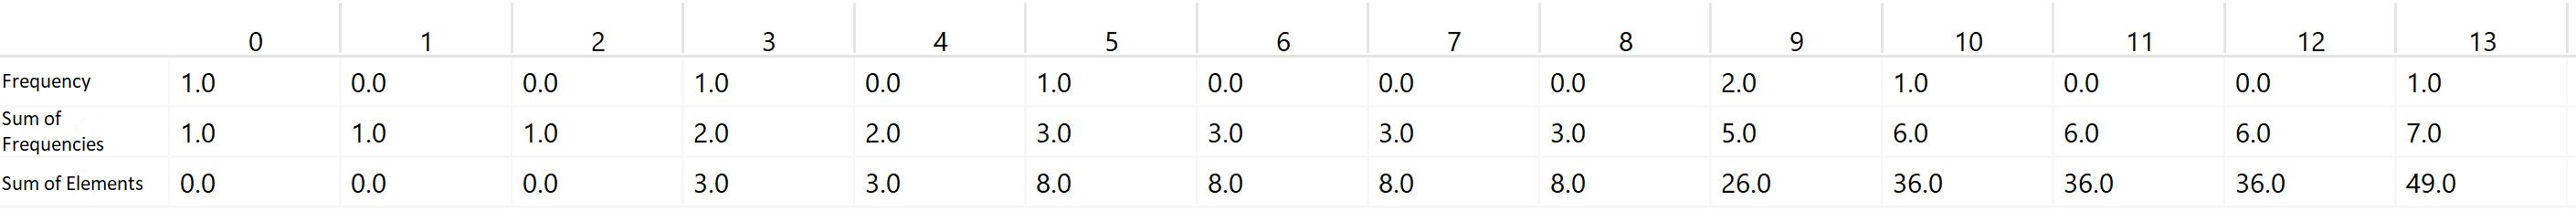
\includegraphics[width=\textwidth]{4/table.jpg}
  \end{subfigure}
  \caption{The first 8 columns of the occurrence map. The header of the table represents the possible pixel values }
  \label{fig:fans:table} % \label has to be placed AFTER \caption (or \subcaption) to produce correct cross-references.
\end{figure}
\par
The last part of the application is the postprocessing step where the input is converted into a binary image and inconsistencies and remaining noise are eliminated.
When binarizing footprint images Otsu's technique \cite{algarni2008novel}, \cite{alizadeh2017automatic}, \cite{wu2019crime} or adaptive thresholding \cite{wang2014automatic} is used frequently.
However in the proposed approach a local thresholding technique, called Niblack Binarization Method (NBM) \cite{niblack1985introduction} is preferred.
There are several publications available \cite{som2011application}, \cite{athimethphat2011review}, which prove that global methods, such as Otsu Thresholding \cite{otsu1979threshold}, is less feasible as their local counterparts.
Although the studies mentioned were carried out on text documents with varying image quality, the two domains are considered as familiar since they both aim to find fine line structures on a cluttered background.
Furthermore, Saxena et al. \cite{saxena2019niblack} also state that NBM is one of the most powerful thresholding methods, outperforming the global and some local techniques as well. 
NBM  is calculated as follows \cite{saxena2019niblack}:
\[T_d = m(x,y) + k * s(k, y)\]
where $m$ and $s$ stands for mean and standard deviation in the given area respectively and $k$ is a configuration variable which is given manually. 
In this thesis the window size is the same as the size of the Wiener Filter, 5x5, and the regularization parameter $k$ is set to 0.5 which values were determined experimentally.
\par
There is, however, one disadvantage of local binarization and that is local window size.
Since for every subwindow a new threshold is calculated NBM tends to generate salt and pepper noise on more homogeneous, e.g. background of the shoeprint pattern, area.
For that reason two other postprocessing methods are also implemented based on the connected components of the image.
They are extracted considering 8-neighborhood, so diagonal connectivity is also considered.
The first postprocessing step eliminates short lines on the image, based on the assumption that the outlines of the shoe pattern build longer, coherent edges.
The second one deletes all remaining open structures unless the length is higher than a given threshold bigger than the one given in the previous method.
Those two heuristics are based on two observations, first,  when there is no shoepint impression region in a NBM subwindow the edges of the remaining clutter and binarization artifacts are generated.
Second, since NBM concentrates on the contours, if the complete structure of a pattern element is found a closed line structure is extracted.
It is possible, however, that an open line structure is generated,  if only parts of the shoeprint are visible or identified correctly.
For that reason, only a subgroup of open lines, the ones that are shorter than a threshold, is eliminated.
It is possible to set the thresholds of the two postprocessing steps to the average size of every region, however, experimental results show that such strong criterion eliminates shoe pattern lines as well.
For that reason two experimentally defined, manually set thresholds are used, they are set to 50 and 60 respectively for every test image.
If an open line structure is found which overall size is smaller than 60 it is deleted.

\section{Shoeprint Enhancement with Non-Local Means}
\par
Since noise tends to appear both on the fore- as well as on the background region, a semi-automated algorithm is introduced in this section, where user input about the noise is expected and based on that information a noise model is calculated.
As mentioned earlier filtering the noise first and using a thresholding method to enhance a shoeprint impression is widely used as preprocessing step for shoeprint matching \cite{alizadeh2017automatic}, \cite{wang2014automatic}, \cite{li2014retrieval}, \cite{kong2014novel}.
Similar to that pipeline, the proposed algorithm has two main steps.
First, the noise is eliminated in two stages, in the first step the background and the foreground, the shoeprint impression, is separated to mask the area of the former one.
After that the the foreground is filtered in the frequency domain to suppress  the noise covering that area.
Second, the shoeprint pattern is enhanced, by extracting the edges and applying the non-local means method, and binarized finally.
Instead of only noise filtering a full separation between fore- and background is possible, because according to the user input a detailed background and noise model is built.
In this way it is possible to mask the noise in the calculated background area instead of just suppressing it with filtering.
Furthermore, the masking does not modify the foreground area, so no shoeprint pattern information is distorted, which is not guaranteed when using a filter on the whole input sample.
As a first step of algorithm, the user has to select a pixel in the background area where there is no pattern information,no foreground, in the neighboring area.
The full pipeline is shown on Figure \ref{fig:sans:workflow}.

\begin{figure}[h]
  \centering
  \includegraphics[width=\textwidth]{5/flow.jpg}
  \caption{The workflow of the semi-automated noise suppression algorithm.}
  \label{fig:sans:workflow} % \label has to be placed AFTER \caption (or \subcaption) to produce correct cross-references.
\end{figure}

\par
Based on the user input the background area is determined according to the Fourier-Mellin features \cite{sheng1986circular}.
Fourier-Mellin features were already used for shoeprint description in both synthetic \cite{gueham2008automatic} and real \cite{wu2019crime} datasets, however, in this algorithm it is used for noise description.
This decision is based on the observation that although the noise varies among samples, there are dominant features within one image which describe the majority of the clutter on a large part of the testing images.
The varying appearance of noise is illustrated on Figure \ref{fig:sans:noiseIll}, comparing the background of the images there is little or no similarity between the samples, however, within one sample dominant patterns are recognizable.
To prepare the descriptor for the variance of the noise, three-different sized samples are extracted around the point determined by a user input.

\begin{figure}[h]
\centering
  \begin{subfigure}[t]{0.19\columnwidth}
    \centering
    \includegraphics[width=\textwidth]{5/noiseIll/00009.jpg}
  \end{subfigure}
  \begin{subfigure}[t]{0.19\columnwidth}
    \centering
    \includegraphics[width=\textwidth]{5/noiseIll/00017.jpg}
  \end{subfigure}
  \begin{subfigure}[t]{0.19\columnwidth}
    \centering
    \includegraphics[width=\textwidth]{5/noiseIll/00025.jpg}
  \end{subfigure}
  \begin{subfigure}[t]{0.19\columnwidth}
    \centering
    \includegraphics[width=\textwidth]{5/noiseIll/00204.jpg}
  \end{subfigure}
  \begin{subfigure}[t]{0.19\columnwidth}
    \centering
    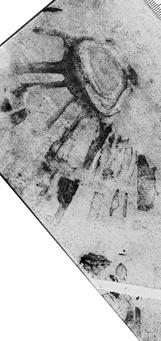
\includegraphics[width=\textwidth]{5/noiseIll/00239.jpg}
  \end{subfigure}
\caption{Example images from the FID-300 dataset. The noise varies across the images, but there are dominant structures within one sample.}
\label{fig:sans:noiseIll}

\end{figure}
\par
Fourier-Mellin features are scale, rotation and translation invariant descriptors and are calculated according to the following equation \cite{kazik2011visual}:
\[\mathcal{M}_f(u,v) = \frac{1}{2\pi} \int_{0}^{\infty}\int_{0}^{2\pi} f(r, \theta)r^{-ju}e^{-jv\theta}\mathrm{d}\theta\frac{\mathrm{d}r}{r}\]
where $u$ and $v$ are the Mellin and the Fourier transform parameter respectively.
If the image is translated, the Fourier-Mellin transformed representation does not change, that is however not the case when the image is scaled or rotated.
In both scenarios phase shift appears on the feature descriptor and the magnitude changes according to the scaling factor.
Because of those reasons above, the feature descriptor is converted to Log-Polar coordinates, so that said image transformations occur as a translation in the descriptor.
Log-Polar Transform is used to achieve robustness against scale and rotation  \cite{gueham2008automatic}.
The Log-Polar coordinates of a point with Cartesian coordinates are given by \cite{sarvaiya2012image}:
\[(\rho,\theta) = (\sqrt{(x-x_c)^2 - (y-y_c)^2}, \tan^{-1}\frac{y-y_c}{x-x_c})\]
where $x$ and $y$ are the Cartesian coordinates of the point and $x_c$ and $y_c$ are the center coordinates of the input image.
The Log-Polar coordinates represent the radial distance, $\rho$, and the angle from the center, $\theta$.
This conversion is illustrated on Figure \ref{fig:sans:logPol} as well \cite{sarvaiya2012image}.

\begin{figure}[h]
  \centering
  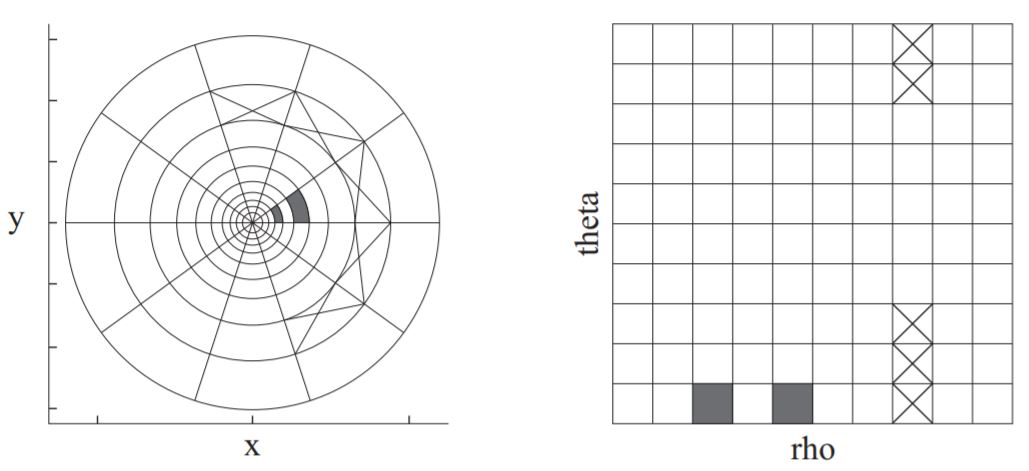
\includegraphics[width=\textwidth]{5/logPol.jpg}
  \caption{Illustration of the relation between Log-Polar and Cartesian coordinates \cite{sarvaiya2012image}}
  \label{fig:sans:logPol} % \label has to be placed AFTER \caption (or \subcaption) to produce correct cross-references.
\end{figure}

\par
The Fourier-Mellin descriptors extracted from the three different sized neighborhoods around the user input represent the noise, after that every pixel of the input sample is examined for correspondence with the metric defined in the first section of this chapter \ref{FMcorr}.
The diameter of the neighborhoods is determined experimentally and is set to 6, 12 and 18 respectively.
The borders of the image are extended by mirroring additionally to ensure that the calculated Fourier-Mellin features have uniform size for every pixel on the image.
The calculated similarities are stored in a correlation map by taking the average correspondence value of the three different sized subimages, and the correlation map is binarized by Otsu's method afterwards.
This thresholding method was used for two reasons, first, it is popular in the forensic image processing for all three kinds of datasets, i.e. at synthetic \cite{algarni2008novel}, \cite{alizadeh2017automatic}, restricted \cite{kong2014novel} and also at real forensic samples \cite{wu2019crime}.
Second, with a global thresholding method the pivot value between fore- and background pixels are found.
To complete the background mask, morphological operations are applied, using an experimentally defined, 8x8 kernel, Opening first and Closing second, to eliminate small holes and rough contours as proposed by many approaches for shoeprint identification \cite{wang2014automatic}, \cite{kong2014novel}, \cite{li2014retrieval}, \cite{tang2010footwear}.
\par
Once the background mask is generated the foreground is processed to suppress the noise and enhance the information.
The mask eliminates the noise in the background area, however, it does not modify the foreground, thus this region is examined.
Noise on the shoeprint pattern is suppressed first, afterwards the edge information is extracted and the binary image is lastly generated.
On the foreground area the noise is located on the shoeprint pattern itself, to preserve the underlying shoeprint information frequency based noise suppression is applied.
Wavelet transform is often used for natural image denoising \cite{xu2016image}, \cite{sugamya2016image}, for fingerprint \cite{li2012texture} and for shoeprint impression enhancement \cite{katireddy2017novel} as well.
During wavelet transform the image is decomposed into subbands, and the subimages are processed separately.
In case of four subbands, the LL image contains the edge information and the other ones the intensity values.
Depending on the properties of the noise the image clutter is separated from the information and suppressed on the corresponding sub-band.
After that the image is reconstructed by inverting the decomposition process.
\par
The same principle is used in this approach but instead of wavelet transform, Fourier transform is applied, to further exploit the previous step of the algorithm.
The Fourier representation of every pixel on the shoeprint sample is calculated using the Discrete Fourier Transform on a 6x6 window, the smallest neighborhood used in the previous step.
This time the window size is fixed, since the final model is based on the neighborhood of every background pixel and not only on the area around the user input.
When the background is separated two models of the appearance of the noise are built, one by averaging the Fourier representations of the background pixels and another by calculating the centroids of the k-means algorithm applied on the background area.
The k-means algorithm is set to terminate after 10 iterations, whereas k equals to 8, so 8 centroids are determined, thus 8 submodels are used when eliminating the noise on the pattern.
These parameters were set experimentally by focusing on the robustness and versatility of the submodels.
Increasing k more submodels are calculated, thus the noise description is more versatile, but in the same time the single submodels, the centroids, are based on a smaller set of pixels, therefore they are more sensitive for outliers as well. 
The noise is suppressed by calculating the difference between the noise model and the Fourier representations of the foreground pixels.
In case of the averaged noise model, the Fourier image of noise is subtracted from the Fourier image of the foreground pixel and its neighborhood and the image is reconstructed using the Inverse Fourier Transform.
When using the centroid noise models, the Fourier image of the foreground pixel is compared to all possible submodels, and the one with highest correlation is used.
The correlation coefficient is determined using the Equation for Fourier-Mellin Feature comparison \ref{FMcorr}.
When the centroid is decided the difference between both Fourier images is calculated and the foreground is reconstructed again using the Inverse Fourier Transform.
The performance and the advantages of both noise representations is discussed in the following chapter.
If the background area is smaller than a given threshold, this step is skipped, because in this case no robust model about the noise can be made.
In this case it is set to 20\% of the image which was determined experimentally.
\par
For line extraction and shoeprint enhancement a gradient based method published by Zeng et al. \cite{zeng2011region} is used.
They propose a region based non-local means algorithm to denoise natural images.
Non-local means was developed for image denoising and grants better smoothing while preserving the details on the image than local mean calculation \cite{buades2005non}.
This is achieved by the averaging pixels with similar properties and not the ones within the same neighborhood.
In non-local means the image is separated into patches which are clustered according to a given criteria.
While smoothing the average value of the patches within the same class is calculated and the members are updated.
Zeng et al. \cite{zeng2011region} propose to use the gradient information of the pixels for classification, which is ideal for shoeprint impressions because the shoeprint pattern is built from a structure of edges.
Since the classification is made based on the gradients, edge properties are the essential clustering criteria.
Assuming that both the shoeprint pattern and the remaining noise on the image have common properties which are different to each other, pattern and noise classes are created at the end of the custering.
In this way the outlines of the shoeprint pattern are preserved and with the non-local menas algorithm the residual noise is smoothed.
\par 
The pixels are clustered according to the eigenvalues of the tensor matrix given by \cite{zeng2011region}:
\[T_\sigma = 
\begin{pmatrix}
t_{11} & t_{12} \\
t_{12} & t_{22}
\end{pmatrix}
=
\begin{pmatrix}
G_\sigma*(g_x(i,j))^2 & G_{\sigma}*g_x(i, j)g_y(i, j)\\
G_{\sigma}*g_y(i, j)g_x(i, j) & G_{\sigma}*(g_y(i, j))^2
\end{pmatrix}
\]

where $g_x$ and $g_y$ represent the gradient information in the corresponding directions and $G_\sigma$ is the Gaussian kernel having $\sigma$ as standard deviation.
To do so, the image is blurred first with the Gaussian kernel of experimentally defined size of 11x11 to make the calculation more robust.
To extract the gradients the Sobel filter is used in x and y direction separately.
The eigenvalues of $T_\sigma$ are then given by \cite{zeng2011region}:
\[\lambda_1 = \frac{1}{2}(t_{11} + t_{22} + \sqrt{(t_{11}-t_{22})^2 + 4t_{12}^2})\]  
\[\lambda_2 = \frac{1}{2}(t_{11} + t_{22} - \sqrt{(t_{11}-t_{22})^2 + 4t_{12}^2})\]  
\label{eig}


The classification is based on the difference between the two eigenvalues of the given pixel.
If the difference is small it indicates smooth region, whereas a higher value implies edge area.
The proposed classification strategy is the following \cite{zeng2011region}:
\[
(i, j)\in \left\{
                \begin{array}{ll}
                  c_1, if \lambda(i,j) \leq \lambda_{min} + \frac{1(\lambda_{max} - \lambda_{min})}{n}\\
                  c_2, if \lambda(i,j) \leq \lambda_{min} + \frac{2(\lambda_{max} - \lambda_{min})}{n}\\
				... \\
                   c_n, if \lambda(i,j) \leq \lambda_{min} + \frac{n(\lambda_{max} - \lambda_{min})}{n}
                \end{array}
              \right.
\]

where $\lambda_{min}$ and $\lambda_{max}$ stays for the minimum and maximum difference on the entire image.
In this thesis two parameter settings are implemented using 25 and 20 classes, which were determined experimentally.
Their comparison and the discussion about their performance is given in the following chapter.
For denoising the mean illumination value of pixels in the same class is calculated and the original pixel value is replaced with the average of the cluster.
Zeng et al. \cite{zeng2011region} propose an additional weighting scheme for mean calculation as well, so that pixels in the same class with smaller geometrical distance have a higher weight than those further away on the image.
However, the weighting method is skipped in this implementation since geometrical location is not relevant in this use-case for two reasons.
First, the size of the region the image was taken of is generally significantly smaller than the scene on natural images.
Second, the shoeprint impressions are 2-Dimensional images in their original form as well. 
Since there is no depth difference within the image, the entire area is considered as one connected region unlike on natural images where the objects in the foreground and the background do not belong together.
But another criteria is added to the clustering algorithm.
After determining the classes based on whether one or more groups have more members than a given threshold, histogram equalization is applied on the image where the differences of eigenvalues are stored, and the classes are recalculated.
This threshold is set to be 60\% experimentally.
This optimization is needed to lower the chance that pattern and noise edges are assigned to the same cluster. 
\par
To find  the cluster with the noise edges a simple heuristic is defined.
Since the clustering algorithm is applied on the entire image, not only on the foreground, the class with the highest amount of members is eliminated.
This decision is based on the assumption that noise is found at the entire image, whereas pattern edges are located only at given areas.
Furthermore, it is also assumed that unlike shoeprint contours, where the edge properties change according to the original shoeprint structures and pressure, noise have similar appearance throughout the the entire sample.
In case of using Histogram Equalization, however, the class memberships are more balanced, so no such heuristic is assumed.
\par
In the next step, the image is binarized with the adaptive thresholding technique \cite{laine1996multiscale} popular in both fields including shoeprint recognition  \cite{wang2014automatic}, \cite{li2014retrieval} and natural image processing \cite{xu2016image}.
Adaptive thresholding is a local binarization technique similar to NBM, generating multiple thresholds for every subregion of an image based on the Gaussian weighted sum in the window, which is experimentally set to 12 in this implementation.
\par
The closing step is postprocessing, where small discontinuities and remaining noise are eliminated.
Despite that in the previous step noise edges belonging to the biggest class were eliminated, other noise lines assigned to different classes are still part of the image.
This problem is solved with short line elimination.
To eliminate noise while preserving the shoe pattern edges the same assumption is made as the one in the previous section.
The noise consists of cluttered small components whereas the shoeprint is built of bigger, connected structures, thus the remaining small regions, smaller than a given threshold, are eliminated from the image.
The connected components of the image using 8-connectivity are extracted and every element with an area not bigger than 15 is deleted immediately.
This threshold is set manually and is significantly smaller than those in the previous section deleting every structure smaller than 50 or open structures smaller than 60 immediately.
This time the majority of noise is already eliminated, since the background is masked, and adaptive thresholding does not generate such high amount of thresholding artifacts and noise clutter than NBM does.
Because only the residual noise around the outlines of the shoeprint has to be deleted, no such high threshold for small structure elimination is set.

%%%%%%%%%%%%%%%%%%%%%%%%%%%%%%%%%%%%%%%%%%%%%%%%%%%%%%%%%%%%%%%%%%%%%%%%%
\chapter{Results and Discussion}
\label{results}
\par
In this chapter the experimental results of the presented algorithms are shown and it is discussed if they are usable for enhancement of real-life footwear impressions from the FID-300 dataset.
Along the qualitative evaluation of all algorithms the quantitative evaluation of the most promising one is also given.
All algorithms are written in Python 2.7 \cite{van1995python} using OpenCV 4.1.1 \cite{opencv_library}.

\section{Qualitative Evaluation}
In this section the qualitative evaluation of the three proposed algorithms is given.
Based on the results, their advantages and disadvantages are examined and possible ways for improvement are discussed.  
\subsection{Feature Learning Algorithm}
\par
Two kinds of experiments were conducted to test the performance of the descriptor, testing on the training set and testing on an evaluation set, on shoeprint impressions which were not considered while training.
The first scenario is discussed now, and the results of the second one afterwards.
Tests are conducted on the training set to see how many descriptors from the original image were eliminated and to identify the common features in the training dataset, Figure \ref{fig:pe:25} and Figure \ref{fig:pe:66} show example results of this testing setup.
The visible difference between Figure \ref{fig:pe:25:LBPs} and Figure \ref{fig:pe:25:LBPb} as well as between Figure \ref{fig:pe:66:LBPs} and Figure \ref{fig:pe:66:LBPb} shows that bigger neighborhood of LBP is a better choice for shoeprint description.
Considering the middle region of Figure \ref{fig:pe:25}, the background on Figure \ref{fig:pe:25:LBPb} is less noisy than on Figure \ref{fig:pe:25:LBPs}.
This difference is more outstanding on  Figure \ref{fig:pe:66} where on Figure \ref{fig:pe:66:LBPs} no shoeprint can be recognized meanwhile on Figure \ref{fig:pe:66:LBPb} outlines of the pattern are visible.
This observation is explained with the properties of the LBP descriptor, a smaller neighborhood is more suitable for detailed, high-frequency textures, however, it is also more sensitive for noise.
A shoeprint impression rather consists of bigger structures and high noise ratio is also common, thus bigger neighborhood is more suitable.
Comparing Figure \ref{fig:pe:25:LBPs} and Figure \ref{fig:pe:66:LBPs} the shoeprint pattern on the first one is better visible, since the original image, Figure \ref{fig:pe:25}, is more clear than Figure \ref{fig:pe:66}.
Still focusing on the middle area of Figure \ref{fig:pe:25}, Figure \ref{fig:pe:25:SIFT} shows that the SIFT descriptor is similarly robust against noise as the LBP descriptor.
SIFT is a robust feature descriptor, thus it is not surprising that it successfully distinguishes between shoeprint and background on a such clear image like Figure \ref{fig:pe:25}.
However, examining Figure  \ref{fig:pe:25:FM} the Fourier-Mellin descriptor has more difficulties with the background area, where the middle regions is less homogen than on  Figure \ref{fig:pe:25:LBPb} and on Figure \ref{fig:pe:25:SIFT}.
On the other hand, inspecting the bottom left side of the shoeprint, it is seen that the Fourier-Mellin features menaged to find the whole area of pattern, whereas only outlines are recognizable on Figure \ref{fig:pe:25:LBPb} and on Figure \ref{fig:pe:25:SIFT}.
That indicates that the Fourier-Mellin features are more detailed descriptors than LBP and SIFT. 
The top part of the shoeprint consist of bigger blobs whereas on the bottom thin lines are seen.
The LBP and SIFT features mistake those lines as noise, because LBP considers a bigger neighborhood and the robustness of the SIFT descriptor prevents to correctly recognize those fine edges.
Fourier-Mellin works on a smaller neighborhood, thus the detailed shoeprint impression parts are more visible, on the other it also causes more noise in the middle of the image.
The same phenomenon is seen on Figures  \ref{fig:pe:66:LBPs} and  \ref{fig:pe:66:LBPb}, where the bottom left regions is clearer on the image  with smaller neighborhood, Figure \ref{fig:pe:66:LBPs}, but the background is more homogeneous on the latter \ref{fig:pe:66:LBPb}. 
That said left bottom region is more recognizable on  \ref{fig:pe:66:LBPs} than on  \ref{fig:pe:66:LBPb}.
Based on these observations,  the features less robust against noise are able to find a higher portion of pattern area than those with higher robustness.
In exchange the background area stays noisy and further image processing is needed.
Comparing all results of the two images, the performance depends on the input quality.
A noisy input, Figure \ref{fig:pe:66}, produces less exact results than a clear sample, Figure \ref{fig:pe:25}.
Feature learning makes it possible to label, thus indicate the shoe pattern area and distinguish it from background, lower quality images as well,  Figure \ref{fig:pe:66}, but in comparison to a higher quality input, Figure \ref{fig:pe:25}, the accuracy is also lower.
That means that the feature learning algorithm does not completely overcome the negative influence of noise, but it makes the descriptors more robust against it.
On Figure \ref{fig:pe:66} and Figure \ref{fig:pe:66:SIFT} the pattern is less recognizable than on the previous example and a higher amount of background pixels are labeled wrongly as pattern.
On noisy images, such as Figure \ref{fig:pe:66} Fourier-Mellin features seem to outperform both SIFT and LBP descriptors.
\par
Overall this testing scenario shows ambivalent results.
On the one hand on clear samples LBP and SIFT is able to distinguish between fore- and background correctly, on the other hand, if the input data is cluttered those two descriptors barely recognize the pattern and the Fourier-Mellin descriptor provides the clearest results.
A solutions for that problem is the combination of the results of the three sources.
Combining all three features possibly leads to a more robust  descriptors, since LBP and SIFT labels the background homogeneously and Fourier-Mellin is more sensitive to shoeprint information.
Another solution is to preprocess the input or use a-priori knowledge about the overall quality, about the visibility of the shoeprint impression, and chose the used descriptors accordingly.

\begin{figure}[h]
  \centering
  \begin{subfigure}[t]{0.19\columnwidth}
    \centering
    \includegraphics[width=\textwidth]{3/00025.jpg}
    \subcaption{}
    \label{fig:pe:25:orig}
  \end{subfigure}
  \begin{subfigure}[t]{0.19\columnwidth}
    \centering
    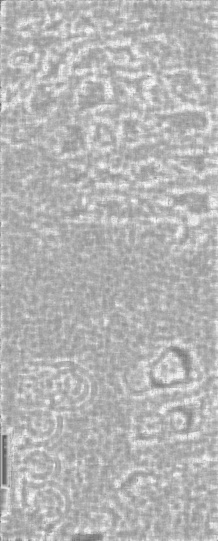
\includegraphics[width=\textwidth]{3/LBP/output_00025.jpg}
    \subcaption{}
    \label{fig:pe:25:LBPs}
  \end{subfigure}
  \begin{subfigure}[t]{0.19\columnwidth}
    \centering
    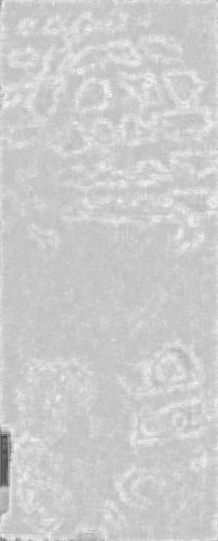
\includegraphics[width=\textwidth]{3/LBP/output_00025_6_24_5.jpg}
    \subcaption{}
    \label{fig:pe:25:LBPb}
  \end{subfigure}
  \begin{subfigure}[t]{0.19\columnwidth}
    \centering
    \includegraphics[width=\textwidth]{3/FM/00025.jpg}
    \subcaption{}
    \label{fig:pe:25:FM}
  \end{subfigure}
  \begin{subfigure}[t]{0.19\columnwidth}
    \centering
    \includegraphics[width=\textwidth]{3/SIFT/00025.jpg}
    \subcaption{}
    \label{fig:pe:25:SIFT}
  \end{subfigure}
  \caption{Output of the feature learning algorithm on an image from training set.\ref{fig:pe:25:orig} Example image from the training set \ref{fig:pe:25:LBPs} Output using LBP descriptors with radius 3 and 12 sample points \ref{fig:pe:25:LBPb} Output using LBP descriptors with radius 5 and 24 sample points \ref{fig:pe:25:FM} Output using Fourier-Mellin Descriptor \ref{fig:pe:25:SIFT} Output using SIFT Descriptor}
  \label{fig:pe:25}
\end{figure}

\begin{figure}[h]
  \centering
  \begin{subfigure}[t]{0.19\columnwidth}
    \centering
    \includegraphics[width=\textwidth]{3/00066.jpg}
    \subcaption{}
    \label{fig:pe:66:orig}
  \end{subfigure}
  \begin{subfigure}[t]{0.19\columnwidth}
    \centering
    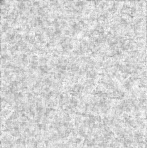
\includegraphics[width=\textwidth]{3/LBP/output_00066_4_12_3.jpg}
    \subcaption{}
    \label{fig:pe:66:LBPs}
  \end{subfigure}
  \begin{subfigure}[t]{0.19\columnwidth}
    \centering
    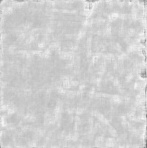
\includegraphics[width=\textwidth]{3/LBP/output_00066_6_24_5.jpg}
    \subcaption{}
    \label{fig:pe:66:LBPb}
  \end{subfigure}
  \begin{subfigure}[t]{0.19\columnwidth}
    \centering
    \includegraphics[width=\textwidth]{3/FM/00066.jpg}
    \subcaption{}
    \label{fig:pe:66:FM}
  \end{subfigure}
  \begin{subfigure}[t]{0.19\columnwidth}
    \centering
    \includegraphics[width=\textwidth]{3/SIFT/00066.jpg}
    \subcaption{}
    \label{fig:pe:66:SIFT}
  \end{subfigure}
  \caption{Output of the feature learning algorithm on an image from training set. \ref{fig:pe:66:orig} Example image from the training set; \ref{fig:pe:66:LBPs} Output using LBP descriptors with radius 3 and 12 sample points; \ref{fig:pe:66:LBPb} Output using LBP descriptors with radius 5 and 24 sample points; \ref{fig:pe:66:FM} Output using Fourier-Mellin Descriptor; \ref{fig:pe:66:SIFT} Output using SIFT Descriptor}
  \label{fig:pe:66}
\end{figure}

\par
In the second testing scenario an evaluation image set is defined, which consist of non-training shoeprint imressions, to examine if the features learned on samples from one shoe are able to describe other shoeprint impressions as well.
On Figure \ref{fig:pe:182} the results of the Feature Learning algorithm on a non-training sample are shown.
The results displayed on Figure \ref{fig:pe:182:LBPs} and on Figure \ref{fig:pe:182:LBPb} strengthens the observation that bigger neighborhood LBP outperforms the smaller radius descriptor.
On Figure \ref{fig:pe:LPBexp} further examples are shown, on Figures \ref{fig:pe:204:LBPb}, \ref{fig:pe:241:LBPb} the original pattern is more visble than on Figures \ref{fig:pe:204:LBPs}, \ref{fig:pe:241:LBPs}, because of the bigger neighborhood settings.
Furthermore examining the middle, noisy part of the images in all three cases a homogenous background is seen containing some falsely labeled pixels.
Observing the bottom part of the shoe a weakness of LBP and SIFT already discussed is noticeable.
On the original image there are small structures in the bottom area which are part of the shoeprint.
Similarly as on the bottom left part of Figure \ref{fig:pe:25} the fine structures are partially recognized, comparing Figure \ref{fig:pe:182:FM} to Figure \ref{fig:pe:182:LBPb} and to Figure \ref{fig:pe:182:SIFT} Fourier-Mellin outperforms LBP and SIFT again labeling the whole area and not only the outlines correctly.
This results indicate similar behavior like discussed above, that means that the feature pool assembled based on samples of one shoe are suitable for impressions of other shoeprints as well.
But it also suffers from the same limitations which is possibly solved with the two approaches discussed above, namely with the combined use of all three descriptors or taking advantage on a-priori knowledge or applying a preprocessing algorithm to determine the input quality and use one descriptor accordingly.

\begin{figure}[h]
  \centering
  \begin{subfigure}[t]{0.19\columnwidth}
    \centering
    \includegraphics[width=\textwidth]{3/00182.jpg}
    \subcaption{}
    \label{fig:pe:182:orig}
  \end{subfigure}
  \begin{subfigure}[t]{0.19\columnwidth}
    \centering
    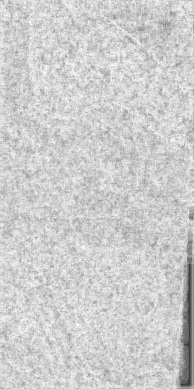
\includegraphics[width=\textwidth]{3/LBP/output_00182_4_12_3.jpg}
    \subcaption{}
    \label{fig:pe:182:LBPs}
  \end{subfigure}
  \begin{subfigure}[t]{0.19\columnwidth}
    \centering
    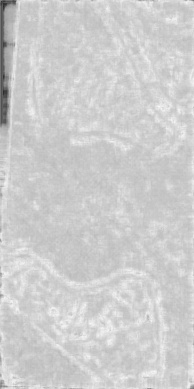
\includegraphics[width=\textwidth]{3/LBP/output_00182_6_24_5.jpg}
    \subcaption{}
    \label{fig:pe:182:LBPb}
  \end{subfigure}
  \begin{subfigure}[t]{0.19\columnwidth}
    \centering
    \includegraphics[width=\textwidth]{3/FM/00182.jpg}
    \subcaption{}
    \label{fig:pe:182:FM}
  \end{subfigure}
  \begin{subfigure}[t]{0.19\columnwidth}
    \centering
    \includegraphics[width=\textwidth]{3/SIFT/00182.jpg}
    \subcaption{}
    \label{fig:pe:182:SIFT}
  \end{subfigure}
  \caption{Output of the feature learning algorithm \ref{fig:pe:182:orig} Input image; \ref{fig:pe:182:LBPs} Output using LBP descriptors with radius 3 and 12 sample points; \ref{fig:pe:182:LBPb} Output using LBP descriptors with radius 5 and 24 sample points; \ref{fig:pe:182:FM} Output using Fourier-Mellin Descriptor; \ref{fig:pe:182:SIFT} Output using SIFT Descriptor}
  \label{fig:pe:182}
\end{figure}

\begin{figure}[h]
  \centering
	\begin{subfigure}[t]{0.16\columnwidth}
    \centering
    \includegraphics[width=\textwidth]{5/1/00204.jpg}
    \subcaption{}
    \label{fig:pe:204:orig}
  \end{subfigure}
  \begin{subfigure}[t]{0.16\columnwidth}
    \centering
    \includegraphics[width=\textwidth]{5/1/output_00204_4_12_3.jpg}
    \subcaption{}
    \label{fig:pe:204:LBPs}
  \end{subfigure}
  \begin{subfigure}[t]{0.16\columnwidth}
    \centering
    \includegraphics[width=\textwidth]{5/1/output_00204_6_24_5.jpg}
    \subcaption{}
    \label{fig:pe:204:LBPb}
  \end{subfigure}
  \begin{subfigure}[t]{0.16\columnwidth}
    \centering
    \includegraphics[width=\textwidth]{5/1/00241.jpg}
    \subcaption{}
    \label{fig:pe:241:orig}
  \end{subfigure}
  \begin{subfigure}[t]{0.16\columnwidth}
    \centering
    \includegraphics[width=\textwidth]{5/1/output_00241_4_12_3.jpg}
    \subcaption{}
    \label{fig:pe:241:LBPs}
  \end{subfigure}
  \begin{subfigure}[t]{0.16\columnwidth}
    \centering
    \includegraphics[width=\textwidth]{5/1/output_00241_6_24_5.jpg}
    \subcaption{}
    \label{fig:pe:241:LBPb}
  \end{subfigure}
  \caption{\ref{fig:pe:204:orig}, \ref{fig:pe:241:orig} Original shoeprint impressions; \ref{fig:pe:204:LBPs}, \ref{fig:pe:241:LBPs} Output using LBP descriptors with radius 3 and 12 sample points; \ref{fig:pe:204:LBPb}, \ref{fig:pe:241:LBPb} Output using LBP descriptors with radius 5 and 24 sample points}
  \label{fig:pe:LPBexp}
\end{figure}

\par
To summarize LBP and SIFT features are less responsive in the noisy area and have difficulties to find fine patterns while the Fourier-Mellin transform labels bigger parts of the shoeprint correctly whereas it more often mistakes the noise as foreground.
Based on the testing images Fourier-Mellin recognize the shoeprint pixels in noisy images better than LBP and SIFT.
A possible solution is to combine all three feature descriptors and propose a weighting score across them, assuming that all three feature sets were able to provide usable results for further processing.
There are multiple ways to distribute the weights, for example using a-priori knowledge or user input or to measure the quality of the output and set the weights accordingly.
A quality measurement technique is to invent a heuristic about the area of the shoeprint, for example it is between 20\% and 40\% of the entire image, and to calculate that on the labeled image as well.
If the output of one descriptor fulfills the heuristic its weight increases, and the weight is decreased in every other case.
\par
There are lower quality samples in the dataset available then the one presented on Figure  \ref{fig:pe:66} where there is small contrast between the pattern and the background, Figure  \ref{fig:int:cap:neg}, or there is a high amount of noise on the fore- and the background as well, Figure \ref{fig:rw:lowFID}.
The feature pool is created based on a limited training set of seven images.
Incorporating more samples and altering the learning criteria, e.g. the given feature has to be found in a given ratio of training images and not on every one of them, leads to a broader feature pool containing a higher amount of descriptors, which are descriptive for a possible wider range of shoeprint impressions as well.
However, this also increases the chance of selecting more noise descriptors into the final feature set.

\subsection{Fully-Automated Noise Elimination Algorithm}
\par
Figures \ref{fig:fans:denoise} and \ref{fig:fans:enhance} show the output of the proposed algorithm on every stage and present the final results as well.
The former one shows the output of the denoising step on three example images from the FID-300 database.
In the second column the Wiener filtered images are shown, in the third one the Bilateral filtered images are displayed whereas the combination of those two pictures is in the last column.
Considering the background of the algorithms and the amount of noise on the images, a light smoothing is done during the denoising phase.
This decision was made to protect the valuable pattern information.
Since no previous knowledge is available about the properties of shoe print, no aggressive filter kernel, the  size of both kernels is small being only 5x5, is used to make sure that the relevant information is preserved.
On the combined image, the contrast between fore- and background is increased.
Since both filters smooth the background area and preserve the shoeprint, their combination amplifies the blurring effect without damaging the pattern information. 
Despite the amplifying effect, bigger noise elements, such as the white clutter on Figure \ref{fig:fans:235:orig}, are not eliminated, because of the weak smoothing.  
Chatterjee et al. \cite{chatterjee2011patch} proposed a method which represents the estimated image for Wiener Filter based on geometrically and photometrically similar regions, so that strong blurring is possible without damaging the foreground area.
Even though their approach had promising results, it was tested on data with Gaussian noise, similar to Figure \ref{fig:fans:241:orig}, and not with irregular cluttered noise seen on the majority of FID-300 images, for example on Figure \ref{fig:fans:235:orig} and on the top of Figure \ref{fig:fans:21:orig}.
\par
The second step of the algorithm is enhancement, where SMQT is applied, and the results are shown on Figures \ref{fig:fans:241:enhance}, \ref{fig:fans:235:enhance} and \ref{fig:fans:21:enhance}.
The benefits of the SMQT algorithm are ambiguous.
On the one hand, focusing on the middle area of Figures  \ref{fig:fans:241:enhance} and \ref{fig:fans:235:enhance} the difference between fore- and background is bigger than on the original image.
The contours of the shoeprint are more outstanding than on the original image.
Comparing Figure \ref{fig:fans:235:enhance} to Figure \ref{fig:fans:21:denoise}, the shoe pattern structures got darker and there is a brighter area around the contours than on Figure \ref{fig:fans:21:denoise}.
On the other hand, not only the information but also the remaining noise elements became enhanced by SMQT.
Even though the denoising stage is finished, since only moderate smoothing was applied, there is a considerable amount of noise on the input images for SMQT.
The soft filtering is able to cope with Gaussian noise, such as on Figure \ref{fig:fans:241:denoise}, but it does not eliminate bigger clutter particles like on the left side of Figure \ref{fig:fans:235:denoise} or on the upper region of Figure \ref{fig:fans:21:denoise}.
The SMQT enhancement makes these clutter more prominent by increasing the color difference between the noise and the homogeneous background.
For example the already mentioned patches on the left side of Figure \ref{fig:fans:235:denoise} are now more visible than on the original image \ref{fig:fans:235:orig}.
Additionally, SMQT has similar effects to the Histogram Equalization: the background on Figure \ref{fig:fans:241:denoise} is near homogeneous, but after applying SMQT, its color changes are more obvious since the original pixel values are mapped now to a wider color range.
Despite its enhancing effect in the background, SMQT also increases the contrast between the outlines of the shoeprint and its surroundings which is a beneficial feature for the following, local binarization step.

\afterpage{
\begin{figure}[H]

\subfloat{
  \centering
  \begin{subfigure}[t]{0.24\columnwidth}
    \centering
    \includegraphics[width=\textwidth]{4/241/00241.jpg}
    \subcaption{}
    \label{fig:fans:241:orig}
  \end{subfigure}
  \begin{subfigure}[t]{0.24\columnwidth}
    \centering
    \includegraphics[width=\textwidth]{4/241/00241_wiener.jpg}
    \subcaption{}
    \label{fig:fans:241:wiener}
  \end{subfigure}
  \begin{subfigure}[t]{0.24\columnwidth}
    \centering
    \includegraphics[width=\textwidth]{4/241/00241_bi5.jpg}
    \subcaption{}
    \label{fig:fans:241:bi}
  \end{subfigure}
  \begin{subfigure}[t]{0.24\columnwidth}
    \centering
    \includegraphics[width=\textwidth]{4/241/00241_denoise.jpg}
    \subcaption{}
    \label{fig:fans:241:denoise}
  \end{subfigure}
  \caption{}
}

\subfloat{
    \centering
  \begin{subfigure}[t]{0.24\columnwidth}
    \centering
    \includegraphics[width=\textwidth]{4/235/00235.jpg}
    \subcaption{}
    \label{fig:fans:235:orig}
  \end{subfigure}
  \begin{subfigure}[t]{0.24\columnwidth}
    \centering
    \includegraphics[width=\textwidth]{4/235/00235_wiener.jpg}
    \subcaption{}
    \label{fig:fans:235:wiener}
  \end{subfigure}
  \begin{subfigure}[t]{0.24\columnwidth}
    \centering
    \includegraphics[width=\textwidth]{4/235/00235_bi5.jpg}
    \subcaption{}
    \label{fig:fans:235:bi}
  \end{subfigure}
  \begin{subfigure}[t]{0.24\columnwidth}
    \centering
    \includegraphics[width=\textwidth]{4/235/00235_denoise.jpg}
    \subcaption{}
    \label{fig:fans:235:denoise}
  \end{subfigure}
  \caption{}
}

\subfloat{
  \centering
  \begin{subfigure}[t]{0.24\columnwidth}
    \centering
    \includegraphics[width=\textwidth]{4/21/00021.jpg}
    \subcaption{Example image}
    \label{fig:fans:21:orig}
  \end{subfigure}
  \begin{subfigure}[t]{0.24\columnwidth}
    \centering
    \includegraphics[width=\textwidth]{4/21/00021_wiener.jpg}
    \subcaption{Wiener filtered image}
    \label{fig:fans:21:wiener}
  \end{subfigure}
  \begin{subfigure}[t]{0.24\columnwidth}
    \centering
    \includegraphics[width=\textwidth]{4/21/00021_bi5.jpg}
    \subcaption{Bilateral filtered image}
    \label{fig:fans:21:bi}
  \end{subfigure}
  \begin{subfigure}[t]{0.24\columnwidth}
    \centering
    \includegraphics[width=\textwidth]{4/21/00021_denoise.jpg}
    \subcaption{Denoised image}
    \label{fig:fans:21:denoise}
  \end{subfigure}
  \caption{}
}

\caption{Example for the results of the denoising stage
				\ref{fig:fans:241:orig}, \ref{fig:fans:235:orig}, \ref{fig:fans:21:orig} Example image; \ref{fig:fans:241:wiener}, \ref{fig:fans:235:wiener}, \ref{fig:fans:21:wiener} Wiener filtered image; \ref{fig:fans:241:bi}, \ref{fig:fans:235:bi}, \ref{fig:fans:21:bi} Bilateral filtered image; \ref{fig:fans:241:denoise}, \ref{fig:fans:235:denoise}, \ref{fig:fans:21:denoise} Denoised image}
\label{fig:fans:denoise}

\end{figure}
}

\afterpage{
\begin{figure}[H]

\subfloat{
  \centering
  \begin{subfigure}[t]{0.24\columnwidth}
    \centering
    \includegraphics[width=\textwidth]{4/241/00241.jpg}
    \subcaption{}
	\label{fig:fans:241:o}
  \end{subfigure}
  \begin{subfigure}[t]{0.24\columnwidth}
    \centering
    \includegraphics[width=\textwidth]{4/241/00241_enhnace.jpg}
    \subcaption{}
    \label{fig:fans:241:enhance}
  \end{subfigure}
 \begin{subfigure}[t]{0.24\columnwidth}
    \centering
    \includegraphics[width=\textwidth]{4/241/00241_threshold.jpg}
    \subcaption{}
    \label{fig:fans:241:bin}
  \end{subfigure}
  \begin{subfigure}[t]{0.24\columnwidth}
    \centering
    \includegraphics[width=\textwidth]{4/241/00241_result.jpg}
    \subcaption{}
    \label{fig:fans:241:out}
  \end{subfigure}
  \caption{}
}

\subfloat{
    \centering
  \begin{subfigure}[t]{0.24\columnwidth}
    \centering
    \includegraphics[width=\textwidth]{4/235/00235.jpg}
    \subcaption{}
	\label{fig:fans:235:o}
  \end{subfigure}
  \begin{subfigure}[t]{0.24\columnwidth}
    \centering
    \includegraphics[width=\textwidth]{4/235/00235_enhnace.jpg}
    \subcaption{}
    \label{fig:fans:235:enhance}
  \end{subfigure}
 \begin{subfigure}[t]{0.24\columnwidth}
    \centering
    \includegraphics[width=\textwidth]{4/235/00235_threshold.jpg}
    \subcaption{}
    \label{fig:fans:235:bin}
  \end{subfigure}
  \begin{subfigure}[t]{0.24\columnwidth}
    \centering
    \includegraphics[width=\textwidth]{4/235/00235_result.jpg}
    \subcaption{}
    \label{fig:fans:235:out}
  \end{subfigure}
  \caption{}
}

\subfloat{
  \centering
  \begin{subfigure}[t]{0.24\columnwidth}
    \centering
    \includegraphics[width=\textwidth]{4/21/00021.jpg}
    \subcaption{Example image}
	\label{fig:fans:21:o}
  \end{subfigure}
  \begin{subfigure}[t]{0.24\columnwidth}
    \centering
    \includegraphics[width=\textwidth]{4/21/00021_enhnace.jpg}
    \subcaption{}
    \label{fig:fans:21:enhance}
  \end{subfigure}
 \begin{subfigure}[t]{0.24\columnwidth}
    \centering
    \includegraphics[width=\textwidth]{4/21/00021_threshold.jpg}
    \subcaption{}
    \label{fig:fans:21:bin}
  \end{subfigure}
  \begin{subfigure}[t]{0.24\columnwidth}
    \centering
    \includegraphics[width=\textwidth]{4/21/00021_result.jpg}
    \subcaption{}
    \label{fig:fans:21:out}
  \end{subfigure}
  \caption{}
}

\caption{Example for the results of the enhancement and postprocessing stage
				\ref{fig:fans:241:o}, \ref{fig:fans:235:o}, \ref{fig:fans:21:o} Example image; \ref{fig:fans:241:enhance}, \ref{fig:fans:235:enhance}, \ref{fig:fans:21:enhance} Enhanced image; \ref{fig:fans:241:bin}, \ref{fig:fans:235:bin}, \ref{fig:fans:21:bin} Binarized image ; \ref{fig:fans:241:out}, \ref{fig:fans:235:out}, \ref{fig:fans:21:out} Output image}
\label{fig:fans:enhance}

\end{figure}
}
\par
The closing step of the algorithm is postprocessing, consisting of binarization (the third column of Figure \ref{fig:fans:enhance}) and line-clutter elimination (in the fourth column of Figure \ref{fig:fans:enhance}).
As expected NBM, being a local edge sensitive thresholding algorithm, takes advantage of the contrast difference between the outlines of the shoeprint impression and its neighborhood and finds the silhouettes of pattern. 
On all three images, Figure \ref{fig:fans:241:bin}, Figure \ref{fig:fans:235:bin} and Figure \ref{fig:fans:21:out}, the contours of the patterns are visible.
However, the drawbacks of NBM discussed in the previous chapter and the enhanced noise by SMQT are evident, since among the correct outlines a high amount of noise is generated.
In the background and between the space of the shoeprint outlines additional small structures are visible.
For this reason, the closing step of small and open structure elimination is executed.
On Figures \ref{fig:fans:241:out} and \ref{fig:fans:235:out} the majority of background is cleared up and the shoeprint pattern is shown clearly.
On the other hand, on Figure \ref{fig:fans:21:out} the original pattern is not recognizable anymore, as along with the background noise relevant contour edges were also eliminated, and noise lines attached to the shoeprint pattern were kept.
\par
The presented results indicate two things.
First, NBM with the current postprocessing technique works better on samples with fine lines, Figure \ref{fig:fans:241:orig}, and with detailed small structures, Figure \ref{fig:fans:235:orig} than on shoeprint impression consisting bigger geometrical elements, Figure \ref{fig:fans:21:orig}.
As already discussed and shown, NBM tends to generate line noise on homogenous areas, if the shoeprint consist of dense pattern, there is no big, homogenous background between the different structure elements, thus no noise is generated.
To solve this problem, Saxena et al. \cite{saxena2019niblack} analyze several improvements for NBM to make it more robust and performant in such conditions and on lower quality data.
Second, the heuristics which the two postprocessing steps are based on do not apply to every sample of the database.
On Figure  \ref{fig:fans:21:bin} even though there is a high amount of noise, the pattern is clearly recognizable, whereas on Figure \ref{fig:fans:21:out} no shoeprint is seen anymore.
This implies that the settings of the structure elimination algorithms are not detailed enough and that more sophisticated postprocessing is needed, which covers more samples of the database.
Several pattern edges were eliminated because they were too short.
The threshold for line length were not changed during testing, thus a possible solution for the problem is to always adjust the parameter according to the current image.
This adjustment is however difficult, since there is no a-priori knowledge about the given sample available.
Alternatively, looking at Figure  \ref{fig:fans:21:out}, the outlines of the pattern were found originally, but because of the noise they were not connected.
In the application only 8-neighborhood is considered, a more allowing connectivity criteria, such as neighborhood in a given range, leads to closed contour edges.
But this causes more connectivity among noise as well.
Furthermore, it also magnifies the second problem occurring on Figure \ref{fig:fans:21:out}, that noise lines are connected to the contours, thus are not eliminated.
In conclusion, an additional postprocessing step is needed to examine the remaining edges and determine which connection was made unintentionally.
\par
Based on the experiments presented in this section two factors highly influence the output of the algorithm.
These are image quality, such as the appearance of noise and contrast between fore- and background, and the properties of the shoeprint impression, e.g. the density and size of the unit pattern structure.
In conclusion, this algorithm is specialized in a given type of shoeprint impressions in its current form, namely the ones with dense patterns or fine-lined structures. 
In such cases, despite cluttered noise, Figure \ref{fig:fans:235:o}, promising results were generated.
To expand the usability of this algorithm for other samples of FID-300 further improvements, such as detailed noise model for Wiener Filter and variable settings for the postprocessing heuristics, are needed. 

\subsection{Shoeprint Enhancement with Non-Local Means}
\par
In this section the experimental results of the Shoeprint Enhancement Algorithm with Non-Local Means are presented and the performance is discussed.
On Figures \ref{fig:sans:res1} and \ref{fig:sans:res2} example results are shown, the original samples are in the first column, the results using 20 classes for gradient clustering are shown in the second and third column, the output using 25 classes are in the fourth and fifth column.
Column two and four illustrate the results when the average noise model was used for pattern enhancement, whereas column three and five represent the output in case of using the centroids of the k-means algorithm.

\afterpage{
\begin{figure}[H]

\subfloat{
  \centering
  \begin{subfigure}[t]{0.19\columnwidth}
    \centering
    \includegraphics[width=\textwidth]{5/21/orig.jpg}
    \subcaption{}
	\label{fig:sans:21}
  \end{subfigure}
  \begin{subfigure}[t]{0.19\columnwidth}
    \centering
    \includegraphics[width=\textwidth]{5/21/20_mean.jpg}
    \subcaption{}
    \label{fig:sans:21:20_mean}
  \end{subfigure}
  \begin{subfigure}[t]{0.19\columnwidth}
    \centering
    \includegraphics[width=\textwidth]{5/21/20_cent.jpg}
    \subcaption{}
    \label{fig:sans:21:20_cent}
  \end{subfigure}
  \begin{subfigure}[t]{0.19\columnwidth}
    \centering
    \includegraphics[width=\textwidth]{5/21/25_mean.jpg}
    \subcaption{}
    \label{fig:sans:21:25_mean}
  \end{subfigure}
  \begin{subfigure}[t]{0.19\columnwidth}
    \centering
    \includegraphics[width=\textwidth]{5/21/25_cent.jpg}
    \subcaption{}
    \label{fig:sans:21:25_cent}
  \end{subfigure}
  \caption{}
}

\subfloat{
  \centering
  \begin{subfigure}[t]{0.19\columnwidth}
    \centering
    \includegraphics[width=\textwidth]{5/25/orig.jpg}
    \subcaption{}
	\label{fig:sans:25}
  \end{subfigure}
  \begin{subfigure}[t]{0.19\columnwidth}
    \centering
    \includegraphics[width=\textwidth]{5/25/20_mean.jpg}
    \subcaption{}
    \label{fig:sans:25:20_mean}
  \end{subfigure}
  \begin{subfigure}[t]{0.19\columnwidth}
    \centering
    \includegraphics[width=\textwidth]{5/25/20_cent.jpg}
    \subcaption{}
    \label{fig:sans:25:20_cent}
  \end{subfigure}
  \begin{subfigure}[t]{0.19\columnwidth}
    \centering
    \includegraphics[width=\textwidth]{5/25/25_mean.jpg}
    \subcaption{}
    \label{fig:sans:25:25_mean}
  \end{subfigure}
  \begin{subfigure}[t]{0.19\columnwidth}
    \centering
    \includegraphics[width=\textwidth]{5/25/25_cent.jpg}
    \subcaption{}
    \label{fig:sans:25:25_cent}
  \end{subfigure}
  \caption{}
}

\caption{Example results of the Shoeprint Enhancement algorithm
				\ref{fig:sans:21}, \ref{fig:sans:25} Example image; \ref{fig:sans:21:20_mean}, \ref{fig:sans:25:20_mean} Enhanced image using average noise model and 20 clusters for gradient classification; \ref{fig:sans:21:20_cent}, \ref{fig:sans:25:20_cent} Enhanced image using centroids noise model and 20 clusters for gradient classification; \ref{fig:sans:21:25_mean}, \ref{fig:sans:25:25_mean} Enhanced image using average noise model and 25 clusters for gradient classification; \ref{fig:sans:21:25_cent}, \ref{fig:sans:25:25_cent} Enhanced image using average noise model and 25 clusters for gradient classification}
\label{fig:sans:res1}

\end{figure}
}


\par
The example images,  \ref{fig:sans:res1} and \ref{fig:sans:res2}, show that varying the algorithm parameters makes a significant difference when the input had low quality.
This is explained with two factors.
First, high quality images have less noise on the pattern, Figures \ref{fig:sans:21} and \ref{fig:sans:204}, or the noise is less varying, Figure \ref{fig:sans:21}, than on a lower quality sample, Figure \ref{fig:sans:174}.
Second, using 20 and 25 classes for the non-local means algorithm is overstated, on high quality images there is no high variance between the properties of edges thus classes with little amount of members are generated .
However choosing high amount of classes was an intentional decision, first, the structure of the image is better preserved, when the means are calculated on a high amount of subgroups, second, using fewer classes leads to eliminating valuable pattern information when deleting the members of the most populated class.
Comparing the output of the two different kinds of noise models, there is little difference between their performance.
Both models were able to preserve the pattern information where the foreground is not cluttered like on Figure \ref{fig:sans:25}.
Focusing on small details like the top of Figure \ref{fig:sans:21} the average noise model is more aggressive than the centroid one.
That observation corresponds to the calculation of the noise representation, taking the average of every noise pixel results in a less detailed model than calculating more representatives, thus it is more destructive than the centroid representation.
On the result images of Figure \ref{fig:sans:204} significant shoeprint pattern parts are missing on the bottom area.
That is the combined effect of those steps where the heuristic is assumed, that small regions represent noise elements rather than relevant pattern information.
Therefore the fine-lines of the shoeprint pattern are wrongly considered as noise and are eliminated.

\par
On Figure \ref{fig:sans:pip} the entire pipeline of the Shoeprint Enhancement algorithm is shown on two example images.
On Figures  \ref{fig:sans:pip:21:bg} \ref{fig:sans:pip:204:bg} and \ref{fig:sans:pip:239:bg} the binary mask is shown, where white denotes the background and black the foreground area.
Inspecting the images the majority of the background is labeled correctly, however two limitations are visible.
The first one is the bottom area of Figure \ref{fig:sans:pip:204:bg}, where half of the fine-lined area of the actual shoeprint is cropped.
The noise model is not able to distinguish between the structured noise in the background and the detailed shoeprint pattern in the foreground.
Furthermore, the fine-lines cover a small area of the three different sized neighborhoods when calculating the correlation with the noise model, therefore high similarity is noted.
In this context the fine-lines of the shoeprint pattern are considered as "noise" when comparing the model about the background, namely the noise model, and the neighborhood of that given area.
And, because of the robustness of the Fourier-Mellin features, the thin lines of the shoeprint impression have little influence, thus that area is falsely labeled.
The other one is on Figures \ref{fig:sans:pip:21:bg} and \ref{fig:sans:pip:239:bg}, where, because of the significant change within the background, the border area is labeled as foreground.

\afterpage{
\begin{figure}[H]

\subfloat{
  \centering
  \begin{subfigure}[t]{0.19\columnwidth}
    \centering
    \includegraphics[width=\textwidth]{5/174/orig.jpg}
    \subcaption{}
	\label{fig:sans:174}
  \end{subfigure}
  \begin{subfigure}[t]{0.19\columnwidth}
    \centering
    \includegraphics[width=\textwidth]{5/174/20_mean.jpg}
    \subcaption{}
    \label{fig:sans:174:20_mean}
  \end{subfigure}
  \begin{subfigure}[t]{0.19\columnwidth}
    \centering
    \includegraphics[width=\textwidth]{5/174/20_cent.jpg}
    \subcaption{}
    \label{fig:sans:174:20_cent}
  \end{subfigure}
  \begin{subfigure}[t]{0.19\columnwidth}
    \centering
    \includegraphics[width=\textwidth]{5/174/25_mean.jpg}
    \subcaption{}
    \label{fig:sans:174:25_mean}
  \end{subfigure}
  \begin{subfigure}[t]{0.19\columnwidth}
    \centering
    \includegraphics[width=\textwidth]{5/174/25_cent.jpg}
    \subcaption{}
    \label{fig:sans:174:25_cent}
  \end{subfigure}
  \caption{}
}


\subfloat{
  \centering
  \begin{subfigure}[t]{0.19\columnwidth}
    \centering
    \includegraphics[width=\textwidth]{5/204/orig.jpg}
    \subcaption{}
	\label{fig:sans:204}
  \end{subfigure}
  \begin{subfigure}[t]{0.19\columnwidth}
    \centering
    \includegraphics[width=\textwidth]{5/204/20_mean.jpg}
    \subcaption{}
    \label{fig:sans:204:20_mean}
  \end{subfigure}
  \begin{subfigure}[t]{0.19\columnwidth}
    \centering
    \includegraphics[width=\textwidth]{5/204/20_cent.jpg}
    \subcaption{}
    \label{fig:sans:204:20_cent}
  \end{subfigure}
  \begin{subfigure}[t]{0.19\columnwidth}
    \centering
    \includegraphics[width=\textwidth]{5/204/25_mean.jpg}
    \subcaption{}
    \label{fig:sans:204:25_mean}
  \end{subfigure}
  \begin{subfigure}[t]{0.19\columnwidth}
    \centering
    \includegraphics[width=\textwidth]{5/204/25_cent.jpg}
    \subcaption{}
    \label{fig:sans:204:25_cent}
  \end{subfigure}
  \caption{}
}

\caption{Example results of the Shoeprint Enhancement algorithm
				\ref{fig:sans:174}, \ref{fig:sans:204} Example image; \ref{fig:sans:174:20_mean}, \ref{fig:sans:204:20_mean} Enhanced image using average noise model and 20 clusters for gradient classification; \ref{fig:sans:174:20_cent}, \ref{fig:sans:204:20_cent} Enhanced image using centroids noise model and 20 clusters for gradient classification; \ref{fig:sans:174:25_mean}, \ref{fig:sans:204:25_mean} Enhanced image using average noise model and 25 clusters for gradient classification; \ref{fig:sans:174:25_cent}, \ref{fig:sans:204:25_cent} Enhanced image using average noise model and 25 clusters for gradient classification}
\label{fig:sans:res2}

\end{figure}
}

\par
The appearance of the input image after eliminating the noise in the foreground is shown in the third column.
Figures  \ref{fig:sans:pip:204:bg} and \ref{fig:sans:pip:239:bg} illustrate that the noise suppression technique does not damage the pattern area, the difference between the fore- and the background is preserved.
On Figure \ref{fig:sans:pip:21} there is significant noise on the top region of the foreground, which is successfully suppressed on Figure \ref{fig:sans:pip:21:enh}.
This indicates that, as expected, the noise and the shoeprint impression itself have different Fourier representations.
Working in the Fourier domain, the noise frequencies are eliminated and the pattern is successfully reconstructed.
\par
Focusing on the background of the images in the fourth column, nearly homogeneous background is created without applying the noise mask on the images.
However, on Figure \ref{fig:sans:pip:204:grad} a weakness of the algorithm is also visible.
The non-local mean calculation eliminates the majority of pattern information in both top and bottom area of the original shoeprint.
Combined with structured background noise, several mixed classes are generated where noise and pattern data occur simultaneously.
The artifacts of this phenomenon are visible not only on the said shoeprint pattern area, but also in the middle of the image, where noise structures were enhanced appearing as bright lines similar to the remaining pattern edges.
\par
Figures \ref{fig:sans:pip:21:th}, \ref{fig:sans:pip:204:th} and \ref{fig:sans:pip:239:th} show the binarized images after applying the background mask.
Because of the nearly homogeneous background achieved by non-local means, the thresholding method is able to preserve the extracted lines.
With the masking, the falsely clustered edges from the previous step, such as the ones in the middle of Figure \ref{fig:sans:pip:204:grad}, are deleted.
\par
In the last column the final results are shown after the postprocessing step of eliminating small regions.
Comparing Figure \ref{fig:sans:pip:21:th} to  Figure \ref{fig:sans:pip:21:res} the latter is less cluttered, there is less noise in the background, small lines around the pattern contours are eliminated successfully while no relevant edges, the outlines of the shoeprint, were deleted.
The same effect is also visible on Figure \ref{fig:sans:pip:239:res}, where the silhouette of the pattern is clearer since the majority of remaining line noise was eliminated.
However, on Figure \ref{fig:sans:pip:204:res} the pattern information is further damaged by the postprocessing step.
Observing the right side of the bottom area it is visible that several pattern contours were eliminated.
The postprocessing step assumes that the shoeprint consists of bigger structures such as filled geometries on Figure \ref{fig:sans:pip:21} or broad edges on Figure \ref{fig:sans:pip:239}, thus the fine-lined edge pattern of Figure \ref{fig:sans:pip:204} is automatically considered as noise instead of relevant information.


\afterpage{
\begin{figure}[H]

\subfloat{
  \centering
  \begin{subfigure}[t]{0.16\columnwidth}
    \centering
    \includegraphics[width=\textwidth]{5/pipeline/21/orig.jpg}
    \subcaption{}
	\label{fig:sans:pip:21}
  \end{subfigure}
  \begin{subfigure}[t]{0.16\columnwidth}
    \centering
    \includegraphics[width=\textwidth]{5/pipeline/21/mask.jpg}
    \subcaption{}
    \label{fig:sans:pip:21:bg}
  \end{subfigure}
  \begin{subfigure}[t]{0.16\columnwidth}
    \centering
    \includegraphics[width=\textwidth]{5/pipeline/21/enhance.jpg}
    \subcaption{}
    \label{fig:sans:pip:21:enh}
  \end{subfigure}
  \begin{subfigure}[t]{0.16\columnwidth}
    \centering
    \includegraphics[width=\textwidth]{5/pipeline/21/grad.jpg}
    \subcaption{}
    \label{fig:sans:pip:21:grad}
  \end{subfigure}
  \begin{subfigure}[t]{0.16\columnwidth}
    \centering
    \includegraphics[width=\textwidth]{5/pipeline/21/th.jpg}
    \subcaption{}
    \label{fig:sans:pip:21:th}
  \end{subfigure}
  \begin{subfigure}[t]{0.16\columnwidth}
    \centering
    \includegraphics[width=\textwidth]{5/pipeline/21/res.jpg}
    \subcaption{}
    \label{fig:sans:pip:21:res}
  \end{subfigure}
  \caption{}
}

\subfloat{
  \centering
  \begin{subfigure}[t]{0.16\columnwidth}
    \centering
    \includegraphics[width=\textwidth]{5/pipeline/204/orig.jpg}
    \subcaption{}
	\label{fig:sans:pip:204}
  \end{subfigure}
  \begin{subfigure}[t]{0.16\columnwidth}
    \centering
    \includegraphics[width=\textwidth]{5/pipeline/204/mask.jpg}
    \subcaption{}
    \label{fig:sans:pip:204:bg}
  \end{subfigure}
  \begin{subfigure}[t]{0.16\columnwidth}
    \centering
    \includegraphics[width=\textwidth]{5/pipeline/204/enhance.jpg}
    \subcaption{}
    \label{fig:sans:pip:204:enh}
  \end{subfigure}
  \begin{subfigure}[t]{0.16\columnwidth}
    \centering
    \includegraphics[width=\textwidth]{5/pipeline/204/grad.jpg}
    \subcaption{}
    \label{fig:sans:pip:204:grad}
  \end{subfigure}
  \begin{subfigure}[t]{0.16\columnwidth}
    \centering
    \includegraphics[width=\textwidth]{5/pipeline/204/th.jpg}
    \subcaption{}
    \label{fig:sans:pip:204:th}
  \end{subfigure}
  \begin{subfigure}[t]{0.16\columnwidth}
    \centering
    \includegraphics[width=\textwidth]{5/pipeline/204/res.jpg}
    \subcaption{}
    \label{fig:sans:pip:204:res}
  \end{subfigure}
  \caption{}
}

\subfloat{
  \centering
  \begin{subfigure}[t]{0.16\columnwidth}
    \centering
    \includegraphics[width=\textwidth]{5/pipeline/239/orig.jpg}
    \subcaption{}
	\label{fig:sans:pip:239}
  \end{subfigure}
  \begin{subfigure}[t]{0.16\columnwidth}
    \centering
    \includegraphics[width=\textwidth]{5/pipeline/239/mask.jpg}
    \subcaption{}
    \label{fig:sans:pip:239:bg}
  \end{subfigure}
  \begin{subfigure}[t]{0.16\columnwidth}
    \centering
    \includegraphics[width=\textwidth]{5/pipeline/239/enhance.jpg}
    \subcaption{}
    \label{fig:sans:pip:239:enh}
  \end{subfigure}
  \begin{subfigure}[t]{0.16\columnwidth}
    \centering
    \includegraphics[width=\textwidth]{5/pipeline/239/grad.jpg}
    \subcaption{}
    \label{fig:sans:pip:239:grad}
  \end{subfigure}
  \begin{subfigure}[t]{0.16\columnwidth}
    \centering
    \includegraphics[width=\textwidth]{5/pipeline/239/th.jpg}
    \subcaption{}
    \label{fig:sans:pip:239:th}
  \end{subfigure}
  \begin{subfigure}[t]{0.16\columnwidth}
    \centering
    \includegraphics[width=\textwidth]{5/pipeline/239/res.jpg}
    \subcaption{}
    \label{fig:sans:pip:239:res}
  \end{subfigure}
\caption{}
}

\caption{The whole pipeline of the Shoeprint Enhancement algorithm using 25 classes and centroids for noise elimination on pattern
				\ref{fig:sans:pip:21}, \ref{fig:sans:pip:204}, \ref{fig:sans:pip:239} Example image; \ref{fig:sans:pip:239:bg} Background mask; \ref{fig:sans:pip:21:enh}, \ref{fig:sans:pip:204:enh}, \ref{fig:sans:pip:239:enh} Enhanced image after eliminating noise on the foreground; \ref{fig:sans:pip:21:grad}, \ref{fig:sans:pip:204:grad}, \ref{fig:sans:pip:239:grad} Gradient image after calculating non-local means;  \ref{fig:sans:pip:21:th},  \ref{fig:sans:pip:204:th}, \ref{fig:sans:pip:239:th} Binarized image using adaptive thresholding; \ref{fig:sans:pip:21:res}, \ref{fig:sans:pip:204:res}, \ref{fig:sans:pip:239:res} Resulting image after eliminating small structures}
\label{fig:sans:pip}

\end{figure}
}

\par
Along misinterpreting fine-line structures of the shoeprint pattern, there is an additional limitation of the proposed method.
When there is low contrast between the background and foreground, or the foreground is highly cluttered, no robust estimation can be made about the background area and about the dominant appearance of the noise. 
Such a case is shown on Figure \ref{fig:sans:noise}.
In this case the output is computed solely based on the gradient-based non-local means method and the postprocessing step.
When the determined background area is too small or too big, no masking is made after binarizing the image and no noise is eliminated from the foreground since no noise model is calculated.
In such cases several enhancement steps are not exploited, thus the quality of the output is lower. 

\afterpage{
\begin{figure}[H]
  \centering
  \begin{subfigure}[t]{0.3\columnwidth}
    \centering
    \includegraphics[width=\textwidth]{5/noise/orig.jpg}
    \subcaption{}
    \label{fig:sans:noise:orig}
  \end{subfigure}
  \begin{subfigure}[t]{0.3\columnwidth}
    \centering
    \includegraphics[width=\textwidth]{5/noise/mask.jpg}
    \subcaption{}
    \label{fig:sans:noise:mask}
  \end{subfigure}
  \begin{subfigure}[t]{0.3\columnwidth}
    \centering
   \includegraphics[width=\textwidth]{5/noise/res.jpg}
    \subcaption{}
    \label{fig:sans:noise:res}
  \end{subfigure}
 
  \caption{Output of the Shoeprint Enhancement algorithm, where no estimation about the background can be made; \ref{fig:sans:noise:orig} Example image from the dataset; \ref{fig:sans:noise:mask} Calculated background mask; \ref{fig:sans:noise:res} Output of the Shoeprint Enhancement algorithm}
  \label{fig:sans:noise}
\end{figure}
}

\par
The experimental results show that the Shoeprint Enhancement algorithm provides more exact results, Figure \ref{fig:sans:25:25_cent}, than the firstly introduced Feature Learning approach, Figure \ref{fig:pe:25:FM}.
Furthermore, as in Figure \ref{fig:sans:pip:21:res}, it copes better with noise than the fully-automated method, Figure \ref{fig:fans:21:out}.
On the one hand the fact that the Noise Elimination algorithm achieves better results on detailed, fine-lined shoeprints impressions, Figures \ref{fig:fans:235:out} and \ref{fig:fans:241:out} then the Shoeprint Enhancement one, Figure \ref{fig:sans:pip:204:res}.
On the other hand the Shoeprint Enhancement algorithm has overall higher performance than the two previous ones because it is able to deal with low-quality samples, Figure \ref{fig:sans:174:25_cent}, as well, and its effectiveness is not limited to one kind of shoeprint pattern like the previous approach, which only provided good results on densely structured shoeprint patterns, Figures \ref{fig:fans:235:out}, \ref{fig:fans:241:out}. 
Based on the evaluations in the last three sections the last approach proved to be the most powerful technique from the three proposed algorithms.
To get a detailed overview about its performance, additional quantitative tests are conducted in the following section, and the results are further discussed.

\section{Quantitative Evaluation}
\par
The visual improvement resulting from the three different algorithms were already discussed in the previous sections.
According to the qualitative evaluation the Shoeprint Enhancement Algorithm with Non-Local Means, providing more exact shoeprint layout than the Feature Learning algorithm and being less shoeprint pattern specific than the Noise Elimination pipeline, had the most promising results further tests are conducted.
In this chapter the quantitative results on a minimal dataset from FID-300 are presented and discussed.
First the testing dataset is described, afterwards, following the presentation of the evaluation method, the quantitative results on the dataset are discussed.

\subsection{Testing Dataset}

The testing database consist of 20 images, the selected images and the output of the algorithm are shown in the Appendix \ref{AppA}.
When selecting the testing dataset, no restrictions were made, low quality and heavily cluttered images are also part of the experimental database.
Since the evaluation in the previous chapter showed that the Shoeprint Enhancement approach is not effective on samples with detailed, fine line structures, those images \ref{appA:204}, \ref{appA:223}, \ref{appA:241} are excluded from the test.
Furthermore, it was mentioned as well that in case of low intensity difference no background estimation is possible. Therefore images \ref{appA:217} and \ref{appA:232} are also disregarded during the evaluation.
Additionally, the corresponding reference images of every member of the minimal database were also selected and stored.

\subsection{Evaluation Method}

For evaluation three basic descriptors were chosen, Fourier-Mellin features, SIFT and SURF, which are popular techniques for shoeprint, fingerprint and for natural image description.
Fourier-Mellin transform was proposed for shoeprint description several times \cite{gueham2008automatic}, \cite{richetelli2017classification}, \cite{wu2019crime}.
Along with shoeprint description \cite{nibouche2009rotation}, \cite{richetelli2017classification} SIFT is also favored for fingerprint \cite{zhou2011adaptive} and for tattoo identification \cite{yi2015impact}, \cite{han2013tattoo}.
Although SURF is not common for shoeprint recognition it is popular in related areas such as fingerprint description \cite{jahan2017robust}, tattoo matching \cite{yi2015impact} and natural texture description \cite{prabhakar2012lbp}.
The evaluation is done by comparing the matching performance of those descriptors on the original samples and on the enhanced images.
\par
If the basic descriptors, without embedding  a more complex pipeline, achieve higher accuracy on the processed  images than on the original ones, it implies successful enhancement. 
The experimental results already conducted on the field indicate \cite{rida2019forensic} that using a complex approach increase matching accuracy, however, when one given pipeline is used for evaluation it is not clear if the enhancement is optimized for that specific pipeline or whether it is generally valid.
Evaluating based on the feature descriptors which are the core parts of many image matching algorithms provides general results on the performance.
\par
For matching the extracted features, two algorithms are used: Brute-Force matching (BF) \cite{schaeffer1993re} and Fast Library for Approximate Nearest Neighbors (FLANN) \cite{muja2009fast}.
As mentioned in the previous chapter, BF compares a feature of one image to every other features of the other one and sets the closest one as match, whereas FLANN picks the best matches from the neighborhood, it does not examine all possible feature point so it is faster than BF.
Both techniques provide a variable about the certainty of the matches, 1 means perfect match, 0 stands for no correspondence.
The criteria for 'good match' is set to 0.8 for testing and it is examined how many 'good matches' are there between the sample and the Ground Truth images separately.
At the end of the matching process the Ground Truth images are ordered according to the amount of 'good matches' to the same shoeprint sample, the one with the most 'good matches' is the first, the one with the second most 'good matches' is the second and so on.
The position of the belonging reference of the given sample is noted and the final score of the algorithm with given settings is made by averaging the noted ranking values  of every image from the testing dataset.
That means if the belonging Ground Truth image of every member of the dataset had the most 'good matches', thus the best ranking, the final score is 1.
Lower performance is indicated with higher score, correct matching results in lower score.

\subsection{Evaluation}

\par
Now the analytical results of the Shoeprint Enhancement Algorithm with Non-Local Means method are evaluated based on the performance of  the three basic feature descriptors.
To create a baseline the original samples were matched to the Ground Truth images.
For reproducibility the scores of all four possible settings  of the enhancing algorithms and of the baseline are given in the Appendix \ref{AppB}.
Table \ref{tab:ov} gives an overview of the accumulated performance of the discussed settings.
In the upper side of the cells the average score of both matching techniques, BF and FLANN, are shown.
In the lower part of the cells the average score of both matching techniques is displayed.
In the last column the average score of all descriptors, F-M, SIFT and SURF, using both matching techniques is shown.
In the table, multiple cells are highlighted, the one in the first row shows the best score in the baseline, 5.24.
The cells with blue background highlight the scenarios, when the enhanced samples outperformed the best baseline result.
To understand the performance of the proposed enhancing method, this table is analyzed in the following.
\par
Focusing on the first (F-M) and third (SURF) column of the table, the matching of the enhanced shoeprints always outperforms the corresponding baseline regardless the pipeline settings, except one case when FLANN matching is used on the output of 20 classes and in the case of the average noise model.
However, considering the second column (SIFT) of the table this is not the case, and the enhanced images are not able to achieve the performance of the unprocessed images.
Wang et al. \cite{wang2017manifold} state that SIFT is less effective on binarized images, since it seeks less information about the structure of the image than in the original version.
On the other hand, they also mention that SURF suffers from the same limitation, which is not the case in our experiments.
This contradiction is explainable by examining the working pipeline of SURF.
It uses a blob-detector to determine feature points which is suitable for shoeprint identification.
The majority of shoeprints contain closed structures, such as circles or polygons that are recognized by a blob-detector.
Thus, even though working on a binary image is not ideal neither for SIFT nor for the SURF, the latter is able to overcome its weakness by taking advantage of the specific features of a shoe sole pattern. 

\definecolor{custGrey}{rgb}{0.5,0.5,0.55}
\definecolor{custBlue}{rgb}{0, 0.55, 1}
\newcolumntype{?}{!{\vrule width 1.1pt}}

%\begin{sidewaystable}
\begin{minipage}{\linewidth}
\centering
\centering
\begin{tabular}{c?cc|cc|cc?c}
& \multicolumn{2}{c|}{ F-M } & \multicolumn{2}{c|}{ SIFT } & \multicolumn{2}{c?}{ SURF } & \multirow{2}{*}{ Average Results } \\
& BF & FLANN & BF & FLANN & BF & FLANN & \\
\specialrule{2.5pt}{1pt}{1pt}
Baseline & 5.66 & \cellcolor{custGrey} 5.24 & 6.03 & 5.47 & 7.8 & 7.07 & \multirow{2}{*}{ 6.21 } \\
& \multicolumn{2}{c|}{ 5.45 } & \multicolumn{2}{c|}{ 5.75 } & \multicolumn{2}{c?}{ 7.44 } & \\
\specialrule{1.1pt}{1pt}{1pt}
25 Average & \cellcolor{custBlue} 4 & \cellcolor{custBlue} 4.93 & 6.2 & 6.27 & \cellcolor{custBlue} 5.07 & 5.47 & \multirow{2}{*}{ 5.32 } \\
& \multicolumn{2}{c|}{ \cellcolor{custBlue} 4.47 } & \multicolumn{2}{c|}{ 6.23 } & \multicolumn{2}{c?}{ 5.27 } & \\
\hline
25 Centroids & \cellcolor{custBlue} 4.87 & \cellcolor{custBlue} 5.07 & 6.47 & 6.73 & \cellcolor{custBlue} 3.73 & \cellcolor{custBlue} 3.6 & \multirow{2}{*}{5.08 } \\
& \multicolumn{2}{c|}{ \cellcolor{custBlue} 4.97 } & \multicolumn{2}{c|}{ 6.6 } & \multicolumn{2}{c?}{ \cellcolor{custBlue} 3.67 } & \\
\hline
20 Average & 5.44 & 5.57 & 6.63 & 5.9 & 6.63 & 6.11 & \multirow{2}{*}{ 6.05 } \\
& \multicolumn{2}{c|}{ 5.50 } & \multicolumn{2}{c|}{ 6.27 } & \multicolumn{2}{c?}{ 6.37 } & \\
\hline
20 Centorids & \cellcolor{custBlue} 4.8 & \cellcolor{custBlue} 5.07 & 7.4 & 6.87 &  \cellcolor{custBlue} 4.27 & \cellcolor{custBlue} 4.27 & \multirow{2}{*}{  5.44 } \\
& \multicolumn{2}{c|}{ \cellcolor{custBlue} 4.93 } & \multicolumn{2}{c|}{ 7.13 } & \multicolumn{2}{c?}{ \cellcolor{custBlue} 4.27 } & \\
\end{tabular}
\captionof{table}{Overview about the performance of the analyzed pipelines}
 \label{tab:ov} 
%\end{sidewaystable}
\end{minipage}

\par
Examining the first row of Table \ref{tab:ov}, the best score the original shoeprints achieved is 5.24 (BF matching of Fourier-Mellin features, highlighted with gray), whereas the worst accuracy is 7.80 (BF matching of SURF features).
The best accuracy of the baseline is outperformed several times, the Fourier-Mellin features achieve better accuracy regardless the matching technique in nearly every case.
The two exceptions are when working with 20 classes and average model noise model, where the scores are minimally lower, 5.44 for BF and 6.57 for FLANN.
The reason for that is discussed later when analyzing the overall accuracy of the different parameter settings.
SURF features achieve the overall best scores for matching the enhanced images.
Matching the results produced by using 20 classes and centroids as noise model the score of 4.27 is noted for both BF and FLANN.
But in case of the output generated by 25 classes and centroids as noise models, a better value of 3.73 and 3.60 is achieved.
Furthermore, the worst performance of the baseline algorithm is 7.80, which is outperformed in every test case scenario.
The worst score noted for the enhanced image matching is 7.40, which was provided by SIFT BF matching of the samples processed by a setting with 20 classes and using centroid models.
The low performance is caused by the accumulated effect of multiple factors.
As mentioned earlier SIFT is not ideal for binarized image feature matching, thus this underperforms consequently the results provided by F-M and SURF.
Additionally, the results was produced using 20 instead of 25 classes, so a less-detailed non-local means smoothing was applied whereas more edges were eliminated when deleting the most populated class before smoothing.
\par
Considering the overall accuracy (last column) of the different settings, the enhanced matching always provide better results than the accumulated baseline.
Comparing the scores of the enhanced samples to each other, the pipeline using only 20 classes and the averaged noise model has the lowest performance.
Using 20 classes but centroids for noise representation results in score improvement of over 0.5 points, achieving 5.44.
The best scores were reached by the images where 25 classes were used, earning 5.32 and 5.08 points, for average and centroid noise models respectively.
These values show that detailed algorithms lead to better enhancement.
Using 25 classes outperforms the case when the differences of eigenvalues are grouped into 20 classes.
Building a more versatile model for noise representation using the centroids of the k-means algorithm results in better scores than the images enhanced with the average noise model.
The fact that both settings using 25 classes outperformed the ones with less classes implies that detailed clustering of extracted edges is more important that the  choice of noise representation in the noise suppression step.
It is outstanding that the algorithm using 20 classes and average noise model was not able to outperform the best baseline results.
Furthermore, when 25 classes and centroids are used the average performance is better, 5.08, than the best accuracy achieved in the baseline, 5.24, even though in the accumulated results the underperforming SIFT features are included as well.
This shows, that this setting, using a more versatile noise model and detailed non-local means clustering, is the most robust and powerful one compared to the other three scenarios.
\par
The experimental results presented in this chapter show that the proposed image enhancement algorithm supports accuracy improvement.
The performance of the Shoeprint Enhancement  algorithm was tested on a versatile subset of images selected from the FID-300 dataset.
However, the proposed method needs further improvement to be able to handle all possible samples of the FID-300 dataset.
For known limitations of the algorithm discussed in the previous section, samples with detailed, fine line structures and low contrast between fore- and background were excluded from testing.
The matching based on the Fourier-Mellin features is the most robust one, it outperforms the accumulated baseline results, never having worse scores than 5.57, and the difference between the best- and worst case scenarios is only 1.57.
SURF provides the best score in given cases but it also reaches above 6.00 scores multiple times, thus the difference between the best and worst accuracy is above 3.6.
The robustness and the high-quality of Fourier-Mellin features is promising, since many current shoeprint matching algorithms already use them for feature description  \cite{gueham2008automatic}, \cite{richetelli2017classification}, \cite{wu2019crime} or are based on other frequency domain descriptors \cite{algarni2008novel}, \cite{wang2014automatic}, \cite{katireddy2017novel}. 
\par
In summary, all three presented methods delivered promising results in given scenarios.
Based on the evaluations, the Shoeprint Enhancement Algorithm with Non-Local Means is the most powerful one, since unlike the Noise Elimination Algorithm it is not limited to one kind of shoeprint pattern, and compared to the Feature Learning Algorithm it delivers more exact and detailed output, Figures \ref{fig:sans:res1} and \ref{fig:pe:25}.
Additionally, combining all three approaches the discussed advantage of one technique can suppress the limitation of the other two.
Even though the Shoeprint Enhnacement Algorithm with Non-Local Means outperforms the other two methods, being semi-automated and not being able to cope with fine line structures, it has nevertheless limitations. 
But letting the Feature Learning algorithm to determine the approximate outline of the pattern, and calculating the exact background with the currently used method in the Shoeprint Enhancement Algorithm replaces the now necessary user input at the beginning of the application.
Additionally, the introduced Noise Elimination method only provided reasonable output if the input had high quality and detailed line structure.
That is, however, the case that the Shoeprint Enhnacement pipeline is not able to handle. 
In case of fine-lined shoeprint pattern processing the sample with the Shoeprint Enhancement method and after applying the background mask finishing the calculation with the Noise Elimination approach potentially solves the above issue.
The preprocessing done with the Shoeprint Enhancement method increases the quality that the Noise Elimination approach needs, and the latter one is able to identify the detailed pattern which the Shoeprint Enhancement technique eliminates immediately.
In this way the functionality of the proposed algorithms is extended and their current limitations are compensated.

%%%%%%%%%%%%%%%%%%%%%%%%%%%%%%%%%%%%%%%%%%%%%%%%%%%%%%%%%%%%%%%%%%%%%%%%%

\chapter{Conclusion}
%\par
%Forensic shoeprint image retrieval and identification is an extensively researched topic in the last 20 years.
%A great amount of publications is available and many methods were introduced for best shoeprint pattern recognition.
%However, no structured knowledge is available on this field, thus results are uncertain, the solved and open problems are unclear and the publications are incoherent.
%Because of the absence of universal, high-quality dataset the algorithms are not comparable, the limitations and strengths of the approaches are unclear and it is ambiguous if they are applicable in real-life use-cases as well.


\par
Forensic shoeprint identification is an extensively studied research area \cite{rida2019forensic}, nevertheless there are several possibilities for improvement.
In this thesis three different approaches for forensic shoeprint enhancement are introduced, to increase the contrast between the shoeprint pattern and its background, and to suppress the noise on the forensic samples.
Based on the available shoeprint recognition literature and research done in related fields such as fingerprint and tattoo identification and natural image enhancement, three prototypical mathods are presented and compared to increase the quality of crime scene footwear impressions from the FID-300 dataset.
\par
The first one is based on the idea of feature learning.
Samples from the FID-300 dataset were labeled pixel-wise, to accurately distinguish between the fore- and the background area.
During the training process the features of the same shoeprint on different samples are extracted and compared.
First, descriptors that are similar to the ones extracted from the background are eliminated to exclude noise features, afterwards the remaining descriptors are compared and added to the final selection if they occur on every sample of the same shoeprint.
This way the robust descriptors are selected.
When processing a shoeprint impression sample, the descriptors are extracted from every pixel and their similarity to the learnt descriptors is examined.
High similarity indicates shoeprint information on that area, low similarity stands for noise and background.
\par
The second proposed algorithm extracts the shoeprint information in three steps.
First, the shoeprint sample is smoothed using Wiener and Bilateral filter.
Using edge and information sensitive filters with small kernel settings, it is granted that the outlines of the shoeprint pattern are preserved.
Afterwards, the contrast between the elements of the sample is increased using the Successive Mean Quantization Transfrom, in order to prepare for binarization.
The image is thresholed using the local Niblack Binarization Method.
To eliminate the additional edges generated by residual noise and thresholding artifacts heuristics are applied which delete small, disconnected structures of the image.
\par
Lastly, a shoeprint enhancement method based on the non-local means algorithm is presented.
At the beginning, a noise model is built based on the multiple-sized neighborhood of the user input.
Using varying window sizes, the descriptor is prepared for the versatile appearance of noise within one sample.
According to the noise model the background area of the shoeprint impression is determined and the noise on the foreground is suppressed by subtracting the Fourier representation of the noise model from the Fourier representation of the shoeprint pattern in the frequency domain.
The outlines of the shoeprint impression are then enhanced the contrast between them and their surroundings is increased by clustering the pixels according to their gradients  and by applying the non-local means method.
Gradients provide information about the edge properties of a given area, thus, assuming that the shoeprint pattern and the random noise on the image have different edge features, the elements of the shoeprint impression are processed separately from the noise.
Finally, the binary image is calculated using adaptive thresholding.
\par
Since there is limited knowledge in the topic of forensic shoeprint enhancement available, the three presented approaches give an overview about the possible ways of development.
The qualitative evaluation of the algorithms shows that all three methods provide quality improvement, namely, suppression of noise, and clearing or extracting the outlines of the shoeprint patterns, in given cases. 
Based on evaluation, the last one is the most powerful one, since it provides more exact outlines than the first one and it is not specified to given properties of the shoeprint with dense pattern and fine-line structures like the second algorithm.
The analytical testing conducted on common image descriptors already used in forensic image identification shows that the enhanced images achieve better matching results than the original ones in almost every case.
With further development and potential combination of the proposed method a powerful and versatile preprocessing pipeline can be built which is able to enhance shoeprint impressions and thus increase the matching accuracy.

\section*{Future Work}

\par
There several approaches in the research available which were not discussed in this work yet.
Chen et al. \cite{chen2013hierarchical} introduced a hierarchical voting score for finger- and palmprint identification.
Wu et al. \cite{wu2019losgsr} also proposed a voting technique for real-life forensic images incorporating the opinion of human experts.
They defined a manifold ranking method based on the shoeprint identification of forensic specialists.
Along the judgements of the experts the neighborhood and the coefficient matrix of the given sample is also considered to develop a powerful feature descriptor.
The descriptor is based on the Fourier-Mellin Transform similar to the approaches previously introduced, thus a combination is possible.
\par
Voting scores and feature-learning are machine learning techniques but deep learning \cite{lecun2015deep} was not considered either.
Rida et al. \cite{rida2019forensic} discuss the possibility of using Convolutional Neural Network (CNN) for end-to-end shoeprint recognition and identification introduced in \cite{lecun1998gradient}.
Kong et al. \cite{kong2017cross}, \cite{kong2019cross} already published an approach for taking advantage on CNNs.
However, instead of using the CNN to identify the given shoeprint they extract mid-level features of the network to use them as feature descriptor.
Even though there are publications for natural image enhancement using deep learning \cite{gharbi2017deep}, \cite{chen2018deep}, it has to be investigated how their tools can be used for forensic image samples.
\par
In all approaches proposed in this thesis the geometrical location of the extracted features is disregarded, even though it is an important information while identifying shoeprint impressions.
Despite that several samples depict only a partial image as soon as there are at least two different patterns or a recognizable outline part of the shoe is visible, assumptions are possible about the geometrical location of the given pattern.
Li et al. \cite{li2015secondary} propose a subdivision method where four regions of a shoeprint are distinguished, these are cap, sole, arch and heel, and processed according to their position.
Additionally, the overall silhouette of a shoeprint also contains information.
Wang et al. \cite{wang2014automatic} developed a shoeprint contour model for shoeprint retrieval on high-quality samples, which helps to make their approach more robust, since it is able to correct distortions or noise on the input images.
\par
Lastly Randomly Acquired Features (RAC) of shoeprints were already mentioned before but were not considered during feature extraction.
Because, as Rida et al. \cite{rida2019forensic} states, in many dataset only a limited amount of samples are available for one shoeprint, and that is also the case in the FID-300 database.
The majority of the dataset consist of single samples, and there are no more than six images from the same shoeprint in exceptional cases. 
However, assuming that the demand for wider dataset increases with active research, considering RAC features of the input provides valuable additional information about the given sample.
Shor et al. \cite{shor2018inherent} introduce a technique to distinguish between the impressions of the same shoe based on the obtained RAC features.
Damary et al. \cite{damary2018dependence} published a study about the estimated properties of a RAC based on its location on the shoeprint.
This way if a RAC is identified, assumptions about the neighboring pattern are made.
Similar to basic structure description for shoeprints \cite{tang2010footwear}, a technique for RAC description was also developed \cite{speir2016quantifying} thus incorporating RAC models into shoeprint descriptors is already possible.
\par
Considering the general research done on the topic of shoeprint enhancement, there are general issues that have to be solved in the future.
The current practice of using several datasets has several drawbacks.
The proposed results are not meaningful and consequential, since the used datasets are not public in many cases and because the results are not comparable to other methods.
Furthermore, the real-life performance and usefulness of the published methods is unknown because they are often tested on synthetic and on handcrafted data.
Rida et al. \cite{rida2019forensic} recently proposed a survey about the research done in the last 20 years and made an overview about the accuracy of the published methods.
Several authors claimed to have above 99\% \cite{algarni2008novel}, \cite{alizadeh2017automatic}, \cite{almaadeed2015partial}, or exactly 100\% accuracy \cite{gueham2007automatic}, on their testing datasets.
However, the algorithms were tested on different datasets, thus an absolute comparison between their performance is not possible.

% Remove following line for the final thesis.
%%% intro.tex
%% Copyright (C) 2014-2017 by Thomas Auzinger <thomas@auzinger.name>
%
% This work may be distributed and/or modified under the
% conditions of the LaTeX Project Public License, either version 1.3
% of this license or (at your option) any later version.
% The latest version of this license is in
%   http://www.latex-project.org/lppl.txt
% and version 1.3 or later is part of all distributions of LaTeX
% version 2005/12/01 or later.
%
% This work has the LPPL maintenance status `maintained'.
%
% The Current Maintainer of this work is Thomas Auzinger.
%
% This work consists of the files vutinfth.dtx and vutinfth.ins
% and the derived file vutinfth.cls.
% This work also consists of the file intro.tex.


\newacronym{ctan}{CTAN}{Comprehensive TeX Archive Network}
\newacronym{faq}{FAQ}{Frequently Asked Questions}
\newacronym{pdf}{PDF}{Portable Document Format}
\newacronym{svn}{SVN}{Subversion}
\newacronym{wysiwyg}{WYSIWYG}{What You See Is What You Get}

\newglossaryentry{texteditor}
{
  name={editor},
  description={A text editor is a type of program used for editing plain text files.}
}

\chapter{Introduction to \LaTeX}

Since \LaTeX\ is widely used in academia and industry, there exists a plethora of freely accessible introductions to the language.
Reading through the guide at \url{https://en.wikibooks.org/wiki/LaTeX} serves as a comprehensive overview for most of the functionality and is highly recommended before starting with a thesis in \LaTeX.

\section{Installation}

A full \LaTeX\ distribution\index{distribution} consists of not only of the binaries that convert the source files to the typeset documents, but also of a wide range of packages and their documentation.
Depending on the operating system, different implementations are available as shown in Table~\ref{tab:distrib}.
\textbf{Due to the large amount of packages that are in everyday use and due to their high interdependence, it is paramount to keep the installed distribution\index{distribution} up to date.}
Otherwise, obscure errors and tedious debugging ensue.

\begin{table}
  \centering
  \begin{tabular}{cccc}
    \toprule
    Distribution & Unix         & Windows      & MacOS        \\
    \midrule
    TeX Live     & \textbf{yes} & yes          & (yes)        \\
    MacTeX       & no           & no           & \textbf{yes} \\
    MikTeX       & no           & \textbf{yes} & no           \\
    \bottomrule
  \end{tabular}
  \caption{\TeX/\LaTeX\ distributions for different operating systems. Recomended choice in \textbf{bold}.}
  \label{tab:distrib} % \label has to be placed AFTER \caption to produce correct cross-references.
\end{table}

\section{Editors}

A multitude of \TeX\ \glspl{texteditor} are available differing in their editing models, their supported operating systems and their feature sets.
A comprehensive overview of \glspl{texteditor} can be found at the Wikipedia page  \url{https://en.wikipedia.org/wiki/Comparison_of_TeX_editors}.
TeXstudio (\url{http://texstudio.sourceforge.net/}) is recommended.
Most editors support the scrolling the typeset preview document to a location in the source document by \verb|Ctrl| clicking the location in the source document.

\section{Compilation}

Modern editors usually provide the compilation programs to generate \gls{pdf} documents and for most \LaTeX\ source files, this is sufficient.
More advanced \LaTeX\ functionality, such as glossaries and bibliographies, needs additional compilation steps, however.
It is also possible that errors in the compilation process invalidate intermediate files and force subsequent compilation runs to fail.
It is advisable to delete intermediate files (\verb|.aux|, \verb|.bbl|, etc.), if errors occur and persist.
All files that are not generated by the user are automatically regenerated.
To compile the current document, the steps as shown in Table~\ref{tab:compile} have to be taken.


\begin{table}
  \centering
  \begin{tabular}{rl}
    \toprule
    & Description \\
    \midrule
    1 & Scan for refs, toc/lof/lot/loa items and cites \\
    2 & Build the bibliography     \\
    3 & Link refs and build the toc/lof/lot/loa \\
    4 & Link the bibliography \\
    5 & Build the glossary \\
    6 & Build the acronyms \\
    7 & Build the index \\
    8 & Link the glossary, acronyms, and the index \\
    9 & Link the bookmarks \\
    \midrule
    & Command \\
    \midrule
    1 & \verb|pdflatex.exe  example| \\
    2 & \verb|bibtex.exe    example| \\
    3 & \verb|pdflatex.exe  example| \\
    4 & \verb|pdflatex.exe  example| \\
    5 & \verb|makeindex.exe -t example.glg -s example.ist| \\
      & \verb|              -o example.gls example.glo| \\
    6 & \verb|makeindex.exe -t example.alg -s example.ist| \\
      & \verb|              -o example.acr example.acn| \\
    7 & \verb|makeindex.exe -t example.ilg -o example.ind example.idx| \\
    8 & \verb|pdflatex.exe  example| \\
    9 & \verb|pdflatex.exe  example| \\
    \bottomrule
  \end{tabular}
  \caption{Compilation steps for this document. The following abbreviations were used: table of contents (toc), list of figures (lof), list of tables (lot), list of algorithms (loa).}
  \label{tab:compile} % \label has to be placed AFTER \caption to produce correct cross-references.
\end{table}


\section{Basic Functionality}

In this section, various examples are given of the fundamental building blocks used in a thesis.
Many \LaTeX\ commands have a rich set of options that can be supplied as optional arguments.
The documentation of each command should be consulted to get an impression of the full spectrum of its functionality.

\subsection{Floats}

Two main categories of page elements can be differentiated in the usual \LaTeX\ workflow: \textit{(i)} the main stream of text and \textit{(ii)} floating containers that are positioned at convenient positions throughout the document.
In most cases, tables, plots, and images are put into such containers since they are usually positioned at the top or bottom of pages.
These are realized by the two environments \verb|figure| and \verb|table|, which also provide functionality for cross-referencing (see Table~\ref{tab:intro} and Figure~\ref{fig:intro}) and the generation of corresponding entries in the list of figures and the list of tables.
Note that these environments solely act as containers and can be assigned arbitrary content.

\subsection{Tables}

A table in \LaTeX\ is created by using a \verb|tabular| environment or any of its extensions, e.g., \verb|tabularx|.
The commands \verb|\multirow| and \verb|\multicolumn| allow table elements to span multiple rows and columns.

\begin{table}[h] % placement specifier
  \centering
  \begin{tabular}{lll}
    \toprule
    \multicolumn{2}{c}{Position} \\
    \cmidrule{1-2} % partial horizontal rule
    Group & Abbrev & Name \\
    \midrule
    Goalkeeper & GK & Paul Robinson \\
    \midrule
    \multirow{4}{*}{Defenders} & LB & Lucus Radebe \\
                               & DC & Michael Duburry \\
                               & DC & Dominic Matteo \\
                               & RB & Didier Domi \\
    \midrule
    \multirow{3}{*}{Midfielders} & MC & David Batty \\
                                 & MC & Eirik Bakke \\
                                 & MC & Jody Morris \\
    \midrule
    Forward & FW & Jamie McMaster \\
    \midrule
    \multirow{2}{*}{Strikers} & ST & Alan Smith \\
                              & ST & Mark Viduka \\
    \bottomrule
  \end{tabular}
  \caption{Adapted example from the \LaTeX guide at \url{https://en.wikibooks.org/wiki/LaTeX/Tables}. This example uses rules specific to the \texttt{booktabs} package and employs the multi-row functionality of the \texttt{multirow} package.}
  \label{tab:intro} % \label has to be placed AFTER \caption to produce correct cross-references.
\end{table}

\subsection{Images}

An image is added to a document via the \verb|\includegraphics| command as shown in Figure~\ref{fig:intro}.
The \verb|\subcaption| command can be used to reference subfigures, such as Figure~\ref{fig:intro:full width} and~\ref{fig:intro:half width}.

\begin{figure}[h]
  \centering
  \begin{subfigure}[b]{0.45\columnwidth}
    \centering
    \includegraphics[width=\textwidth]{TU_INF_Logo_gray}
    \subcaption{The header logo at text width.}
    \label{fig:intro:full width}
  \end{subfigure}
  \begin{subfigure}[b]{0.45\columnwidth}
    \centering
    \includegraphics[width=0.5\textwidth]{TU_INF_Logo_gray}
    \subcaption{The header logo at half the text width.}
    \label{fig:intro:half width}
  \end{subfigure}
  \caption{The header logo at different sizes.}
  \label{fig:intro} % \label has to be placed AFTER \caption (or \subcaption) to produce correct cross-references.
\end{figure}

\subsection{Mathematical Expressions}

One of the original motivation to create the \TeX\ system was the need for mathematical typesetting.
To this day, \LaTeX\ is the preferred system to write math-heavy documents and a wide variety of functions aids the author in this task.
A mathematical expression can be inserted inline as $\sum_{n=1}^{\infty} \frac{1}{n^2} = \frac{\pi^2}{6}$ outside of the text stream as \[ \sum_{n=1}^{\infty} \frac{1}{n^2} = \frac{\pi^2}{6} \] or as numbered equation with
\begin{equation}
\sum_{n=1}^{\infty} \frac{1}{n^2} = \frac{\pi^2}{6}.
\end{equation}

\subsection{Pseudo Code}

The presentation of algorithms can be achieved with various packages; the most popular are \verb|algorithmic|, \verb|algorithm2e|, \verb|algorithmicx|, or \verb|algpseudocode|.
An overview is given at \url{https://tex.stackexchange.com/questions/229355}.
An example of the use of the \verb|alogrithm2e| package is given with Algorithm~\ref{alg:gauss-seidel}.

\begin{algorithm}
  \SetKw{BreakFor}{break for}
  \KwIn{A scalar~$\epsilon$, a matrix $\mathbf{A} = (a_{ij})$, a vector $\vec{b}$, and an initial vector $\vec{x}^{(0)}$}
  \KwOut{$\vec{x}^{(n)}$ with $\mathbf{A} \vec{x}^{(n)} \approx \vec{b}$}
  \For{$k\leftarrow 1$ \KwTo maximum iterations}
  {
     \For{$i\leftarrow 1$ \KwTo $n$}
     {
        $x_i^{(k)} = \frac{1}{a_{ii}} \left(b_i-\sum_{j<i} a_{ij} x_j^{(k)} - \sum_{j>i} a_{ij} x_j^{(k-1)} \right)$\;
     }
     \If{$\lvert\vec{x}^{(k)}-\vec{x}^{(k-1)}\rvert < \epsilon$}
     {\BreakFor\;}
  }
  \Return{$\vec{x}^{(k)}$\;}
  \caption{Gauss-Seidel}
  \label{alg:gauss-seidel} % \label has to be placed AFTER \caption to produce correct cross-references.
\end{algorithm}

\section{Bibliography}

The referencing of prior work is a fundamental requirement of academic writing and well supported by \LaTeX.
The \textsc{Bib}\TeX\ reference management software is the most commonly used system for this purpose.
Using the \verb|\cite| command, it is possible to reference entries in a \verb|.bib| file out of the text stream, e.g., as~\cite{Turing1936}.
The generation of the formatted bibliography needs a separate execution of \verb|bibtex.exe| (see Table~\ref{tab:compile}).

\section{Table of Contents}

The table of contents is automatically built by successive runs of the compilation, e.g., of \verb|pdflatex.exe|.
The command \verb|\setsecnumdepth| allows the specification of the depth of the table of contents and additional entries can be added to the table of contents using \verb|\addcontentsline|.
The starred versions of the sectioning commands, i.e., \verb|\chapter*|, \verb|\section*|, etc., remove the corresponding entry from the table of contents.

\section{Acronyms / Glossary / Index}

The list of acronyms, the glossary, and the index need to be built with a separate execution of \verb|makeindex| (see Table~\ref{tab:compile}).
Acronyms have to be specified with \verb|\newacronym| while glossary entries use \verb|\newglossaryentry|.
Both are then used in the document content with one of the variants of \verb|\gls|, such as \verb|\Gls|, \verb|\glspl|, or \verb|\Glspl|.
Index items are simply generated by placing \verb|\index|\marg{entry} next to all the words that correspond to the index entry \meta{entry}.
Note that many enhancements exist for these functionalities and the documentation of the \verb|makeindex| and the \verb|glossaries| packages should be consulted.

\section{Tips}

Since \TeX\ and its successors do not employ a \gls{wysiwyg} editing scheme, several guidelines improve the readability of the source content:
\begin{itemize}
\item Each sentence in the source text should start with a new line.
      This helps not only the user navigation through the text, but also enables revision control systems (e.g. \gls{svn}, Git) to show the exact changes authored by different users.
      Paragraphs are separated by one (or more) empty lines.
\item Environments, which are defined by a matching pair of \verb|\begin{name}| and \verb|\end{name}|, can be indented by whitespace to show their hierarchical structure.
\item In most cases, the explicit use of whitespace (e.g. by adding \verb|\hspace{4em}| or \verb|\vspace{1.5cm}|) violates typographic guidelines and rules.
      Explicit formatting should only be employed as a last resort and, most likely, better ways to achieve the desired layout can be found by a quick web search.
\item The use of bold or italic text is generally not supported by typographic considerations and the semantically meaningful \verb|\emph{|\texttt{$\dots$}\verb|}| should be used.
\end{itemize}

The predominant application of the \LaTeX\ system is the generation of \gls{pdf} files via the \textsc{Pdf}\LaTeX\ binaries.
In the current version of \textsc{Pdf}\LaTeX, it is possible that absolute file paths and user account names are embedded in the final \gls{pdf} document.
While this poses only a minor security issue for all documents, it is highly problematic for double blind reviews.
The process shown in Table~\ref{tab:ps2pdf} can be employed to strip all private information from the final \gls{pdf} document.

\begin{table}[h]
  \centering
  \begin{tabular}{rl}
  \toprule
  & Command \\
  \midrule
  1 & Rename the \gls{pdf} document \verb|final.pdf| to \verb|final.ps|. \\
  2 & Execute the following command: \\
    & \verb|ps2pdf -dPDFSETTINGS#/prepress ^| \\
    & \verb| -dCompatibilityLevel#1.4 ^| \\
    & \verb| -dAutoFilterColorImages#false ^| \\
    & \verb| -dAutoFilterGrayImages#false ^| \\
    & \verb| -dColorImageFilter#/FlateEncode ^| \\
    & \verb| -dGrayImageFilter#/FlateEncode ^| \\
    & \verb| -dMonoImageFilter#/FlateEncode ^| \\
    & \verb| -dDownsampleColorImages#false ^| \\
    & \verb| -dDownsampleGrayImages#false ^| \\
    & \verb| final.ps final.pdf| \\
  \bottomrule
  \end{tabular}

  On Unix-based systems, replace \verb|#| with \verb|=| and \verb|^| with \verb|\|.
  \caption{Anonymization of \gls{pdf} documents.}
  \label{tab:ps2pdf}
\end{table}

\section{Resources}

\subsection{Useful Links}

In the following, a listing of useful web resources is given.
\begin{description}
\item[\url{https://en.wikibooks.org/wiki/LaTeX}] An extensive wiki-based guide to \LaTeX.
\item[\url{http://www.tex.ac.uk/faq}] A (huge) set of \gls{faq} about \TeX\ and \LaTeX.
\item[\url{https://tex.stackexchange.com/}] The definitive user forum for non-trivial \LaTeX-related questions and answers.
\end{description}

\subsection[Comprehensive TeX Archive Network]{\gls{ctan}}

The \gls{ctan} is the official repository for all \TeX\ related material.
It can be accessed via \url{https://www.ctan.org/} and hosts (among other things) a huge variety of packages that provide extended functionality for \TeX\ and its successors.
Note that most packages contain \gls{pdf} documentation that can be directly accessed via \gls{ctan}.

In the following, a short, non-exhaustive list of relevant \gls{ctan}-hosted packages is given together with their relative path.
\begin{description}[itemsep=0ex]
\item[\href{https://www.ctan.org/pkg/algorithm2e}{algorithm2e}] Functionality for writing pseudo code.
\item[\href{https://www.ctan.org/pkg/amsmath}{amsmath}] Enhanced functionality for typesetting mathematical expressions.
\item[\href{https://www.ctan.org/pkg/amsfonts}{amssymb}] Provides a multitude of mathematical symbols.
\item[\href{https://www.ctan.org/pkg/booktabs}{booktabs}] Improved typesetting of tables.
\item[\href{https://www.ctan.org/pkg/enumitem}{enumitem}] Control over the layout of lists (\verb|itemize|, \verb|enumerate|, \verb|description|).
\item[\href{https://www.ctan.org/pkg/fontenc}{fontenc}] Determines font encoding of the output.
\item[\href{https://www.ctan.org/pkg/glossaries}{glossaries}] Create glossaries and list of acronyms.
\item[\href{https://www.ctan.org/pkg/graphicx}{graphicx}] Insert images into the document.
\item[\href{https://www.ctan.org/pkg/inputenc}{inputenc}] Determines encoding of the input.
\item[\href{https://www.ctan.org/pkg/l2tabu}{l2tabu}] A description of bad practices when using \LaTeX.
\item[\href{https://www.ctan.org/pkg/mathtools}{mathtools}] Further extension of mathematical typesetting.
\item[\href{https://www.ctan.org/pkg/memoir}{memoir}] The document class on upon which the \verb|vutinfth| document class is based.
\item[\href{https://www.ctan.org/pkg/multirow}{multirow}] Allows table elements to span several rows.
\item[\href{https://www.ctan.org/pkg/pgfplots}{pgfplots}] Function plot drawings.
\item[\href{https://www.ctan.org/pkg/pgf}{pgf/TikZ}] Creating graphics inside \LaTeX\ documents.
\item[\href{https://www.ctan.org/pkg/subcaption}{subcaption}] Allows the use of subfigures and enables their referencing.
\item[\href{https://www.ctan.org/tex-archive/info/symbols/comprehensive/}{symbols/comprehensive}] A listing of around 5000 symbols that can be used with \LaTeX.
\item[\href{https://www.ctan.org/pkg/voss-mathmode}{voss-mathmode}] A comprehensive overview of typesetting mathematics in \LaTeX.
\item[\href{https://www.ctan.org/pkg/xcolor}{xcolor}] Allows the definition and use of colors.
\end{description} % A short introduction to LaTeX.

\backmatter

% Use an optional list of figures.
%\listoffigures % Starred version, i.e., \listoffigures*, removes the toc entry.

% Use an optional list of tables.
\cleardoublepage % Start list of tables on the next empty right hand page.
%\listoftables % Starred version, i.e., \listoftables*, removes the toc entry.

% Use an optional list of alogrithms.
%\listofalgorithms
%\addcontentsline{toc}{chapter}{List of Algorithms}

% Add an index.
%\printindex

% Add a glossary.
%\printglossaries

% Add a bibliography.
\bibliographystyle{alpha}
\bibliography{intro}

\begin{appendices}
		\chapter{Appendix Dataset}
		\label{AppA}
		This section contains the images selected for testing.
		The samples was chosen from FID-300 and are representative for the database, no restriction were made while selecting the images, low quality images are also part of the experimental setting.
		In the frist column the original images are shown, in the second and third columns the results using 20 classes for classification of the gradient difference image is visible, whereas in the fourth and fifth column the output with 25 classes is displayed.
		The results using the mean noise model are in columns two and four, the output using the centroids are in columns three and five.
\begin{figure}[h]
\centering
  \begin{subfigure}[t]{0.19\columnwidth}
    \centering
    \includegraphics[width=\textwidth]{appA/00009.jpg}
  \end{subfigure}
  \begin{subfigure}[t]{0.19\columnwidth}
    \centering
    \includegraphics[width=\textwidth]{appA/k20/mean/00009_filtered.jpg}
  \end{subfigure}
  \begin{subfigure}[t]{0.19\columnwidth}
    \centering
    \includegraphics[width=\textwidth]{appA/k20/centroids/00009_filtered.jpg}
  \end{subfigure}
  \begin{subfigure}[t]{0.19\columnwidth}
    \centering
    \includegraphics[width=\textwidth]{appA/k25/mean/00009_filtered.jpg}
  \end{subfigure}
  \begin{subfigure}[t]{0.19\columnwidth}
    \centering
    \includegraphics[width=\textwidth]{appA/k25/centroids/00009_filtered.jpg}
  \end{subfigure}
\caption{}
\end{figure}  

\begin{figure}[h]
\centering
  \begin{subfigure}[t]{0.19\columnwidth}
    \centering
    \includegraphics[width=\textwidth]{appA/00017.jpg}
  \end{subfigure}
  \begin{subfigure}[t]{0.19\columnwidth}
    \centering
    \includegraphics[width=\textwidth]{appA/k20/mean/00017_filtered.jpg}
  \end{subfigure}
  \begin{subfigure}[t]{0.19\columnwidth}
    \centering
    \includegraphics[width=\textwidth]{appA/k20/centroids/00017_filtered.jpg}
  \end{subfigure}
  \begin{subfigure}[t]{0.19\columnwidth}
    \centering
    \includegraphics[width=\textwidth]{appA/k25/mean/00017_filtered.jpg}
  \end{subfigure}
  \begin{subfigure}[t]{0.19\columnwidth}
    \centering
    \includegraphics[width=\textwidth]{appA/k25/centroids/00017_filtered.jpg}
  \end{subfigure}
\caption{}
\end{figure}  

\begin{figure}[h]
\centering
  \begin{subfigure}[t]{0.19\columnwidth}
    \centering
    \includegraphics[width=\textwidth]{appA/00020.jpg}
  \end{subfigure}
  \begin{subfigure}[t]{0.19\columnwidth}
    \centering
    \includegraphics[width=\textwidth]{appA/k20/mean/00020_filtered.jpg}
  \end{subfigure}
  \begin{subfigure}[t]{0.19\columnwidth}
    \centering
    \includegraphics[width=\textwidth]{appA/k20/centroids/00020_filtered.jpg}
  \end{subfigure}
  \begin{subfigure}[t]{0.19\columnwidth}
    \centering
    \includegraphics[width=\textwidth]{appA/k25/mean/00020_filtered.jpg}
  \end{subfigure}
  \begin{subfigure}[t]{0.19\columnwidth}
    \centering
    \includegraphics[width=\textwidth]{appA/k25/centroids/00020_filtered.jpg}
  \end{subfigure}
\caption{}
\end{figure}  

\begin{figure}[h]
\centering
  \begin{subfigure}[t]{0.19\columnwidth}
    \centering
    \includegraphics[width=\textwidth]{appA/00021.jpg}
  \end{subfigure}
  \begin{subfigure}[t]{0.19\columnwidth}
    \centering
    \includegraphics[width=\textwidth]{appA/k20/mean/00021_filtered.jpg}
  \end{subfigure}
  \begin{subfigure}[t]{0.19\columnwidth}
    \centering
    \includegraphics[width=\textwidth]{appA/k20/centroids/00021_filtered.jpg}
  \end{subfigure}
  \begin{subfigure}[t]{0.19\columnwidth}
    \centering
    \includegraphics[width=\textwidth]{appA/k25/mean/00021_filtered.jpg}
  \end{subfigure}
  \begin{subfigure}[t]{0.19\columnwidth}
    \centering
    \includegraphics[width=\textwidth]{appA/k25/centroids/00021_filtered.jpg}
  \end{subfigure}
\caption{}
\end{figure}  

\begin{figure}[h]
\centering
  \begin{subfigure}[t]{0.19\columnwidth}
    \centering
    \includegraphics[width=\textwidth]{appA/00025.jpg}
  \end{subfigure}
  \begin{subfigure}[t]{0.19\columnwidth}
    \centering
    \includegraphics[width=\textwidth]{appA/k20/mean/00025_filtered.jpg}
  \end{subfigure}
  \begin{subfigure}[t]{0.19\columnwidth}
    \centering
    \includegraphics[width=\textwidth]{appA/k20/centroids/00025_filtered.jpg}
  \end{subfigure}
  \begin{subfigure}[t]{0.19\columnwidth}
    \centering
    \includegraphics[width=\textwidth]{appA/k25/mean/00025_filtered.jpg}
  \end{subfigure}
  \begin{subfigure}[t]{0.19\columnwidth}
    \centering
    \includegraphics[width=\textwidth]{appA/k25/centroids/00025_filtered.jpg}
  \end{subfigure}
\caption{}
\end{figure}  

\begin{figure}[h]
\centering
  \begin{subfigure}[t]{0.19\columnwidth}
    \centering
    \includegraphics[width=\textwidth]{appA/00066.jpg}
  \end{subfigure}
  \begin{subfigure}[t]{0.19\columnwidth}
    \centering
    \includegraphics[width=\textwidth]{appA/k20/mean/00066_filtered.jpg}
  \end{subfigure}
  \begin{subfigure}[t]{0.19\columnwidth}
    \centering
    \includegraphics[width=\textwidth]{appA/k20/centroids/00066_filtered.jpg}
  \end{subfigure}
  \begin{subfigure}[t]{0.19\columnwidth}
    \centering
    \includegraphics[width=\textwidth]{appA/k25/mean/00066_filtered.jpg}
  \end{subfigure}
  \begin{subfigure}[t]{0.19\columnwidth}
    \centering
    \includegraphics[width=\textwidth]{appA/k25/centroids/00066_filtered.jpg}
  \end{subfigure}
\caption{}
\end{figure}  

\begin{figure}[h]
\centering
  \begin{subfigure}[t]{0.19\columnwidth}
    \centering
    \includegraphics[width=\textwidth]{appA/00171.jpg}
  \end{subfigure}
  \begin{subfigure}[t]{0.19\columnwidth}
    \centering
    \includegraphics[width=\textwidth]{appA/k20/mean/00171_filtered.jpg}
  \end{subfigure}
  \begin{subfigure}[t]{0.19\columnwidth}
    \centering
    \includegraphics[width=\textwidth]{appA/k20/centroids/00171_filtered.jpg}
  \end{subfigure}
  \begin{subfigure}[t]{0.19\columnwidth}
    \centering
    \includegraphics[width=\textwidth]{appA/k25/mean/00171_filtered.jpg}
  \end{subfigure}
  \begin{subfigure}[t]{0.19\columnwidth}
    \centering
    \includegraphics[width=\textwidth]{appA/k25/centroids/00171_filtered.jpg}
  \end{subfigure}
\caption{}
\end{figure}  

\begin{figure}[h]
\centering
  \begin{subfigure}[t]{0.19\columnwidth}
    \centering
    \includegraphics[width=\textwidth]{appA/00174.jpg}
  \end{subfigure}
  \begin{subfigure}[t]{0.19\columnwidth}
    \centering
    \includegraphics[width=\textwidth]{appA/k20/mean/00174_filtered.jpg}
  \end{subfigure}
  \begin{subfigure}[t]{0.19\columnwidth}
    \centering
    \includegraphics[width=\textwidth]{appA/k20/centroids/00174_filtered.jpg}
  \end{subfigure}
  \begin{subfigure}[t]{0.19\columnwidth}
    \centering
    \includegraphics[width=\textwidth]{appA/k25/mean/00174_filtered.jpg}
  \end{subfigure}
  \begin{subfigure}[t]{0.19\columnwidth}
    \centering
    \includegraphics[width=\textwidth]{appA/k25/centroids/00174_filtered.jpg}
  \end{subfigure}
\caption{}
\end{figure}  

\begin{figure}[h]
\centering
  \begin{subfigure}[t]{0.19\columnwidth}
    \centering
    \includegraphics[width=\textwidth]{appA/00178.jpg}
  \end{subfigure}
  \begin{subfigure}[t]{0.19\columnwidth}
    \centering
    \includegraphics[width=\textwidth]{appA/k20/mean/00178_filtered.jpg}
  \end{subfigure}
  \begin{subfigure}[t]{0.19\columnwidth}
    \centering
    \includegraphics[width=\textwidth]{appA/k20/centroids/00178_filtered.jpg}
  \end{subfigure}
  \begin{subfigure}[t]{0.19\columnwidth}
    \centering
    \includegraphics[width=\textwidth]{appA/k25/mean/00178_filtered.jpg}
  \end{subfigure}
  \begin{subfigure}[t]{0.19\columnwidth}
    \centering
    \includegraphics[width=\textwidth]{appA/k25/centroids/00178_filtered.jpg}
  \end{subfigure}
\caption{}
\end{figure}  

\begin{figure}[h]
\centering
  \begin{subfigure}[t]{0.19\columnwidth}
    \centering
    \includegraphics[width=\textwidth]{appA/00182.jpg}
  \end{subfigure}
  \begin{subfigure}[t]{0.19\columnwidth}
    \centering
    \includegraphics[width=\textwidth]{appA/k20/mean/00182_filtered.jpg}
  \end{subfigure}
  \begin{subfigure}[t]{0.19\columnwidth}
    \centering
    \includegraphics[width=\textwidth]{appA/k20/centroids/00182_filtered.jpg}
  \end{subfigure}
  \begin{subfigure}[t]{0.19\columnwidth}
    \centering
    \includegraphics[width=\textwidth]{appA/k25/mean/00182_filtered.jpg}
  \end{subfigure}
  \begin{subfigure}[t]{0.19\columnwidth}
    \centering
    \includegraphics[width=\textwidth]{appA/k25/centroids/00182_filtered.jpg}
  \end{subfigure}
\caption{}
\end{figure}  

\begin{figure}[h]
\centering
  \begin{subfigure}[t]{0.19\columnwidth}
    \centering
    \includegraphics[width=\textwidth]{appA/00197.jpg}
  \end{subfigure}
  \begin{subfigure}[t]{0.19\columnwidth}
    \centering
    \includegraphics[width=\textwidth]{appA/k20/mean/00197_filtered.jpg}
  \end{subfigure}
  \begin{subfigure}[t]{0.19\columnwidth}
    \centering
    \includegraphics[width=\textwidth]{appA/k20/centroids/00197_filtered.jpg}
  \end{subfigure}
  \begin{subfigure}[t]{0.19\columnwidth}
    \centering
    \includegraphics[width=\textwidth]{appA/k25/mean/00197_filtered.jpg}
  \end{subfigure}
  \begin{subfigure}[t]{0.19\columnwidth}
    \centering
    \includegraphics[width=\textwidth]{appA/k25/centroids/00197_filtered.jpg}
  \end{subfigure}
\caption{}
\end{figure}  

\begin{figure}[h]
\centering
  \begin{subfigure}[t]{0.19\columnwidth}
    \centering
    \includegraphics[width=\textwidth]{appA/00204.jpg}
  \end{subfigure}
  \begin{subfigure}[t]{0.19\columnwidth}
    \centering
    \includegraphics[width=\textwidth]{appA/k20/mean/00204_filtered.jpg}
  \end{subfigure}
  \begin{subfigure}[t]{0.19\columnwidth}
    \centering
    \includegraphics[width=\textwidth]{appA/k20/centroids/00204_filtered.jpg}
  \end{subfigure}
  \begin{subfigure}[t]{0.19\columnwidth}
    \centering
    \includegraphics[width=\textwidth]{appA/k25/mean/00204_filtered.jpg}
  \end{subfigure}
  \begin{subfigure}[t]{0.19\columnwidth}
    \centering
    \includegraphics[width=\textwidth]{appA/k25/centroids/00204_filtered.jpg}
  \end{subfigure}
\caption{}
  \label{appA:204}
\end{figure}  

\begin{figure}[h]
\centering
  \begin{subfigure}[t]{0.19\columnwidth}
    \centering
    \includegraphics[width=\textwidth]{appA/00217.jpg}
  \end{subfigure}
  \begin{subfigure}[t]{0.19\columnwidth}
    \centering
    \includegraphics[width=\textwidth]{appA/k20/mean/00217_filtered.jpg}
  \end{subfigure}
  \begin{subfigure}[t]{0.19\columnwidth}
    \centering
    \includegraphics[width=\textwidth]{appA/k20/centroids/00217_filtered.jpg}
  \end{subfigure}
  \begin{subfigure}[t]{0.19\columnwidth}
    \centering
    \includegraphics[width=\textwidth]{appA/k25/mean/00217_filtered.jpg}
  \end{subfigure}
  \begin{subfigure}[t]{0.19\columnwidth}
    \centering
    \includegraphics[width=\textwidth]{appA/k25/centroids/00217_filtered.jpg}
  \end{subfigure}
\caption{}
\label{appA:217}
\end{figure}  

\begin{figure}[h]
\centering
  \begin{subfigure}[t]{0.19\columnwidth}
    \centering
    \includegraphics[width=\textwidth]{appA/00223.jpg}
  \end{subfigure}
  \begin{subfigure}[t]{0.19\columnwidth}
    \centering
    \includegraphics[width=\textwidth]{appA/k20/mean/00223_filtered.jpg}
  \end{subfigure}
  \begin{subfigure}[t]{0.19\columnwidth}
    \centering
    \includegraphics[width=\textwidth]{appA/k20/centroids/00223_filtered.jpg}
  \end{subfigure}
  \begin{subfigure}[t]{0.19\columnwidth}
    \centering
    \includegraphics[width=\textwidth]{appA/k25/mean/00223_filtered.jpg}
  \end{subfigure}
  \begin{subfigure}[t]{0.19\columnwidth}
    \centering
    \includegraphics[width=\textwidth]{appA/k25/centroids/00223_filtered.jpg}
  \end{subfigure}
\caption{}
 \label{appA:223}
\end{figure}  

\begin{figure}[h]
\centering
  \begin{subfigure}[t]{0.19\columnwidth}
    \centering
    \includegraphics[width=\textwidth]{appA/00232.jpg}
  \end{subfigure}
  \begin{subfigure}[t]{0.19\columnwidth}
    \centering
    \includegraphics[width=\textwidth]{appA/k20/mean/00232_filtered.jpg}
  \end{subfigure}
  \begin{subfigure}[t]{0.19\columnwidth}
    \centering
    \includegraphics[width=\textwidth]{appA/k20/centroids/00232_filtered.jpg}
  \end{subfigure}
  \begin{subfigure}[t]{0.19\columnwidth}
    \centering
    \includegraphics[width=\textwidth]{appA/k25/mean/00232_filtered.jpg}
  \end{subfigure}
  \begin{subfigure}[t]{0.19\columnwidth}
    \centering
    \includegraphics[width=\textwidth]{appA/k25/centroids/00232_filtered.jpg}
  \end{subfigure}
\caption{}
\label{appA:232}
\end{figure}  

\begin{figure}[h]
\centering
  \begin{subfigure}[t]{0.19\columnwidth}
    \centering
    \includegraphics[width=\textwidth]{appA/00233.jpg}
  \end{subfigure}
  \begin{subfigure}[t]{0.19\columnwidth}
    \centering
    \includegraphics[width=\textwidth]{appA/k20/mean/00233_filtered.jpg}
  \end{subfigure}
  \begin{subfigure}[t]{0.19\columnwidth}
    \centering
    \includegraphics[width=\textwidth]{appA/k20/centroids/00233_filtered.jpg}
  \end{subfigure}
  \begin{subfigure}[t]{0.19\columnwidth}
    \centering
    \includegraphics[width=\textwidth]{appA/k25/mean/00233_filtered.jpg}
  \end{subfigure}
  \begin{subfigure}[t]{0.19\columnwidth}
    \centering
    \includegraphics[width=\textwidth]{appA/k25/centroids/00233_filtered.jpg}
  \end{subfigure}
\caption{}
\end{figure}  

\begin{figure}[h]
\centering
  \begin{subfigure}[t]{0.19\columnwidth}
    \centering
    \includegraphics[width=\textwidth]{appA/00235.jpg}
  \end{subfigure}
  \begin{subfigure}[t]{0.19\columnwidth}
    \centering
    \includegraphics[width=\textwidth]{appA/k20/mean/00235_filtered.jpg}
  \end{subfigure}
  \begin{subfigure}[t]{0.19\columnwidth}
    \centering
    \includegraphics[width=\textwidth]{appA/k20/centroids/00235_filtered.jpg}
  \end{subfigure}
  \begin{subfigure}[t]{0.19\columnwidth}
    \centering
    \includegraphics[width=\textwidth]{appA/k25/mean/00235_filtered.jpg}
  \end{subfigure}
  \begin{subfigure}[t]{0.19\columnwidth}
    \centering
    \includegraphics[width=\textwidth]{appA/k25/centroids/00235_filtered.jpg}
  \end{subfigure}
\caption{}
\end{figure}  

\begin{figure}[h]
\centering
  \begin{subfigure}[t]{0.19\columnwidth}
    \centering
    \includegraphics[width=\textwidth]{appA/00239.jpg}
  \end{subfigure}
  \begin{subfigure}[t]{0.19\columnwidth}
    \centering
    \includegraphics[width=\textwidth]{appA/k20/mean/00239_filtered.jpg}
  \end{subfigure}
  \begin{subfigure}[t]{0.19\columnwidth}
    \centering
    \includegraphics[width=\textwidth]{appA/k20/centroids/00239_filtered.jpg}
  \end{subfigure}
  \begin{subfigure}[t]{0.19\columnwidth}
    \centering
    \includegraphics[width=\textwidth]{appA/k25/mean/00239_filtered.jpg}
  \end{subfigure}
  \begin{subfigure}[t]{0.19\columnwidth}
    \centering
    \includegraphics[width=\textwidth]{appA/k25/centroids/00239_filtered.jpg}
  \end{subfigure}
\caption{}
\end{figure}  

\begin{figure}[h]
\centering
  \begin{subfigure}[t]{0.19\columnwidth}
    \centering
    \includegraphics[width=\textwidth]{appA/00241.jpg}
  \end{subfigure}
  \begin{subfigure}[t]{0.19\columnwidth}
    \centering
    \includegraphics[width=\textwidth]{appA/k20/mean/00241_filtered.jpg}
  \end{subfigure}
  \begin{subfigure}[t]{0.19\columnwidth}
    \centering
    \includegraphics[width=\textwidth]{appA/k20/centroids/00241_filtered.jpg}
  \end{subfigure}
  \begin{subfigure}[t]{0.19\columnwidth}
    \centering
    \includegraphics[width=\textwidth]{appA/k25/mean/00241_filtered.jpg}
  \end{subfigure}
  \begin{subfigure}[t]{0.19\columnwidth}
    \centering
    \includegraphics[width=\textwidth]{appA/k25/centroids/00241_filtered.jpg}
  \end{subfigure}
	\caption{}
  \label{appA:241}
\end{figure}  

\begin{figure}[h]
\centering
  \begin{subfigure}[t]{0.19\columnwidth}
    \centering
    \includegraphics[width=\textwidth]{appA/00250.jpg}
  \end{subfigure}
  \begin{subfigure}[t]{0.19\columnwidth}
    \centering
    \includegraphics[width=\textwidth]{appA/k20/mean/00250_filtered.jpg}
  \end{subfigure}
  \begin{subfigure}[t]{0.19\columnwidth}
    \centering
    \includegraphics[width=\textwidth]{appA/k20/centroids/00250_filtered.jpg}
  \end{subfigure}
  \begin{subfigure}[t]{0.19\columnwidth}
    \centering
    \includegraphics[width=\textwidth]{appA/k25/mean/00250_filtered.jpg}
  \end{subfigure}
  \begin{subfigure}[t]{0.19\columnwidth}
    \centering
    \includegraphics[width=\textwidth]{appA/k25/centroids/00250_filtered.jpg}
  \end{subfigure}
\caption{}
\end{figure}  

\chapter{Appendix Results}
\label{AppB}
		This section contains the quantitative results of the Showprint Enhancement Algorithm with Non-Local Means.
		The testing dataset is presented in \ref{AppA}.
		The accumulated results are presented and discussed in Chapter 4 \ref{results}.
		The four tables ,\ref{tab:25Mean}, \ref{tab:25Cent} and \ref{tab:20Mean}, \ref{tab:20Cent}, present the matching scores of the different settings separately and are given to enlighten the reproducibility of the algorithm.
		Furthermore, to create a baseline the original samples were matched to the Ground Truth images \ref{tab:BL}.

\begin{minipage}{\linewidth}
\centering
\begin{tabular}{c|cc|cc|cc}
& \multicolumn{2}{c}{ F-M } & \multicolumn{2}{c}{ SIFT } & \multicolumn{2}{c}{ SURF } \\
& BF & FLANN & BF & FLANN & BF & FLANN \\
\hline
1 & 12 & 13 & 9 & 4 & 1 & 1 \\
2 & 4 & 5 & 1 & 3 & 2 & 2 \\
3 & 5 & 7 & 2 & 1 & 4 & 4 \\
4 & 5 & 6 & 1 & 1 & 5 & 2 \\
5 & 6 & 1 & 1 & 1 & 5 & 4 \\
6 & 6 & 6 & 4 & 6 & 6 & 6 \\
7 & 6 & 6 & 2 & 8 & 8 & 9 \\
8 & 3 & 4 & 4 & 3 & 8 & 8 \\
9 & 2 & 1 & 7 & 4 & 7 & 7 \\
10 & 9 & 10 & 12 & 9 & 13 & 12 \\
11 & 2 & 1 & 12 & 13 & 11 & 11 \\
16 & 6 & 5 & 1 & 1 & 9 & 6 \\
17 & 1 & 1 & 6 & 5 & 1 & 1 \\
18 & 13 & 11 & 12 & 7 & 12 & 12 \\
20 & 8 & 11 & 6 & 4 & 7 & 3 \\
\hline
Score & 5.87 & 5.87 & 5.33 & 4.67 & 6.6 & 5.87 \\
\end{tabular}
\captionof{table}{Baseline results matching the original images with the unprocessed Ground Truth images}
 \label{tab:BL} 
\end{minipage}


\begin{minipage}{\linewidth}
\centering
\begin{tabular}{c|cc|cc|cc}
\multirow{2}{*}{ } & \multicolumn{2}{c}{ F-M } & \multicolumn{2}{c}{ SIFT } & \multicolumn{2}{c}{ SURF } \\
& BF & FLANN & BF & FLANN & BF & FLANN \\
\hline
1 & 1 & 1 & 2 & 8 & 4 & 9 \\
2 & 1 & 1 & 11 & 10 & 1 & 2 \\
3 & 3 & 4 & 1 & 1 & 6 & 7 \\
4 & 2 & 3 & 8 & 10 & 7 & 8 \\
5 & 1 & 2 & 5 & 3 & 4 & 4 \\
6 & 5 & 9 & 2 & 3 & 6 & 8 \\
7 & 13 & 12 & 13 & 13 & 8 & 8 \\
8 & 2 & 2 & 12 & 11 & 8 & 8 \\
9 & 8 & 11 & 13 & 6 & 4 & 4 \\
10 & 4 & 9 & 7 & 3 & 1 & 1 \\
11 & 2 & 2 & 6 & 8 & 12 & 11 \\
16 & 5 & 6 & 1 & 1 & 4 & 6 \\
17 & 2 & 3 & 7 & 10 & 1 & 2 \\
18 & 6 & 7 & 1 & 1 & 7 & 2 \\
20 & 5 & 2 & 4 & 6 & 3 & 2 \\
\hline
Score & 4 & 4.93 & 6.2 & 6.27 & 5.07 & 5.47 \\
\end{tabular}
\captionof{table}{Results using 25 classes and the average noise model}
 \label{tab:25Mean} 
\end{minipage}


\begin{minipage}{\linewidth}
\centering
\begin{tabular}{c|cc|cc|cc}
\multirow{2}{*}{ } & \multicolumn{2}{c}{ F-M } & \multicolumn{2}{c}{ SIFT } & \multicolumn{2}{c}{ SURF } \\
& BF & FLANN & BF & FLANN & BF & FLANN \\
\hline
1 & 2 & 1 & 5 & 6 & 1 & 1 \\
2 & 1 & 1 & 2 & 3 & 1 & 2 \\
3 & 6 & 9 & 1 & 1 & 2 & 5 \\
4 & 1 & 1 & 8 & 10 & 4 & 2 \\
5 & 5 & 7 & 1 & 2 & 2 & 3 \\
6 & 4 & 6 & 1 & 1 & 3 & 3 \\
7 & 13 & 11 & 13 & 13 & 8 & 8 \\
8 & 3 & 2 & 12 & 11 & 8 & 8 \\
9 & 8 & 11 & 13 & 6 & 4 & 4 \\
10 & 7 & 6 & 10 & 8 & 4 & 2 \\
11 & 4 & 4 & 9 & 8 & 10 & 5 \\
16 & 4 & 4 & 2 & 8 & 6 & 7 \\
17 & 6 & 5 & 5 & 12 & 1 & 2 \\
18 & 7 & 7 & 3 & 3 & 1 & 1 \\
20 & 2 & 1 & 12 & 9 & 1 & 1 \\
\hline
Score & 4.87 & 5.07 & 6.47 & 6.73 & 3.73 & 3.60 \\
\end{tabular}
\captionof{table}{Results using 25 classes and the centroids noise model}
 \label{tab:25Cent} 
\end{minipage}

\begin{minipage}{\linewidth}
\centering
\begin{tabular}{c|cc|cc|cc}
\multirow{2}{*}{ } & \multicolumn{2}{c}{ F-M } & \multicolumn{2}{c}{ SIFT } & \multicolumn{2}{c}{ SURF } \\
& BF & FLANN & BF & FLANN & BF & FLANN \\
\hline
1 & 1 & 1 & 5 & 8 & 3 & 6 \\
2 & 1 & 1 & 13 & 13 & 3 & 5 \\
3 & 1 & 2 & 1 & 1 & 5 & 6 \\
4 & 3 & 5 & 8 & 9 & 1 & 3 \\
5 & 3 & 7 & 3 & 3 & 1 & 2 \\
6 & 10 & 13 & 2 & 3 & 7 & 7 \\
7 & 13 & 12 & 13 & 13 & 8 & 8 \\
8 & 7 & 9 & 13 & 12 & 4 & 4 \\
9 & 8 & 11 & 13 & 6 & 4 & 4 \\
10 & 2 & 5 & 7 & 5 & 1 & 1 \\
11 & 3 & 2 & 8 & 8 & 10 & 7 \\
16 & 2 & 2 & 9 & 6 & 5 & 5 \\
17 & 3 & 2 & 9 & 3 & 1 & 3 \\
18 & 10 & 9 & 1 & 3 & 10 & 10 \\
20 & 4 & 4 & 4 & 6 & 2 & 2 \\
\hline
Score & 4.73 & 5.67 & 7.27 & 6.6 & 4.33 & 4.87 \\
\end{tabular}

\captionof{table}{Results using 20 classes and the average noise model}
 \label{tab:20Mean} 
\end{minipage}

\begin{minipage}{\linewidth}
\centering
\begin{tabular}{c|cc|cc|cc}
\multirow{2}{*}{ } & \multicolumn{2}{c}{ F-M } & \multicolumn{2}{c}{ SIFT } & \multicolumn{2}{c}{ SURF } \\
& BF & FLANN & BF & FLANN & BF & FLANN \\
\hline
1 & 2 & 3 & 6 & 7 & 1 & 1 \\
2 & 1 & 1 & 3 & 4 & 3 & 3 \\
3 & 1 & 3 & 2 & 3 & 4 & 5 \\
4 & 1 & 1 & 11 & 9 & 5 & 5 \\
5 & 3 & 6 & 7 & 5 & 7 & 8 \\
6 & 8 & 8 & 3 & 3 & 1 & 2 \\
7 & 13 & 12 & 13 & 13 & 8 & 8 \\
8 & 7 & 9 & 13 & 12 & 4 & 4 \\
9 & 8 & 10 & 13 & 6 & 4 & 4 \\
10 & 7 & 6 & 12 & 9 & 1 & 1 \\
11 & 1 & 1 & 6 & 8 & 6 & 7 \\
16 & 4 & 2 & 1 & 3 & 9 & 9 \\
17 & 5 & 5 & 9 & 9 & 1 & 2 \\
18 & 5 & 3 & 4 & 2 & 8 & 3 \\
20 & 6 & 6 & 8 & 10 & 2 & 2 \\
\hline
Score & 4.8 & 5.07 & 7.4 & 6.87 & 4.27 & 4.27 \\
\end{tabular}
\captionof{table}{Results using 20 classes and the centroids noise model}
 \label{tab:20Cent} 
\end{minipage}


\end{appendices}

\end{document}